% Chapter Template

\chapter{Chapter Title Here} % Main chapter title

\label{ch:bns_sims} % Change X to a consecutive number; for referencing this chapter elsewhere, use \ref{ChapterX}


%% =====================================================================================
%%
%%               I N T R O D U C T I O N
%%
%% =====================================================================================

\section{Introduction}

\red{biased for Shibata papers [from his 2019 paper with hotokezaka]}

Mergers if neutron star binaries (binary neutron stars (BNS)) and neutron star-black hole 
(NSBH) are one of the most promising sources of graviational waves (GWs) for ground-based
detectors (\eg, Advanced LIGO and Virgo, and KAGRA \citep{Abadie:2010hv,Accadia:2010aa,Akutsu:2017kpk}).
On August 17, 2017 advanced LIGO and Aadvanced Virgo made the first observation of GWs from a binary 
neutron star merger, the event \GW{}. It is expected that advanced GW observatories will detect more
events such as \GW{} in the near future.

It is expected that a significant amount of matter is ejected during the neutron star merger. 
This neutron-rich matter, the ejecta, is a promising site for the rapid neutron racture 
nucleosynthesis, ($r$-process, see sec.\ref{sef:nucleo}), responsible for the creation of the 
heaviest elements in the Universe \citep{Lattimer:1974slx,Eichler:1989ve,Thielemann:2017acv}.
Related to the neutron-rich heavy element synthesis in the ejecta, an electromagnetic (EM) transient
(Kilonova/mactronova) is expected to be powered by the radioactive decay of the \rproc{} 
elements \citep{Li:1998bw,Metzger:2010,Roberts:2011,Goriely:2011vg,Korobkin:2012uy,Barnes:2013wka,Tanaka:2013ana}.
This is the electromagnetic counterpart to the gravitational waves from BNS that, if detected, 
could constrain aid with the source sky localization and allow further constrain models 
of the chemical evolution and origin of the heavy \rproc{} elements 
This is supported by the recent observation of ultra-violet, optical, and infrared signals of
\GW{} \citep{TheLIGOScientific:2017qsa,Tanaka:2017qxj,Arcavi:2017xiz,Coulter:2017wya,Cowperthwaite:2017dyu,Drout:2017ijr,Evans:2017mmy,Kasliwal:2018fwk,Pian:2017gtc,Smartt:2017fuw,Tanvir:2017pws}. 
In addition to the nuclear decay powered EM counterpart, a long-lasting synchrotron emission 
is multi-wavelengths is expected from the merger ejecta propagating through the interstellar
medium (ISM) \citep{Nakar:2011cw}. 
Such signal, if detected, would provide an additional information on the merger ejecta velocity profile,
unafeccted by the ill-constrained details of the \rproc{} nucleosynthesis. 

In order to perform a quantitative studies of the aforementioned topics, first the main aspects 
of the BNS merger have to clarified. These aspects include the merger process, the mass ejection, 
the nucleosynthesis and subsequent decay of the heavy elements in the ejecta, and EM emission
arising from the ejecta. Numerical relativity simulations that include accurate microphysical processes, 
neutrino radiation transport and magnetohydrodynamics (MHD) are the best tool in this regard. 

Owing to the recent rapid advancement in the field of modeling the BNS in numerical-relativity (NR) 
the detailed simulations of the mergers are now achievable.
This allowed to investigate the effects of the neutron star matter equation of state, (EOS) that 
take into account the finite-temperature effects \citep{Duez:2009yz,Sekiguchi:2011zd},
the effects of the neutrino cooling \citep{Sekiguchi:2011zd,Deaton:2013sla,Foucart:2014nda,Palenzuela:2015dqa} and neutrino heating \citep{Sekiguchi:2015dma,Foucart:2016rxm}, and
MHD instability \citep{Kiuchi:2014hja,Kiuchi:2015sga,Kiuchi:2015sga}.
Numerical relativity simulations are currently the best way to study the mergers and predict the features, 
that can be tested with later observations.

In BNS mergers the mass ejection processes have been studied with NR simulations have been first 
investigated by \citet{Hotokezaka:2013b} while in the NSBH mergers by \citet{Foucart:2012vn}. A large number of numerical relativity 
simulations have been performed to study the nature of the first material that is being ejected 
on the dynamical timescale (the dynamical ejecta) \cite{(Sekiguchi:2015dma,Palenzuela:2015dqa,Lovelace:2013vma,Kyutoku:2013wxa,Foucart:2015vpa,Foucart:2015gaa,Foucart:2016rxm,Sekiguchi:2016bjd,Lehner:2016lxy,Radice:2016dwd,Foucart:2016vxd,Kyutoku:2017voj,Dietrich:2018uni,Dietrich:2016lyp,Bovard:2017mvn,Radice:2018pdn}. This works showed that ejecta mass depends on the binary parameters, such as mass ration, and on 
the EOS. The ejecta was found to host material with broad range of compositions, where the latter 
is usually quantified with electron fraction $Y_e$, which is the electron number density per baryon 
number density. This wide range of $Y_e$, is however consistent with the observed abundance patterns 
of \rproc{} elements (with mass number larger $A\sim90$) in the Solar System and metal poor-stars \citep{Wanajo:2014,Radice:2016dwd}.

After a BNS merger, a remnant is born. It can be a black hole (BH) or a massive, stable or unstable, neutron star (MNS). Both could be surrounded by a gravitationally bound matter, a disk (torus). 
The \pmerg{} evolution have been investigated by many groups \citep{Fernandez:2013tya,Metzger:2014ila,Perego:2014fma,Fernandez:2014cna,Just:2014,Fernandez:2016sbf,Siegel:2017nub,Fujibayashi:2017xsz,Fernandez:2018kax}. 
Simulations showed that a certain fraction of the disk can become unbound, and be ejected from the system, 
by viscous, nuclear recombination or MHD effects. 
This long-term ejecta was found to be more massive then the dynamical ejecta in certain cases and thus,
even more important for EM counterparts and nucleosynthetic yields.

In this thesis we discuss the numerical relativity simulations performed with the code \texttt{WhiskyTHC}



In this thesis we perform and analyze numerical relativity simulations of merging neutron stars. 
These simulations are performed via solving the equations of general relativity, hydrodynamics and radiation, neutrino, transport via special numerical schemes. 

In this chapter we provide a brief description of the main equations and methods used to produce simulations analyzed in this thesis. 
For the sace of bravity we limit the discussion to the main results and implication important for our work.
For the underlying principles of the Eintein's theory of General Relativity, for which we here the reado to \red{[GR refs]}.
For the discussion and derivation of general relativistic hydrodynamics and refer the interested reader to \red{[GRHD refs]}.
For the Discussion on the radiation transport we refer to \red{GR-Rad refs}

%% from GRLES Raduce paper
Multimessenger observations of BNS mergers are starting to constrain the poorly known properties of
matter at extreme densities [11,12,20–36] and the physical processes powering short g-ray bursts (SGRBs)
[37–42]. They are also beginning to reveal the role played by compact binary mergers in the chemical
enrichment of the galaxy with r-process elements [8,13,43–62]. The key to the solution of some of the most
pressing open problems in nuclear and high-energy astrophysics – such as the origin of heavy elements,
the nature of neutron stars (NSs), and the origin of SGRBs – is encoded in these and future observations.
However, theory is essential to turn observations into answers.

%% =====================================================================================
%%
%%               T H E O R Y -- G R -- G R H D -- N E U T R I N O -- V I S C O S I T Y
%%
%% =====================================================================================

\section{Theoretical Background}


\subsection{General relativity \& $3+1$ decomposition}

%% --- The Cauchy Problem in General Relativity
In this section we briefly recall the initial-value formulation of the Einstein equations of \ac{GR} through the following steps. We start by introducing notations and the basics of \ac{GR}. We summarize the \ac{EFE}. Then we continue with how \ac{EFE} can be split in a set of evolutionary equations and constraints. For that we focus on the \ac{ADM}, formalism. In the end we comment on the stability of the \ac{ADM} equations, on the need for strongly-hyperbolic formulations of the \ac{EFE}, and on the choice of gauge conditions commonly used to
evolve spacetime with singularities. This overview is based in \cite{Arnowitt:1962hi,Landau:1982dva,Wald:1984,Misner:1973,Baumgarte:2002jm}, which we refer to for more detained discussion.

%% --- Euler-Lagrange equations --- USED Notations 
We consider a spacetime defined by the real smooth manifold $\mathcal{M}$ and Lorentzian metric $\boldsymbol{g}$ on $\mathcal{M}$ of signature $(-,+,+,+)$. The $\nabla$ denotes the affine connection associated with $\boldsymbol{g}$, the Levi-Civita connection. 

We use the convention that all Greek indices lie in $\{0, 1, 2, 3\}$ and Lower case Latin indices $\{1, 2, 3\}$. 

The $\nabla\boldsymbol{T}$ denotes the covariant derivative of a tensor $\boldsymbol{T}$ and $\nabla_{\boldsymbol{u}}\boldsymbol{T}$ -- covariant derivative along a given vector field $\boldsymbol{u}$.

The scalar product of two vectors then 
\begin{equation*}
\boldsymbol{a}\cdot\boldsymbol{b}:=g_{\mu\nu}a^{\mu}b^{\nu}
\end{equation*}
The action of a linear form on a vector however is represented as 
\begin{equation*}
\langle\boldsymbol{\omega},\boldsymbol{\upsilon}\rangle=\omega_{\mu}\upsilon^{\mu}
\end{equation*}

Let the $\boldsymbol{\alpha}$ be the totally antisymmetric symbol that expresses through coordinates $x^{\mu}$ as
\begin{equation*}
\boldsymbol{\alpha} = dx^0 \wedge dx^1 \wedge dx^2 \wedge dx^3,
\end{equation*}
where $\wedge$ denotes exterior product. Then, proper volume pseudo-form of the spacetime is

\begin{equation*}
\boldsymbol{\varepsilon} = \sqrt{-g}\boldsymbol{\alpha},
\end{equation*}
where $g$ denotes the determinant of the spacetime metric. 

In \ac{GR}, the spacetime is represented by Lorentzian manifold $\mathcal{M}$ and $g$, the Loretzian metric. 

%% ---The Hilbert Action -> EFE ----
The \ac{EFE}s read 

\begin{equation}
R_{\mu\nu} -\frac{1}{2}g_{\mu\nu}R=8\pi T_{\mu\nu},
\label{eq:theory:EFE}
\end{equation}

where $R_{\mu\nu}$ is the Ricci curvature tensor with its trace $R^{\mu}_{\nu}=R$, $g_{\mu\nu}$ is the metric tensor and $T_{\mu\nu}$ is the stress-energy tensor (see its derivation for general relativistic hydrodynamics in section \ref{sec:theory:grhd}).
In the geometrized unit system, \ei, $c=G=1$, the $\kappa=8\pi$.
(As an exercise we provide a short derivation of the \ac{EFE} from the variation of Hilbert action in Appendix \ref{app:efe})

%% --- 3+1 Decomposition of Einstein field equations

The \ac{EFE} (\ref{eq:theory:EFE}) represent a set of $10$ non-linear partial differential equations. These equations can be defined on a while metric $\mathcal{M}$ or a domain $\Omega\subset\mathcal{M}$, where in the latter, the boundary conditions on $\partial\Omega$ are required. 

It is convenient to chose a null hyersurface $\Sigma\subset\mathcal{M}$ on which to define the initial data, from which the evolution of space-time begins. This, however, requires the spacetime to be strongly hyperbolic, meaning that the foliation $\mathcal{M}=\Sigma\times\mathbb{R}$ is allowed. This foliation can be understood as splitting the spacetime into a set of spacelike hypersurfaces $\Sigma_t$. 

%% Spacelike Foliations

Let the $t$ be the global smooth functions such that, $\Sigma_{\tau} = \{x^{\alpha}\in\mathcal{M}: t(x^{\alpha})=\tau\}$ and let $\vec{t}$ be a vector such that $\langle\nabla t, \vec{t}\rangle = 1$. This $t$ can be seen as a "function that advances time" and $\vec{t}$ as a "flow of time" vector field. Continuing the analogy, the rate at which a given tensor quantity $\boldsymbol{q}$ changes between hypersurfaces $\Sigma_t$ is given by the Lie derivative\footnote{
    Lie derivative evaluates the change of a tensor field, along the flow defined by another vector field. This change is coordinate invariant and therefore the Lie derivative is defined on any differentiable manifold.
} of the $\boldsymbol{q}$ along the vector $\vec{t}$.

Consider two hypersurfaces $\Sigma_t$ and $\Sigma_{t+dt}$. A transition from one to another can be decomposed into the part tangent to the hypersurface $\Sigma_{t+dt}$ and expressed in a form of a vector $\vec{\beta}$ and a part normal to the hypersurface $\Sigma_t$ and expressed as a $\alpha \vec{n}$, where $\vec{n}$ is a unit vector, normal to the $\Sigma_t$ in the direction to $\Sigma_{t+dt}$. Then, the vector $\vec{t}$ can be written as 

\begin{equation*}
\vec{t} = \alpha\vec{n}+\vec{\beta}.
\end{equation*}

$\vec{\beta}$ is called shift vector and $\alpha$ is called lapse-function.

The spacetime metric $\boldsymbol{g}$ can be decomposed into a spatial, Riemannian metric $\boldsymbol{\gamma}$  as $\boldsymbol{\gamma} = \boldsymbol{g} + \underline{n} \otimes \underline{n} $, where $\underline{n}$ is the $1$-form associated to the vector $\vec{n}$.
%% --- 
The Levi-Civita connection can be computed by projecting the $\nabla$ on the space tangent to the hypersurface $\Sigma_t$.

%% SKIPPING Ex-curse: Hamiltonian Field Theory
%%          Extrinsic Curvature and Constraint equations
%%          The Hamiltonian Formulation of the Einstein Equations

It is possible to cast the \ac{EFE} as a set of constraint equations that should be satisfied on each hypersurface of the foliation and a set of evolution equations that govern the evolution of the space time.
%% --- 
Specifically, we focus on the \ac{ADM} system (key pieces of derivation for which are given shown in Appendix \ref{app:adm}).
%% ---
%% \begin{align}
%% (\partial_t - \mathcal{L}_{\vec{\beta}})\gamma_{ik} =& -2\alpha K_{ik}; \\
%% (\partial_t - \mathcal{L}_{\vec{\beta}})K_{ik} =& -D_{i}D_{k}\alpha + \alpha\big(R_{ik} - 2K_{ij}{K^j}_k+KK_{ik}\big) \\
%% & - 8\pi\alpha\big(S_{ik} - \frac{1}{2}\gamma_{ik}(S-E)\big); \\
%% {^{(3)}R} + K^2 - K_{ik}K^{ik} =& 16\pi E; \\
%% D_{i}K-D_{k}{K^k}_i =& 8\pi j_i,
%% \label{eq:theory:adm}
%% \end{align}
%% where $S = \gamma^{ij}S_{ij}$.
These equations constitute the \ac{IVP} for \ac{EFE} and are known as \ac{ADM} equations. The last two equations are the constraint equations. They determine how to set the initial data on the hypersurface $\Sigma_0$, via prescribing the three-metric and extrinsic curvature. The first two equations then govern the evolution.

%% Strongly Hyperbolic Formulations of the Einstein Equations

It has been shown, that the \ac{ADM} system of equations in its original form (\ref{eq:theory:adm}) 
is only \red{weekly hyperbolic [One more sencnece on what it means]} \cite{Baumgarte:2002jm}. 
It was shown that in such system the errors tend to couple with zero-velocity modes \cite{Alcubierre:1999rt}.  

In an attempt to mitigate this problem, different formulations of the \ac{EFE} as \ac{IVP} were created. In particular, the the generalized-harmonic formulation \cite{Friedrich:1985,Lindblom:2005qh,Lindblom:2009}, the BSSNOK formulation, derived by Baumgarte, Shapiro, Shibata, Nakamura, Oohara and Kojima \cite{Nakamura1987,Shibata:1995we,Baumgarte:1998te} and the Z4 formulation \cite{Bona:2003fj,Bernuzzi:2009ex,Ruiz:2010qj,Weyhausen:2011cg,Alic:2011gg}.
%% ---
We do not attempt to elaborate on any of these formations and only aim to emphasize that a search for a new and better formulations of \ac{EFE} for numerical applications is ongoing. We limit ourselves to sketching only the conformal-covariant variant of the Z4 formulation, also known as Z4c. The numerical implementation of this formulation was used to obtain the results discussed in this thesis. 

%% The CCZ4 Formulation and Z4c formulalations

The idea behind the Z4 formulation is to derive a set of evolution equations that is free from the zero-speed modes of the original \ac{ADM} and thus -- strongly-hyperbolic. This is achieved by not explicitly enforcing the constraints and treating the deviation from them as an dependent variable $Z_{\mu}$. The $Z_{\mu}$ is also called the Z4 four-vector.

The evolution equations then read

\begin{equation}
R_{\mu\nu} + \nabla_{\mu}Z_{\nu} + \nabla_{\nu}Z_{\mu}=8\pi\Big(T_{\mu\nu} - \frac{1}{2}Tg_{\mu\nu}\Big),
\label{eq:theory:z4fieldeq}
\end{equation}

and two sets of constraint equations

\begin{equation}
\nabla_{\rho} g^{\mu\nu} = 0, \text{ and } Z_{\mu} = 0,
\label{eq:theory:z4connect}
\end{equation}

where the latter is called an algebraic constraint. If its derivative vanishes, it is equivalent to imposing the \ac{ADM} momentum and Hamiltonian constraints \cite{Bona:2009}. 
%% ---
The \ac{EFE} themselves are recovered from (\ref{eq:theory:z4connect}) and (\ref{eq:theory:z4fieldeq}) when the algebraic constraint is satisfied. 
%% ---
The Z4 system preserves the constraint, $\partial_t (Z_{\mu})= 0$. 
This allows to obtain the solution of the \ac{EFE}. 
%% ---
However, the numerical solution of the system of equations introduces error, that leads to a constraint violation during the evolution. To mitigate this problem the Z4 system is further modified to enforce the dampening of the constraint violation propagation \cite{Gundlach:2005eh}.
%% ---
A new version of Z4 was introduced by \cite{Alic:2011gg}. It incorporates the constraint-damping properties of the original Z4 and also allows for a better \ac{BH} treatment via \textit{moving-puncture}, that will be \red{discussed later}. 

%The CCZ4 system reads 
%\begin{align}
%\partial_{t}\widetilde{\gamma}_{ij} = & -2\alpha\widetilde{A}_{ij}^{\text{TF}} + 2\widetilde{\gamma}_{k(i}\partial_{j)}\beta^k - \frac{2}{3}\widetilde{\gamma}_{ij}\partial_k \beta^k + \beta^k\partial_k\widetilde{\gamma}_{ij}, \\
%\partial_{t}\widetilde{A}_{ij}^{\text{TF}} = & \phi^2\big[-\nabla_i\nabla_j\alpha + \alpha\big({^{(3)}R}_{ij}+\nabla_{i}Z_{j} + \nabla_{j}Z_{i}- 8\pi S_{ij}\big)\big]^{\text{TF}} \\
%& + \alpha\widetilde{A}_{ij}(K-2\Theta)-2\alpha\widetilde{A}_{il}{\widetilde{A}^l}_{j} + 2\widetilde{A}_{k(i}\partial_{j)}\beta^{k} \\
%& -\frac{2}{3}\widetilde{A}_{ij}\partial_{k}\beta^{k} + \beta^{k}\partial_{k}\widetilde{A}_{ij} \\
%\partial_{t} \phi = & \frac{1}{3}\alpha\phi K - \frac{1}{3}\phi\partial_{k}\beta^{k} + \beta^{k}\partial_{k}\phi \\
%\partial_{t}K = &-\nabla^{i}\nabla_{i}\alpha + \alpha\big({^{(3)}R} + 2\nabla_{i}Z^{i} + K^2 - 2\Theta K\big) + \beta^{j}\partial_{j}K \\
%& - 3\alpha\kappa_1(1+\kappa_2)\Theta + 4\pi\alpha (S-3E) \\
%\partial_{t}\Theta = &\frac{1}{2}\alpha\Big(R + 2\nabla_{i}Z^{i} - \widetilde{A}_{ij}\widetilde{A}^{ij} + \frac{2}{3}K^2 - 2\Theta K\Big) - Z^{i}\partial_{i}\alpha \\
%& + \beta^{k}\partial_{k}\Theta - \alpha\kappa_1(2 + \kappa_2)\Theta - 8\pi\alpha E \\
%\partial_{t}\hat{\Gamma}^j = & 2\alpha\Bigg({\widetilde{\Gamma}^i}_{jk}\widetilde{A}^{ij} - 3\widetilde{A}^{ij}\frac{\partial_{j}\phi}{\phi} -\frac{2}{3}\widetilde{\gamma}^{ij}\partial_{j}K\Bigg) + 2\widetilde{\gamma}^{ki}\Big(\alpha\partial_{k}\Theta - \Theta\partial_{k}\alpha - \frac{2}{3}\alpha K Z_{k}\Big) \\
%& - 2\widetilde{A}^{ij}\partial_{j}\alpha + \widetilde{\gamma}^{kl}\partial_{k}\partial_{l}\beta^{i} + \frac{1}{3} \widetilde{\gamma}^{ik}\partial_{k}\partial_{l}\beta^{l} + \frac{2}{3}\widetilde{\Gamma}^i\partial_{k}\beta^{k} \\
%& - \widetilde{\Gamma}^k\partial_{k}\beta^{i} + 2\kappa_3\Big(\frac{2}{3}\widetilde{\gamma}^{ij}Z_{j}\partial_{k}\beta^{k} - \widetilde{\gamma}^{jk}Z_{j}\partial_{k}\beta^{i}\Big) + \beta^{k}\partial_{k}\hat{\Gamma}^i \\
%& -2\alpha\kappa_1\widetilde{\gamma}^{ij}Z_{j}- 16\pi\alpha\widetilde{\gamma}^{ij}S_j,
%\label{eq:theory:ccz4equations} % used for Whisky Code description
%\end{align}

%where $\Theta:=n_{\mu}Z^{\mu}=\alpha Z^0$, the $\widetilde{\Gamma}^i:=\widetilde{\gamma}^{jk}{\widetilde{\Gamma}^i}_{jk} = \widetilde{\gamma}^{ij}\widetilde{\gamma}^{kl}\partial_{l}\widetilde{\gamma}_{jk}$ and $\hat{\Gamma}:=\widetilde{\Gamma}^i + 2\widetilde{\gamma}^{ij}Z_j$, constants $\kappa_1$ and $\kappa_2$ are related to the constraint damping terms, the $\kappa_3$ is the additional constant for further adjustments, the The three-dimensional Ricci tensor ${^{(3)})R}_{ij}$ is split into conformal part $\widetilde{R_{ij}^{\phi}}$ and the $\widetilde{R_{ij}}$ that contains the derivatives of the conformal metric

%\begin{align}
%\widetilde{R_{ij}} &= -\frac{1}{2}\widetilde{\gamma}^{lm}\partial_{l}\partial_{m}\widetilde{\gamma}_{ij} + \widetilde{\gamma}_{k(i}\partial_{j)}\widetilde{\Gamma}_{(ij)k} + \widetilde{\gamma}^{lm}\big[2\widetilde{\Gamma}^{k}_{l(i}\widetilde{\Gamma}_{j)km} + \widetilde{\Gamma}^{k}_{im}\widetilde{\Gamma}_{kjl}\big] \\
%\widetilde{R_{ij}}^{\phi} &= \frac{1}{\phi^2}\big[\phi\big(\widetilde{\nabla}_{i}\widetilde{\nabla}_{j}\phi + \widetilde{\gamma}_{ij}\widetilde{\nabla}^{l}\phi\widetilde{\nabla}_{l}\phi\big) - 2\widetilde{\gamma}_{ij}\widetilde{\nabla}^{l}\phi\widetilde{\nabla}_{l}\phi\big]
%\end{align}

\red{Additionally, there exist a Z4c formulation; that one is used in WhiskyTHC}

The Z4c formulation of \ac{EFE} was developed in a series of works by \citet{Bernuzzi:2009ex,Ruiz:2010qj,Weyhausen:2011cg,Cao:2011fu,Hilditch:2012fp} and 
summarized in \citet{Hilditch:2012fp}. 
%% ---
The BSSNOK formulation \citep{Baumgarte:1998te,Shibata:1995we,Nakamura:1987zz}, while
having zero-speed charateristic variable that could lead to the large Hamiltonian constraint violation in \ac{NR}, have the advantage of the choice of conformal variables and is not bound 
to a given gauge condition (thus a gauge beneficial for \ac{BH}, \ie, moving puncture gauge can be used).
The generalized harmonic formulation \citep{Friedrich:1986,Garfinkle:2001ni,Pretorius:2004jg,Lindblom:2005qh}, 
allows for dampening of the constraint violation \citep{Gundlach:2005eh} and constraint-preserving boundary conditions \citep{Kreiss:2006mi,Rinne:2005df,Ruiz:2007hg}
%% ---
To address the limitations of aforementioned formulations, but preserve their advantages,
a conformal composition of Z4 (that is closly related to generalized harmonic formulation) was proposed in \citet{Bernuzzi:2009ex}.
Z4c formulation that constraints are preserved (contrary to BSSNOK) if vacuum and matter.
In \citet{Ruiz:2010qj}, the (high derivative order) constraint preserving boundary conditions for Z4c were presented. They allowed for better behaviour of the propagating constraint violations
at the outer boundary. Also, the the well-posedness of the Z4c constraint subsystem \ac{IVP} 
was demonstrated.
In \citet{Cao:2011fu}, the Z4c plus puncture gauge was considered in full-3D evolution of and 
new discretization method was proposed/



The development of the Z4c is in part motivated by the need to remove the zero-speed charateristic variable in the 
constraint subsystem of BSSNOK formulation \citep{Baumgarte:1998te,Shibata:1995we,Nakamura:1987zz}
that could lead to the large Hamiltonian constraint violation in \ac{NR}.
The Z4c (conformal decomposition of the Z4) was designed to combine the advantages of the 
BSSNOK system, (\ie, and the choice of conformal variables,an ability to chose a gauge, \eg, a moving puncture gauge, advantageous for \ac{BH} evolution) and 

%% --- Gauge conditions

In order to complete the ADM system, the choice of the lapse function, \textit{i.e} slicing condition, and shift vector \textit{i.e} spatial gauge condition has to be made. The correct choice, is essential for the stable evolution and in itself presents a broad and rapidly evolving subject. Here we are going to discuss only the gauge that is relevant for our work. 

Consider \textit{Slicing condition}. One of the widely used conditions is so called 'maximal slicing' that sets $K=0$, 
%which in turn results in the equation
%\begin{equation}
%D^{i}D_{i}\alpha = \alpha\big[K_{ij}K^{ij} + 4\pi(e+S)\big].
%\end{equation}
This conditions has an advantage of being \textit{singularity-avoiding}. For example, it was shown that in the case of Schwarzschild black hole, the $\alpha$ goes to zero at a finite distance from singularity \cite{Geyer:1995}. However implementation of this condition in from of a elliptic equations is computationally expensive.

A class of slicing conditions in form of hyperbolic equations that are more favorable from numerical standpoint and that reproduces the desired behavior of the maximal slicing was proposed in \cite{Bona:1994dr}. It is read 

\begin{equation}
(\partial_t - \beta^i\partial_i)\alpha = \alpha^2 f(\alpha)K
\label{eq:theory:gauge_onepluslog}
\end{equation}

%which in CCZ4 reads 
%\begin{equation}
%(\partial_t - \beta^i \partial_i )\alpha = \alpha^2 f(\alpha)(K-2\Theta)
%\end{equation}
%
%\begin{equation}
%(\partial_t - \beta^i \partial_i )\alpha = \alpha^2 f(\alpha)(K-2\Theta)
%\end{equation}

%where $f(\alpha)$ is a positive function.
For many numerical applications, including those that are discussed in this work, the "1 + log" slicing is adopted, the $\beta_i=0$. 
Then, integrating equation (\ref{eq:theory:gauge_onepluslog}) yields 

\begin{equation}
\alpha = 1 + \log\gamma
\end{equation}

This condition is numerically more favorable and as $f\rightarrow\infty$ in the vicinity of a singularity, allows to treat black holes well like maximal slicing \cite{Baumgarte:2002jm}.

Next, consider \textit{Spatial gauge conditions}.
The requirements for the gauge are similar as in the case of the $\alpha$, namely hyperbolicity and minimization of numerical distortions for more stable evolution.  
One of the widely used shift conditions is so called \textit{Gamma driver} condition \cite{Alcubierre:2002kk}, 

%\begin{align}
%\partial_t\beta^i &= \frac{3}{4}\alpha B^i, \\
%\partial_t B^i &= \partial_t\widetilde{\Gamma}^i - \eta B^i,
%\end{align}
%where $\eta$ is a dumping coefficient.

This gauge condition tries to decrease the coordinate stretching that occur in the vicinity of a singularity. It was shown to be effective in numerical applications, in particular for a single moving black hole. However it has a zero-speed mode, that can amplify the numerical errors and destabilize the system \cite{vanMeter:2006vi}.

A modified \textit{Gamma driver}, gauge that does not have zero or small speed modes,

%\begin{align}
%(\partial_t - \beta^j\partial_j)\beta^i &= \frac{3}{4}B^i \\
%(\partial_t - \beta^j\partial_j)B^i &= (\partial_t - \beta^j\partial_j)\widetilde{\Gamma}^i-\eta\beta^i,
%\end{align}

was proposed by \cite{vanMeter:2006vi} and was applied to study binary black holes by \cite{Campanelli:2005dd}.



%% ---------------------------------------------------------------------------
\subsection{General Relativistic Hydrodynamics \& Valencia formulation}
%% ---------------------------------------------------------------------------


Eulerian observer, an observer orthogonal to the hypersurface of constant coordinate time.

In this part we briefly overview key definitions and concepts behind general realtivistic hydrodynamics. For a detailed discussion see \textit{e.g.,} \cite{Misner:1973,Schutz:2009a,Gourgoulhon:2006bn,Andersson:2006nr,Rezzolla:2013}

%% --- Kinematics

In Newtonian physics, a fluid is an "entity" whose dynamics is described by flows of quantities such as energy density, mass, momentum density. However, in general and special relativity, the these quantities are not well defined and depend on the observer. In other words, different observers perceive the the same fluid being in different thermodynamic state. Hence, a description of the fluid dynamics in relativity requires a new formulation, a formulation in which a fluid is not represented by a scalar and vector fields, that are observer-dependent, but implicitly by a "flow" in spacetime. These are \textit{flux-conservative formulations} of hydrodynamics.

For instance, in the classical definition of density a scalar $\rho$, usually defined as total umber of particles $N$ of rest-mass $m$ in the volume $V$. Then, the total mass is given by the spatial integral of $\rho \text{d}^3x = m\int_V n \text{d}^3 x = mN$. 

However, while the number of particles $N$ would be the same regardless of the observer, the $\text{d}^3x$ would be measured differently by observers moving in relation to each other. Hence, the $n$ would differ. One of the solutions is to chose a frame of reference, that is comoving with the fluid and define the $\rho$ there. However, this would hinder the ability to generalize to other reference frames.
A better solution is to construct a \textit{covariant description in terms of invariant quantities}.

Two important quantities are needed to be introduced. The $\boldsymbol{\rho}$ -- fluid density in space-time. Then, conservation of the number of particles of the fluid is expressed by the vanishing exterior product of the density: 

\begin{equation}
\int_{\partial\Omega} \boldsymbol{\rho} = \int_{\Omega}\text{d}\boldsymbol{\rho} = 0,
\end{equation}

that reads as the following: the net flow across any sufficiently regular surface $\partial\Omega$ enclosing a four-dimensional open set $\Omega\subset\mathcal{M}$ is zero.

Second important quantity is flux. Generally, flux of a vector field can be described by a three-form, for which on a pseudo-Riemannian manifold there exist a vector field associated with it.
A vector field associated with density is called \textit{rest-mass density four-vector} and is denoted by $\vec{j}$.
\begin{equation}
\int_{\Sigma} \boldsymbol{\rho} = - \int_{\Sigma}\vec{j}\cdot\vec{n}\text{Vol}_x ^3,
\end{equation}
where $\text{Vol}_x ^3,$ is the volume pseudo-form on the hypersurface, $\vec{n}$ is the norm.
The $\vec{j}$ is time like (or null). It is given by the the flux of particles across any future-oriented spacelike hypersurface is positive (or zero). 
If $\vec{j}$ is timelike, there exists a unique decomposition 
\begin{equation}
\vec{j} = \rho \vec{u},
\label{eq:theory:defofjandu}
\end{equation}
where the scalar $\rho$ can be seen as density in the co-moving frame and unit-timelike vector $\vec{u}$ as a fluid four-velocity.
The divergence of vecotor $j$ then gives a familiar mass conservation expression
\begin{equation}
0 = \nabla_{\mu}j^{\mu} = \frac{1}{\sqrt{-g}}\partial_{\mu}[\sqrt{-g}\rho u^{\mu}].
\label{eq:theory:nablamu_jmu}
\end{equation}

Having the built the foundation, the stress-energy tensor can now be introduced.
Consider the mixed tensor $\boldsymbol{T}$. Since the three-forms are equivalent to vectors, the flow of the $\nu$ momentum across the volume element orthogonal to $dx^{\mu}$ can be defined as

\begin{equation}
{T^{\mu}}_{\nu}=\boldsymbol{T}(dx^{\mu},\partial_{\nu}).
\end{equation}

${T^{\mu}}_{\nu}$ is the stress energy tensor that was already introduced earlier \eqref{eq:theory:action1}. There, if the Einstein equation are satisfied the Bianchi identities dictate that the $\nabla_{\mu}{T^{\mu}}_{\nu}$ must vanish as

\begin{equation}
\nabla_{\mu}{T^{\mu}}_{\nu} = 0= \frac{1}{\sqrt{-g}}\partial_{\mu}(\sqrt{-g}{T^{\mu}}_{\nu}) - {\Gamma^{\alpha}}_{\mu\nu}{T^{\mu}}_{\alpha}.
\label{eq:theory:nablamu_tmunu}
\end{equation}

However, this statement does not imply the conservation of the energy and momentum of the fluid in a general sense. The conservation of the $\nu$-momentum requires $\vec{\partial}_{\nu}$ to be a Killing vector.



%% --- Dynamics

Now we have introduced the fluid kinematic, and defined the important quantities such as mass, energy and momentum and their "conservation" in \eqref{eq:theory:nablamu_jmu} and \eqref{eq:theory:nablamu_tmunu}.

Next we proceed with discussing the fluid dynamics. 

In the following we limit the discussion to the \textit{perfect fluid}, meaning that in the co-moving frame, there is not heat conduction and there is no viscosity (see however section \ref{sec:whisky:grless} for the discussion of effective viscosity). The former criterion implies that the fluid is in local thermodynamic equilibrium (LTE). The latter however requires more explanation. There is still no consensus on the correct mathematical formulation, especially with respect to the numerical applications, of the viscous and/or thermally conducting fluids in general-relativity (see e.g., \cite{Andersson:2006nr} and references therein). 

Consider a stress-energy tensor of a perfect fluid in the comoving frame with the fluid. To construct it, we return to the fluid's four velocity $\vec{u}$ from Eq.~\eqref{eq:theory:defofjandu}. If $e_{i}$ is the basis vector, the scalar product $\vec{u}\cdot\vec{e}_i=0$ and $\vec{e_i}\cdot\vec{e}_k = \delta_{ik}$, then the orthonormal tetrad $\{\vec{u},\vec{e}\}$ is comoving with the fluid, and the $\{\underline{u},\underline{e}^i\}$ is the dual basis. 

Tensor $\boldsymbol{T}$ is the stress-energy tensor with the following components: 

\begin{itemize}
    \item $\boldsymbol{T}(\underline{u}, \vec{u})$ energy-density in the rest-frame of the fluid, the scalar $e$
    \item $\boldsymbol{T}(\underline{u}, \vec{e}_i) = 0$ represent the energy flowing transverse to the four-velocity, which we set to $0$ in the absence of the heat-conduction.
    \item $\boldsymbol{T}(\underline{e}^i, \vec{e}_k) = 0$ represent the $k$ component of the force exchanged across the surface element orthogonal to $\underline{e}_i$.
\end{itemize}

Taking into account that the $\boldsymbol{T}$ must be invariant with respect to the rotations of the $\{\vec{e}_i\}$ and that the viscosity is not included, force exchange can be effectively described by a scalar $p$, that we call pressure as

\begin{equation}
\boldsymbol{T}(\underline{e}^i,\vec{e}_k) = p {\delta^i}_k,
\end{equation}

Combining the aforementioned description of the components of $\boldsymbol{T}$ we get

\begin{equation}
\boldsymbol{T} = (e + p)\vec{u}\otimes \underline{u} + p\boldsymbol{\delta}.
\end{equation}

Defining the enthalpy of the fluid as $h = 1 + \epsilon = p/\rho$, where $\epsilon$ is the specific internal energy, we rewrite $\boldsymbol{T}$ as 

\begin{equation}
\boldsymbol{T} = \rho h \vec{u}\otimes\underline{u} + p\boldsymbol{\delta}
\label{eq:theory:stressenergytensor}
\end{equation}

In addition to the fluid kinematics (Eq.~\eqref{eq:theory:nablamu_jmu} and Eq.~\eqref{eq:theory:nablamu_tmunu}) and the description of motion (Eq.~\eqref{eq:theory:stressenergytensor}), the relation between the pressure, internal energy and density is needed to fully describe the dynamics of the fluid. This relation is provided by the equation of state (EOS).

The commonly adopted EOS are the the ideal-gas, or gamma-law EoS $\rho = (\Gamma-1)\rho\epsilon$, where $\Gamma$ is the polytropic index of the gas, the polytropic EOS $p = K\rho^{\Gamma}$ and the microphysical equation of state, which we discuss separately in section \ref{sec:whisky:eos}.

Combined with an EOS, equations \eqref{eq:theory:adm}, \eqref{eq:theory:nablamu_jmu}, \eqref{eq:theory:nablamu_tmunu} and \eqref{eq:theory:stressenergytensor} form a hyperbolic system of equations that can be evolved, once initial data is prescribed. The complete evolution of spacetime and the dynamics of the matter requires initial data to be set on the Cauchy surface.

%% ---------- Conservative Formulations

%% In the pioneering works of May and White \cite{May:1966} and Wilson \cite{Wilson:1972} the equations of general relativistic hydrodynamics were solved using the finite-difference (FD) schemes after casting them a from of non-linear advection-like equations. To avoid excessive oscillations at shocks a combination of upwinding and artificial-viscosity methods was employed. This however led to severl limitations, such as difficulty with tunning the artificial viscosity to still allow shocks to develop, and the limit on a flows being only mildly relativistic \cite{Font:2008fka}. A next big advancement in the numerical relativistic hydrodynamics was made after the non-conservative nature of the Wilson’s approach was pointed out \cite{Marti:1991wi} and the conservation formulation was developed. 

For numerical reasons it is essential to cast the equations discussed above into the conservative formulation.

An important example of the conservation formulation that is adopted to $3 + 1$ formalism is the "Valencia formulation" \cite{Banyuls:1997} that can be represented as following

\begin{equation}
\frac{\partial\boldsymbol{F}^{0}(\boldsymbol{u})}{\partial t} + \frac{\partial\boldsymbol{F}^{i}(\boldsymbol{u})}{\partial x^{i}} = \boldsymbol{S}(\boldsymbol{u})
\label{eq:theory:valencia_formalism}
\end{equation}

where $u$ is a “vector” of \textit{primitive quantities}, such as the rest-mass density or the specific internal energy, $\boldsymbol{F}^0$ is a “vector” of \textit{conserved quantities} and $\boldsymbol{F}^i$ and $\boldsymbol{S}$ are their fluxes and sources respectively. 

This formulation allowed to study ultra-relativistic flows and resolve shocks without spurious oscillations and without need for artificial viscosity.

It was shown to be especially well suited for use with numerical methods that take into account the conservation laws. These are the finite-volume (FV) FD high-resolution shock capturing (HRSC) methods, that will be discussed in Chapter \ref{chapter:num_methods} 

Many recent advancements in numerical relativistic hydrodynamics and magnetohydrodynamics (MHD) have relied on these methods (\textit{e.g.,} \cite{Giacomazzo:2010bx} [274]\cite{Rezzolla:2011da} and references therein \todo{add recolla/bernuzzi/radice/shibata}).

There are other conservative formulations and methods (see \textit{e.g.,} \cite{Papadopoulos:1999kt}). However, we will limit our focus to the "Valencia formulation". 

To begin we split the four-velocity $\vec{u}$ into the component parallel to the normal vector $\vec{n}$ and a purely spatial component as

\begin{equation}
\vec{u} = (-\vec{u} \cdot \vec{n})(\vec{n} + \vec{\upsilon}),
\end{equation}

where naturally the Lorentz factor, measured by the Eulerian observer $W = (-\vec{u}\cdot\vec{n})$ emerges, and the $\upsilon$ is the fluid three-velocity measured by the Eulerian observer, 

\begin{equation}
\vec{\upsilon} = \frac{\vec{u}}{W} -\vec{n}, \text{ with components: } \upsilon^i = \frac{u^i}{W}+ \frac{\beta^i}{\alpha}, \hspace{3mm} \upsilon_i= \frac{u_{i}}{W}.
\end{equation}

%% components of which are

%% \begin{equation}
%% \upsilon^i = \frac{u^i}{W}+ \frac{\beta^i}{\alpha}, \hspace{5mm} \upsilon_i= \frac{u_{i}}{W}.
%% \end{equation}

Divergence of the rest-mass density four-vector $j$, (\ref{eq:theory:nablamu_jmu}) can easily be cast as 

\begin{eqnarray}
0 = \nabla_{\mu}j^{\mu} = \frac{1}{\sqrt{-g}}\partial_{t}[\sqrt{\gamma}\rho W] + \frac{1}{\sqrt{-g}}\partial_{i}[\sqrt{\gamma}\rho(\alpha \upsilon^{i} - \beta^{i})]
\end{eqnarray}

where $D=\rho W = -\vec{j}\cdot \vec{n}$ is the conserved density.

To write the energy and momentum equations we note that for any vector field $\vec{p} $ \cite{Rezzolla:2013}, 

\begin{equation}
\nabla_{\mu}[{T^{\mu}}_{\nu}p^{\nu}].
\end{equation}

To obtain the Valencia formulation we set $\vec{p}$ to have zeroth component $-\vec{n}$ and spatial components $\vec{\partial}_i$. Then the

\begin{itemize}
    \item ${T^0}_{\nu}p^{\nu}$ represent the conserved quantities,
    \item ${T^i}_{\nu}p^{\nu}$ are associated fluxes,
    \item ${T^{\mu}}_{\nu}p^{\nu}$ are sources
\end{itemize}

with the former being 

\begin{equation}
S_{i} = \alpha {T^0}_{\nu}(\partial_i)^{\nu}=-\boldsymbol{T}(\vec{n},\vec{\partial}_i), \hspace{10mm} E = -\alpha{T^0}_{\nu}n^{\nu} = \boldsymbol{T}(\vec{n},\vec{n})
\end{equation}

for numerical reasons we will replace the total internal energy density $E$ with $\tau = E-D$, where $D$ is the rest mass density. This is done to avid errors emerging due to $E$ being much smaller then $D$. 

Now we can combine the obtained expressions for the conserved quantities, associated fluxes and sources with eq. (\ref{eq:theory:valencia_formalism}) and obtain

\begin{equation}
\frac{1}{\sqrt{-g}}\Big[\frac{\partial\sqrt{\gamma}\boldsymbol{F}^{0}(\boldsymbol{u})}{\partial t} + \frac{\partial\sqrt{-g}\boldsymbol{F}^{i}(\boldsymbol{u})}{\partial x^i}\Big] = \boldsymbol{S}(\boldsymbol{u}),
\label{eq:theory:grhdeq_thc} % used for THC section Code
\end{equation}

where $\boldsymbol{u}$ are the primitive quantities,
%% being
%% \begin{equation}
%% \boldsymbol{u} = [\rho,\: \upsilon_i,\: \epsilon],
%% \end{equation}
$\boldsymbol{F}^0(\boldsymbol{u})$ are the conserved quantities: 
%% \begin{equation}
%% \boldsymbol{F}^0(\boldsymbol{u}) = [D,\: S_j,\: \tau] = [\rho W,\: \rho h W^2 \upsilon_j,\: \rho h W^2 - p - \rho W],
%% \end{equation}
$\boldsymbol{F}^i(\boldsymbol{u})$ are the associated fluxes
%% \begin{equation}
%% \boldsymbol{F}^i(\boldsymbol{u})=\Bigg[D\Big(\upsilon^{i}-\frac{\beta^i}{\alpha}\Big),\: S_{j}\Big(\upsilon^{i}-\frac{\beta^i}{\alpha}\Big)+p{\delta^i}_j ,\: \tau\Big(\upsilon^{i}-\frac{\beta^i}{\alpha}+p\upsilon^i\Big)\Bigg]
%% \end{equation}
and $\boldsymbol{S}(\boldsymbol{u})$ are the sources.
%% \begin{equation}
%% \boldsymbol{S}(\boldsymbol{u}) = \Bigg[0,\: T^{\mu\nu}\Big(\frac{\partial g_{\nu j}}{\partial x^{\mu}} - \Gamma^{\delta}_{\nu\mu}g_{\delta j}\Big),\: \alpha\Big(T^{\mu 0}\frac{\partial\log\alpha}{\partial x^{\mu}}-T^{\mu\nu}\Gamma^{0}_{\nu\mu}\Big)\Bigg]^T
%% \end{equation}

The from of the obtained general relativistic hydrodynamics equations resemble the one of the Newtonian gas dynamics. If the latter is adopted for numerical solutions. 

There are however several complications. In particular there is no explicit inverse relation between the primitive quantities and the conserved ones. Thus one has to resort to the root-finding algorithms to \textit{reconstruct} them \red{(More on this in later chapters)}. In addition, it was pointed out that the $W$ couples the equation for the momenta in different direction \cite{Pons:2000,Rezzolla:2002ra,Rezzolla:2002cc,Aloy:2006rd}. This leads to the fact that the dynamics of the shock wave can be affected by the non-zero tangential velocity. Hence, the increased complexity if he problem of GR hydrodynamics \cite{Mignone:2005ns,Zhang:2005qy}.

%% --- SKIPPED The General-Relativistic Boltzmann Equation
%%             the Liuville theorem
%%             The Boltzmann equation
%%             From the Boltzmann Equation to the Euler Equation

Next, it is possible to obtain the conservation equations 

\begin{equation}
\nabla_{\mu}J^{\mu} =0 \hspace{10mm}\nabla_{\nu}T^{\mu\nu} =0
\end{equation}

from the general relativistic Boltzmann equation and Liuville theorem
see Appendix \ref{app:eul}.


%% --- OVERVIEW

%We start this section by revisiting the fundamental concepts, such as manifold, tangent and cotangent bundles, with vectors and differential forms defined on them, and operations such ans exterior, Wedge product and Hodge star operator. \\
%
%Then we set ourselves a goal to obtain the general form of general relativistic hydrodynamics. This includes the equations for space-time evolution adopted adopted for use in numerical applications and Euler equations for the fluid, which we aim to obtain through the Liuville's theorem and Boltzmann equations. \\
%
%To derive the Einstein field equations we perform the variation of the so-called Hilbert action, applying the Euler-Lagrange equation. Thus we start by briefly deriving the Euler-Lagrange equations, using the fact that the fields we are interested in are defined over only a compact domain and that the choice of the variation of coordinates is arbitrary, i.e. $\partial S(\boldsymbol{q}, \nabla \boldsymbol{q}) = 0$. Then, in a similar way, the variation of the Hilbert action, yields the Einstein Field equation. \\
%
%For practical applications it is useful to express the EFE as a initial value boundary problem. The hamiltonian formalism allows to do that, which we briefly review. We then sketch the $3+1$ decomposition procedure, introducing the spacelike foliation and extrinsic curvature that allow us to obtain the constraint equations, that has to be satisfied on every hyper-surface of the hypersurface. Then, emplying the EFE and Gauss-Codacci equations we write the Hamiltonian density, whose variation with respcet to the variables of folliation $\alpha$ and $\beta$ yileds constraint equation. The evolution equations then are obtained through the variation of the Hamiltinan with respect to the three-metric and momentum. \\
%
%The obtained ADM system is however not well suited for numerical applications, being only weekly hyperbolic. We thus briefly touch on a strongly hyperbolic formulation, the Z4 formulation, that exhibit such usefull for numercs properties as constraint violation dumpening (constrain preservation) and its evolution, the CCZ4 formulation that is furhter adopted for BH evolution. \\
%
%After, we briefly touch on the gauge conditions, as in the 3+1 we are left with the freedom on how to do the foliation, namely, chosing the lapse function and shift vector. \\
%
%Then we proceed with deriving equations of general relativistc hydrodynamics, aiming to provide a flux-conservative formulation. We first define the kinematics of the relativistc fluid, \textit{i.e.,} a covariant description in terms of invariant quantities. With this goal in mind we define the rest-mass density vector, whose divergence give the number of particles conservation. Then we re-introduce the stress energy tensor ans show that via Bianki identities, its divergence alse vanishes. \\
%
%To discuss the dynmaics of the fluid, we first, set its type. We consider the fluid that hs and thermal conductivity and no viscosity, \textit{i.e.}, the perfect fluid. In addition to fluid kinematics and the stress-energy tensor, describing tis motion, we discuss an equation of state. Together they from a hyperbolic ssytem of equations that describes the evolution of the fluid in space-time, once the initial data is set.\\
%
%For the reasosns of numerical stability, a special formulation of the equations of general relativistic hydrodynamics is required. Such is the Valencia formulation. The main idea is to constract an advection-like equation for fluxes of conserved quantites, from which the promitive quantities can be reconstructed.\\ 
%
%To derive these fluxes we first decompose the four velocity into the component parallel to the normal to the hypersurface and a purely spatial part. This leads us to the defention of the conserved density. Then we introduce a vector whose zeroth component is just a norm and spatial component which is a \textcolor{gray}{tangent vector to hypersurface}. This allows us to write the conserved and primitive qiantities of the formulatio, as well as the sourve term. \todo{not all quntities in Val.Form. are clear. What is $S_j$ and $\epsilon$} \\
%
%Next we consider geometrical approach to the general-relativistic boltzmann equation \textcolor{gray}{still not sure why though}. To do that we first introduce necessary tools, namely vectors and tensors that are needed to define the phase-space. There there are $2n$ components with the first $n$ being coordinates and the second $n$ being impulses. In addition, we introduce the coordinate trnaformation and finally, the metric on the tangent bundle. \\
%
%Having tools set, we derive the Liuville theorem. In order to do that we write phase-space flow of particles moving along geodesics which is represented by the Poincare 1-form and associated vecotr. In addition we define a mass shell, a norm to it and a irrotational form on a tangent bundle. Together with the poincare form it allows us to define the denisty of the phase-space trjectories which we denote ad a Hodge operator of the wedge product of these two forms. After some calculations, we obtain that this form can be expressed in a coordiante independed way as a split of two froms, the proper geodeiscs flux froms on the hypersurface and the mass shell respectively. By considering the "phase tube" with two crossections, we arrive that itegrated flux is conserved, which constitutes the Liouville\'s Theorem. \\
%
%After that we proceed with deriving the Boltzmann equation. Which we start by intoducing the number of phase-space trajectories crossing the section of a "phase tube". The relation between the number of the phase space trajectoies and the density defined above, yilds the invariant distribution function. Considering the change in the number of particles due to collisions. The change in scalar product between the exteriour derivative of the distribution function and poincare 1-form due to collisions constitudes the Boltzmann equation. \textcolor{gray}{revise this.}. Re-introducing the Levi Civita connection in phase space, and taking an advantage of the incompressibility if the poincare 1-form, we obtain a conservative form of the Boltzmann equation. \\
%
%From Boltzmann equation we can now obtain an equations of hydrodynamics. For that we firs redefine the variables of the kinetic description, such as mass and energy fluxes, recalling the definition of the rest-mass density four-vector. Similarly how the vector can be now exprressed as a first moment of the distribution function, the second moment gives the sress energy tensor. However, we note that the nature of the collisional operation ultimately denes the equilibrium conguration distribution function and thus the form of the stress-energy tenor. \\
%
%Next we use the Liouville Theorem to obtain the equations of hydrodynamics introducing a tensorial function of the momenta, that is related to the quantities conserved by the collisional operator and are called collisional invariants into the integral form onf the theorem. Letting the distribution function decay for large momenta we obtain the transfer equation. For as simple gas this can be reduced to already familiar equations where divergence of the rest mass vector J and stress energy tensor is zero. 


\subsection{General Relativistic Radiation Transport \& Boltzmann equation}



During the neutron star mergers, the thermodynamic conditions are such that the powerful 
neutrino bursts can originate from the hot and shock heated NS matter \cite{Sekiguchi:2011zd}.
At high densities and temperatures reaching several MeV, the weak interaction become increasingly important, moving the material away from the original chemical equilibrium with respect to the 
$\beta$-processes, and emission of numerous neutrinos with neutrino luminosity reaching $\sim10^{53}$erg s$^{-1}$. 
It was believed that such strong neutrino flux can power a GRB, however the baryon pollution of the polar region found in BNS simulations might make it difficult \red{[refs, i think it was Perego work]}.

Neutrino transport is of prime importance for shaping the composition of the ejecta
\cite{Wanajo:2014,Sekiguchi:2015dma,Foucart:2015vpa,Foucart:2015gaa},
affecting the nucleosynthesis in the ejecta \cite{Wanajo:2014,Goriely:2015fqa} and the thermal
electromagnetic counterpart, Kilonova (Macronova) \cite{Metzger:2014ila,Lippuner:2015gwa}

Neutrino interactions depend on the matter composition, its density and temperature and on the neutrino energies. For instance, at rest-mass density $10^{12}$\gcm and temperature $\sim10$~MeV, the neutrino scattering on matter becomes so efficient, that they fall into the thermal equilibrium with it. 
The mean free path of these neutrinos becomes of order of $\sim 50$~m. 
These neutrinos are considered \textit{trapped}.

At low densities, $<10^{11}$~\gcm, neutrinos with energy $<10$~MeV are no longer coupled to matter and their mean free path can reach tens of kilometers. Such neutrinos are considered \textit{free-streaming}.

If there is a sharp density gradient present, \textit{e.g.,} a surface of a neutron star where density falls by several orders of magnitude, then the neutrinos can be effectively divided into trapped and free-streaming. 
The transition region, however, is more difficult to treat and requires more accurate neutrino treatment, \textit{e.g.,} Monte Carly methods for solving Boltzmann equations \cite{Abdikamalov:2012zi}. Another alternative is the approximate, "ray-by-ray" \cite{Scheck:2007gw} multi-energy-group neutrino schemes [\textit{e.g.,} multi-group fluxlimited diffusion \cite{Mezzacappa:1993gn} and isotropic diffusion source approximation \cite{Liebendoerfer:2007dz}].

This subsection is based in the work by \cite{Galeazzi:2013mia}, describing the so-called 
gray (energy-averaged) neutrino leakage scheme, and on a \cite{Radice:2016dwd,Radice:2018pdn}, describing its implementation into the \texttt{WhiskyTHC} code. 

Leakage scheme is used to treat neutrinos in the optically thick regime, the trapped neutrinos.
This scheme is very popular in core-collapse supernovae models as well as binary neutron star models.
\cite{vanRiper:1981mko,Ruffert:1995fs,Rosswog:2003rv,OConnor:2009iuz,Perego:2015agy}

In the optically thin regime, the neutrinos, the free-streaming neutrinos, and require a different more drict treatment. 
We discuss here only the so-called M0 scheme, implemented in \texttt{WhickyTHC}, following the works of \cite{Radice:2016dwd,Radice:2018pdn}.

For other neutrino treatment method see \cite{vanRiper:1981mko,Ruffert:1995fs,Rosswog:2003rv,OConnor:2009iuz,Sekiguchi:2010ep,Neilsen:2014hha,Perego:2015agy,Ardevol-Pulpillo:2018btx}.


\subsubsection{Neutrino leakage scheme}



Non-equilibrium weak-interaction processes lead to the production of numerous neutrions from the hot, dense and neutron-rich matter, \textit{e.g.,} BNS merger remnant. The cooling effect associated with the neutrino emission, that could cause dynamical instabilities, is important for the structure and evolution of the remnant. 
To evaluate the influence of thermal effects on the onset of dynamical instabilities, the long-term evolution, (several dynamical timescales of the object with $M$ mass and $R$ size $\tau_{\text{dyn}}\sim(M/R^3)^{1/2}\approx 1$~ms) is required.

The reasonable approximation to radiation transport is to consider the instantaneous energy loss via neutrino emission and evolution of the electron fraction of the nuclear matter.

Neutrino leakage scheme was first proposed by \cite{vanRiper:1981mko} to study the neutrino cooling through weak interaction in the core-collapse supernoave.
%Neutrino leakage scheme is popular to model neutrino effects in core-collapse superniva and compact object mergers.

The scheme allows to estimate the effect of neutrino radiation transport, specifically tracking the evolution of the local lepton number and the association energy loss via neutrino radiation.
It has an advantage of being computationally efficient.

The goal of the scheme is to describe a series of effective emissivities, $R^{\text{eff}}$, and $Q^{\text{eff}}$ for electron neutrinos, $\nu_e$, anti-electron neutrinos $\bar{\nu}_e$ and the heavy-lepton neutrinos, which we collectively label as $\nu_x$.
The optical depth is then used to reduce the intrinsic emissivites, mimicking the effect of the diffusion of radiation from the optically thick regions.
\red{This scheme also includes the heating effects by the free-streaming neutrinos, \textit{i.e.,} neutrino absorption}. \gray{ which was shown to be important for altering the ejecta composition }.

%% GR is evolved following BSSNOK using \texttt{McLachlan} code.

%% GRHD is a solved using \texttt{Whisky} code that considerers perfiect compressible fluid with an additional source terms to account for the composition, energy and momentum changes due to neutrino radiation.

The following neutrino species are considered: electron neutrino, $\nu_e$, (and its anti-neutrino $\bar{\nu}_e$) and heavy lepton neutrino $\nu_{\tau,\mu}=\nu_X$ (and its antineutrino) \gray{that are a single component with statistical weight of 4.}.

Neutrinos are assumed to be massless and in thermal equilibrium with the surrounding matter.
As a result, the energy spectrum of the neutrinos follows a Fermi-Dirac distribution for
ultrarelativistic particles at the temperature of the matter. 
The chemical potential $\nu_e$ and $\bar{\nu}_e$ is assumed to the at equilibrium, \cite{Rosswog:2003rv},

\begin{equation}
\mu_{\nu_e}^{\text{eq}} = \mu_e - \mu_n - \mu_p = -\mu_{\bar{\nu}_e}^{\text{eq}}
\end{equation}

where $\mu_e$, $\mu_n$, $\mu_p$ are the relativistic chemical potentials including the rest-mass of the particle. 

Next, we discuss how the neutrino emissivity, $Q_{\nu_{i}}$, can be evaluated from various weak-interaction processes present in the hot and dense matter of the NS. 
The $Q_{\nu_{i}}$ is the energy emitted via neutrinos per second and baryon.
The $R_{\nu_{i}}$ is the number of neutrinos emitted per second and baryon.
The most important neutrino emission processes in the NS remnant are: 
\begin{itemize}
    \item electron and position capture on nucleons, the $\beta$-process,
    \item electron-positron pair annihilation, 
    \item transverse plasmon decay.
\end{itemize}
The scheme consideres three neutrino species: electron neutrino $\nu_e$, electron antineutrino $\bar{\nu}_e$ and an single species $\nu_x$ for heavy-lepton neutrinos.
The reactions considered with in the sheme, implmeented in \texttt{WhiskyTHC} are  listed in the \ref{tab:leakage}.

It is possible to evaluate the emission rates corresponding to these processes using only the quantities provided by the EOS tables.
For instance, consider the strong neutrino emitting process, the direct Urca process, that consists of the $\beta$-decay, $e^+ + n \rightarrow p + \bar{\nu}_e$ and the electron capture on the free nucleons (n), $e^{-} + p \rightarrow n + \nu_e$ (the first two reactions in the table \ref{tab:leakage}). 
This process moves the matter to the $\beta$-equilibrium, in which the rats of both reactions are the same, and the chemical potentials $\mu_{\nu_e,\bar{\nu}_e}=0$.
For both, $\beta$-decay and electron capture, the $Q_{\text{pc}}(\bar{\nu}_e),Q_{\text{ec}}({\nu_e}) \propto T^{6}$ while $R_{\text{pc}}(\bar{\nu}_e),R_{\text{ec}}(\nu_e)\propto T^5$, where $T$ is the temperature \cite{Bruenn:1985}.
\red{The steep dependency on temperature highlights the importance of the advance temperature effects treatment in the EOS}.
At high temperatures but medium density, the plasmon decay is one of the major sources of neutrinos, where the plasmon is the quanta of electromagnetic field in plasma exhibiting two polarisation, among which only the tansverse polarisation is important in this context.
\cite{P. J. Schinder, D. N. Schramm, P. J.Wiita, S. H. Margolis, and D. L. Tubbs, Astrophys. J. 313, 531 (1987).} 
\red{But I am not sure that plasmon decay in included in the Leackage scheme on Whisky}

In addition to the emission of neutrinos, the leakage scheme considers the neutrino absorption and scattering, (see "A" and "S" entries in the table \ref{tab:leakage}, $\nu+A\rightarrow\nu+A$ is the coherent neutrino scattering on heavy nuclei (with atomic mass number $A$), and $\nu+N\rightarrow\nu+N$ is the neutrino scattering on free nucleons).
Of particular importance are the neutrino scattering on heavy nuclei, and on free nucleons, as well as electron-flavor neutrinos absorption on free nucleons. The mathematical forlulation of these opacities see \cite{Galeazzi:2013mia}, Appendix A.
The neutrino scattering on nuclei becomes the dominant opacity source when the heavy neuclei are abundant, neuclei that form below nuclear saturation density ant low temperatures $<15$~MeV \cite{Rosswog:2003rv}.

Taking the considered scattering and absorption processes, the local mean free-path is for each neutrino species is computed. From it, the energy-independent mean free path can be derived, that in turn depends only on the local thermodynamic condition. This allows to evaluate the energy-independent part of the optical depth and diffusion rates.
The optical depth allows to asses the extend of the optically thick region (that is neutrino-species dependent) and it allows to asses the time needed for neutrino to diffuse out of the dense matter \red{diffusion timescale?}. 
It should be noted that for the core of a neutron star this diffusion timescale is of order of seconds. This the neutrinos that are expected to contribute the most on the dynamical timescale are the nuetirnos abundantly emitted emitted at the \textit{neutrinosphere} and above \cite{Galeazzi:2013mia,Endrizzi:2018uwl}.
\red{The diffusive number and energy emission rates per baryon are 'interpolated' between diffusive and free-streaming regimes.
    So it seems that both, diffusion rates and free neutrino emission rates per baryon are computed here, using the ioptical depth to separate them. Then, the effective rates are computed via interpolation.}

A quatity that is op particlular usefullness for describing neutrino cooling  is the neutrinosphere,
defined as \cite{Galeazzi:2013mia}
\begin{equation}
\frac{Q_I}{Q_{I}^F} = \frac{2}{3}
\end{equation}
where $Q_I$ is the interpolated effective emission rate, $Q_I^F$ is the neutrino luminosity per baryon.
The neutrino cooling is suppressed inside this region, and the neutrino escape timescale is the diffusion timescale. 
The neutirnosphere is however can also be defined as $\tau=2/3$, \textit{e.g.,} \cite{Rosswog:2003rv,Endrizzi:2018uwl}.
After the interpolation, the net net emission rate per baryon appearing $\mathcal{R}$ and and the luminosity per baryon $\mathcal{Q}$.

Importantly, the assumption of the chemical equilibrium can lead to an overestimation of the neutrino emission rates in the transition region, etween the optically thin and thick.

%% from Radice2018pdn

Thus, the neutrino production rate $R_{\nu}$ for $\nu\in\{\nu_e,\bar{\nu}_e,\nu_x\}$ are computed alongside the respective energy release $Q_{\nu}$ and opacities: $\kappa_{\nu;a}$ and $\kappa_{\nu;s}$ for absorption and scattering respectively.

%Neutrinos are assumed to obey the Fermi-Dirac distribution. Their chemical potential is governed by the $\beta$-equilibrium with thermal neutrinos \cite{Rosswog:2003rv}.
Thus, for the calculation of the opacities, local thermodynamical equilibrium chemical potential
is assumed for the neutrinos.

Additionally, there are two types of opacities, the density weighted opacities $\kappa_{\nu;a}^0$ and $\kappa_{\nu;s}^0$ and energy density weighted opacities $\kappa_{\nu;a}^1$ and $\kappa_{\nu;s}^1$. 
The former are related to the rate at which neutrinos escape the material, while the latter set the rate at which energy escapes the material as neutrinos escape \cite{Ruffert:1995fs}.

The optical depth, $\tau_{\nu}^{\alpha}$ is computed taking into account total neutrino opacities $\kappa_{\nu;a}^j + \kappa_{\nu;s}^j$ \cite{Neilsen:2014hha}.

Optical depth is then used to estimate the effective emission rates \cite{Ruffert:1995fs}

\begin{equation}
R_{\nu}^{\text{eff}} = \frac{R_{\nu}}{1 + t_{\text{diff}}^0(t^0_{\text{loss}})^{-1}}
\label{eq:method:whisky:Rnueff}
\end{equation}

whete $t_{\text{diff}}$ is the diffusion time

\begin{equation}
t_{\text{diff}}^{0} = \mathcal{D}\frac{(\tau_{\nu}^0)^2}{\kappa_{\nu;a}^0 + \kappa_{\nu;s}^0}
\end{equation}

and the neutrino emission timescale 

\begin{equation}
t_{\text{loss}}^0 = \frac{R_{\nu}}{n_{\nu}}
\end{equation}

and $n_{\nu}$ is the neutrino number density estimated based on the beta equilibrium with \red{(thermal?)} neutrinos.
The $\mathcal{D}$ is a tuning parameter set to $6$.

Similarly, the effective energy emission rate $Q_{\nu}^{\text{eff}}$ are computed with $\tau_{\nu}^1$, $\kappa_{\nu;a}^1$ and $\kappa_{\nu;s}^1$.

%Further, the neutrinos are divided into two categories. 
%The neutrinos that cannot escape, trapped, 
The effect of trapped neutrinos was shown to be weak in the NS conditions \cite{Galeazzi:2013mia} and thus neglected here.
The neutrinos that escape according to the effective rate $R_{\nu}^{\text{eff}}$,
with and average energy $U_{\nu}^{\text{eff}}/R_{\nu}^{\text{eff}}$ are the free streaming neutrinos $n_{\nu}^{\text{fs}}$. 
These neutrinos are treated afterwards according to the M0 scheme \cite{Radice:2016dwd}.


%% from Galezzi:2013 again
Note that the total neutrino luminocity is an observer dependent quantity in relativity. 
The reason is that the the neutrino energy emitted at a given point between coordinate times $t$ and $t+dt$, which hare measured by the coordinate observer with world line tangent to $t^{\mu}$. 
Further assumption of stationarity is then required, \textit{e..g,} assuming $t^{\mu}$ is the killing vector. Then, the neutrino energy at infinity is $E_{\nu}^{\infty} = \sqrt{-g_{00}}E_{\nu}$, irrespective of the direction of emission.

Summarizing, since (trapped) neutrinos are assumed to be in equilibrium with the baryonic matter, the number density and energy distribution of neutrinos is not evolved -- their contribution to the source terms $\Psi^{\beta}$ \gray{$Qu^{\mu}$} and $N$ \gray{$R_{p,n}$} is obtained from the matter properties.
\gray{only the electron neutrinos are considered there, and only their degrees of freedom is accounted for by the electron fraction $Y_e=n_e/n_b$.
    The electron fraction is changed only by the neutrinos (antineutrinos) according to the source term $N$.}

%\gray{Galezzi:13:
%    pressure and specific internal energy contain contributions of baryons, electrons, photons and trapped neutrinos
%    \begin{align}
%    p &= p_e + p_b + p_{\gamma} + p_{\nu_e,\bar{\nu}_e}... \\
%    \epsilon &= \epsilon_e + \epsilon_b + \epsilon_{\gamma} + \epsilon_{\nu_e,\bar{\nu}_e} + ...
%    \end{align}
%    where the contribution from trapped electron-neutrinos $\nu_e$ and
%    antineutrinos $\bar{\nu}_e$ in the dense baryonic component can be evaluated from the thermodynamic state of the fluid and assuming that the neutrinos are following a Fermi-Dirac distribution 
%    \begin{align}
%    p_{\nu_e,\bar{\nu}_e} &= p_{\nu_e} + p_{\bar{\nu}_e} = \frac{4\pi}{3}T^4[F_3(\eta_{\nu_e}) + F_3(\eta_{\bar{\nu}_e})], \\
%    \epsilon_{\nu_e,\bar{\nu}_e} &= \epsilon_{\nu_e} + \epsilon_{\bar{\nu}_e} = \frac{1}{3}\frac{p_{\nu_e,\bar{\nu}_e}}{\rho}
%    \end{align}
%    where $\eta_{\nu_e} = \mu_{\nu_e}/T$ and $\eta_{\bar{\nu}_e} = \mu_{\bar{\nu}_e}/T$ are the degeneracy parameters for the electron-neutrinos and antineutrinos, $\mu_{\nu_e}$, $\mu_{\bar{\nu}_e}$ the corresponding chemical potentials and $T$ is the temperature, $F_3(\eta_{\nu_e})$ is the Fermi integral.
%    There, the contributions of trapped neutrinos to pressure and internal energy is neglected, 
%    $p_{\nu_{e},\bar{\nu}_e}=\epsilon_{\nu_e,\bar{\nu}_e}=0$.
%    For the computation of the neutrino source term $N$, the neutrinos emission rates per baryond are introduced $R_{\nu_e}$ and $R_{\bar{\nu}_e}$ for electron neutrinos and antineutrinos respectively. Then in the fluid rest-frame the change in electrom fraction is $u^{\alpha}\nabla_{\alpha}(Y_e)=\matcal{R} = R_{\bar{\nu}_e} - R_{\nu_e}$. 
%    Similarly, for the source term $\Psi^{\beta}$ that describes the radiative losses of energy and momentum due to neutrinos, the neutrino emissivity $Q$ is intorcued. Assumptions: emission is isotropic in the fluid's rest frame. Then the covarient equation reads 
%    \begin{equation}
%    \Psi^{\beta} = -\rho m_b^{-1}Qu^{\beta} = \rho m_b^{-1}\sum_I Q_I u^{\beta} = -\rho m_b^{-1} (Q_{\nu_e} + Q_{\bar{\nu}_e} + Q_{\nu_{\tau,\mu}}+Q_{\bar{\nu}_{\tau,\mu}})u^{\beta}
%    \end{equation}
%    Here, the emissivity due to the $\tau$ and $\mu$ neutrinos into a single contribution $ Q_{\nu_{\tau,\mu}}$.
%    These equations, for numerical evolution, the equations are cast into a flux conservative formulation, based on the Valencia formulation, representing Eurler equtions and lepton/baryon number conservations as balance laws.
%    \begin{equation}
%    \partial_t (\sqrt{\gamma}\boldsymbol{q}) + \partial_t\Big( \sqrt{\gamma} \boldsymbol{f}^{(i)}(\boldsymbol{q}) \Big) = s(\boldsymbol{q}).
%    \end{equation}
%    where $\gamma$ is the determinant of the three-metric, while $\boldsymbol{f}^{(i)}(\boldsymbol{q})$ and $s(\boldsymbol{q})$ are the flux vectors and source terms, respectively \cite{Font:2008fka}.
%}

%The foundation of the scheme described here is presented in \cite{Galeazzi:2013mia}.
%The method is similar to that of the \cite{Ruffert:1995fs}.
%And, as in the \cite{Rosswog:2003rv}, the opacities are computed on the basis local thermodynamical equilibrium chemical potential for the neutrinos.


%The scheme consideres three neutrino species: electron neutrino $\nu_e$, electron antineutrino $\bar{\nu}_e$ and an single species $\nu_x$ for heavy-lepton neutrinos.
%The reactions traced by the scheme are listed in the table \ref{tab:leakage}.



\gray{
    Notably, the $E == n_{\alpha}n_{\beta}T^{\alpha\beta}$, 
    $S_i = -\gamma_{i\alpha}n_{\beta}T^{\alpha\beta}$ and $S_{ij} = \gamma_{i\alpha}\gamma_{j\beta}T^{\alpha\beta}$ are the matter source terms where $n_{\alpha}=(-\alpha, 0, 0, 0)$ is the future pointing four-vector orthonormal to the space-like hypersurface, $S=S_{i}^{i}$ is the trace.
}


\subsubsection{neutrino M0 scheme}


This part is based in \cite{Radice:2016dwd} and \cite{Radice:2018pdn}.
%% M0 Appendix A from Radice:2016dwd, Neutrin transport details
%\subsubsection{The Boltzmann equations for Free-Streaming Neutrinos}

First, the Boltzmann equation is derived for the neutrinos, that are again
assumed to be massless particles
Neutrinos propagate propagating in the fluid
with four-velocity is $u^{\alpha}$ and four-momentum, $p^{\alpha}$.
The latter can be decomposed as \cite{Thorne:1981}

\begin{equation}
p^{\alpha} = (-p_{\beta}u^{\beta})(u^{\alpha} + r^{\alpha}),
\end{equation}

where $E_{\nu}=-p_{\alpha}u^{\alpha}$ is the neutrino energy measured by \red{Eulerian} observer,
comoving with the fluid, $r^{\alpha}$ is the unit space-like vector, orthogonal to the 
fluid's $u^{\alpha}$, or in other words $r_{\alpha}r^{\alpha}=1$ and $u_{\alpha}r^{\alpha}=0$.
Additionally, $r^{\alpha}$ can be interpreted as the direction along which neutrinos move,
as seen by the \red{Eulerian} observer comoving with the fluid.

The four-vector of the neutrinos is

\begin{equation}
\label{eq:method:whisky:neut:k}
k^{\alpha} = u^{\alpha} + r^{\alpha}
\end{equation}

with $k_{\alpha}k^{\alpha} = 0$.
\red{2018pdn: The vector is normalized such that $k^{\alpha}u_{\alpha}=-1$}

Next, the affine parameter, that parameterized the neutrino's worldline is introduced

\begin{equation}
l = \int (-p_{\alpha u^{\alpha}})\dd s \text{ so that } \Big( \frac{\partial}{\partial l} \Big)^{\alpha} = k^{\alpha}.
\end{equation}

Now, with $l$, the Boltzmann equations for the neutrino radiation transport read \cite{Thorne:1981}

\begin{equation}
\frac{D F}{D l} = \mathbb{C}[F]
\end{equation}

where $F$ is the distribution function for a give neutrino species, and $\mathbb{C}$ is the
'collisional operator' \red{See Rdice Thesis} the contains information regarding the interactions between neutrinos and the background fluid (in the frame of the fluid). 
The $D/Dl$ is the total derivative in phase space along $p^{\alpha}$ and it reads 

\begin{equation}
\label{eq:method:whisky:neut:bolzeq}
\frac{DF}{Dl} = k^{\alpha} \Big[ \frac{\partial F}{\partial x^{\alpha}} - \Gamma^{\delta}_{\:\:\alpha\beta}p^{\beta}\frac{\partial F}{\partial p^{\delta}} \Big],
\end{equation}

where $\Gamma^{\delta}_{\:\:\alpha\beta}$ are the Christoffel symbols.


%\subsubsection{Neutrino number density evolution}

%Neutrinos are split into two categories. 
%Trapped neutrinos are treated with leackage scheme.

The obtained Boltzmann equation, \eqref{eq:method:whisky:neut:bolzeq}, allows to desribe the evolution of the free-straming neutrinons and track the evolution of their average energy.
Assume, that the neutrinos propagate along the radial rays. 

The source term is given by the neutrino leakage scheme, taking the effective emissivity from it.
The collisional term is approximated in a way that it only includes neutrino absorption and emission. Scattering is neglected.

For the evaluation of the absorption opacities, (of $\nu_{e}$ and $\bar{\nu}_{e}$) the local thermodynamic equilibrium is assumed.

The neutrino number density (in the fluid rest frame) for neutrinos of a give flavor, $n_X$, can be expressed through the neutrino number current $J_{X}^{\alpha}$ that reads \cite{Lindquist:1966},

\begin{equation}
J_{X}^{\alpha} = \int F p^{\alpha} \frac{\dd^3 p}{-p_0}
\end{equation}

as $n_X = - u_{\alpha} J_{X}^{\alpha}$.

The balance equation (between absorption and emission of neutrinos) can be obtained from the 
first moment of the Boltzmann equation \cite{Thorne:1981,Shibata:2011kx}

\begin{equation}
\label{eq:method:whisky:neut:balanseq}
\nabla_{\alpha}J_{X}^{\alpha} = R_{X}^{\text{eff}} - \kappa_X n_X,
\end{equation}

where $\kappa_X$ is the absorption opacity and $R_X^{\text{eff}}$ is the effective neutrino emission rate.

While the equation \eqref{eq:method:whisky:neut:balanseq} is exact, in order to be solved, it requires closure. 
In this method the closure is given by considering neutrinos only propagating radially and at a speed of light, \textit{e.g.,}

\begin{equation}
J_{X}^{\alpha} = n_X k^{\alpha},
\end{equation}

where $k^{\alpha}$ is the fiductial null vector, \eqref{eq:method:whisky:neut:k}, under the assumption that $r^{\alpha}$ is the radial null-vector, orthogonal to the fluid $u^{\alpha}$.
This translates into the assumption that the free-streaming neutrinos are moving radially in a frame instantaneously comoving with the fluid.

Then, the balance equation for $n_X$ reads

\begin{equation}
\label{eq:mehtod:whisky:neut:balanseq2}
\partial_t(\sqrt{-g}n_X k^t) + \partial_r(\sqrt{-g}n_X k^r) = \sqrt{-g}(R^{\text{eff}}_{X} - \kappa_X n_X)
\end{equation}

where $g$ is the determent of the $4$-metric \gray{(in spherical coordinates)}.


%\subsubsection{Neutrino average energy evolution}


Nect, the computation of the neutrino average energy is required to evaluate the matter composition and temperature changes.

Here the additional assumtion is made, that the space-time is stationary, \textit{e.g.,} $t^{\alpha}:=(\partial_t)^{\alpha}$ is a Killing vector, which leads to the $(-p_{\alpha}t^{\alpha})$ to be a conserved quantity.
Assuming that there is no interaction with the fluid and the along the neutrino worldlines, \textit{e.g.,}

\begin{equation}
\frac{\dd(-p_{\alpha}t^{\alpha})}{\dd l} = 0
\end{equation}

Then, the quantity $\mathcal{E}_X = -p_{\alpha}t^{\alpha}$ is the energy of the neutrinos of species $X$ \gray{as seen by the coordinate observer, -- an unphysical observer with four-velocity $t^{\alpha}$}.

%% --- MIGHT be a repetition
%Consider 
%
%\begin{equation}
%    \mathcal{E}_X = -p_{\alpha}t^{\alpha} = -E_{X} k_{\alpha}t^{\alpha} =: E_X \chi
%\end{equation}
%
%then, the equation for the average neutrino energy reads
%
%\begin{equation}
%    \frac{\dd \mathcal{E}_X}{\dd l} = \frac{R^{\text{eff}_X}}{n_X}\Big( \chi \frac{Q_X^{\text{eff}}}{R_{X}^{\text{eff}}} - \mathcal{E}_X \Big) 
%\end{equation}
%
%where $Q_{X}^{\text{eff}}$ is the effective neutrino energy source (taken from the leakage scheme).
%
%For neutrinos radially moving, the equation reads
%
%\begin{equation}
%    n_X k^{t} \partial_t \mathcal{E}_X + n_{X} k^{r}\partial_{r}\mathcal{E}_X = (\chi Q_{X}^{\text{eff}} - \mathcal{E}_X R_X^{\text{eff}}).
%\end{equation}
%
%This eqution is solved on the same spherical grid using hte first order finite differencing method.


%% M0 scheme
Computation of the 
neutrino number density and energy is 
%$n_{\nu_e}$, $n_{\bar{n}_e}$, $E_{\nu_e}$ and $E_{\bar{\nu}_e}$ is 
accomplished via the zeroth momentum (M0) of the free-streaming neutrino distribution function on a set of individual radial rays, with the closure adopted to post-merger geometry.

%In the M0 scheme the evolution of the number density of free steaming neutrinos is done under the assumption.
%Neutrons are assumed to be moving along the radial null rays with four vector $k^{\alpha}$. The vector is normalized such that $k^{\alpha}u_{\alpha}=-1$. 
The number density of the free neutrinos in the fluid rest frame $n_{\nu}^{\text{fs}}$ follows \cite{Radice:2016dwd}

\begin{equation}
\label{eq:method:whisky:eq7}
\nabla_{\alpha}[n_{\nu}^{\text{fs}}k^{\alpha}] = R_{\nu}^{\text{eff}} - \kappa_{\nu;a}^{\text{eff}}n_{\nu}^{\text{fs}},
\end{equation}

where $R_{\nu}^{\text{eff}}$ is the effective luminosity (\red{emission }) \eqref{eq:method:whisky:Rnueff}. 

The effective absorption rate then

\begin{equation}
\kappa_{\nu,a}^{\text{eff}} = e^{-\tau_{\nu}^0}\Big( \frac{E_{\nu}^{\text{fs}}}{E_{\nu}^{\beta}} \Big)^2 \kappa_{\nu,a}^0.
\end{equation}

where $E_{\nu}^{\text{fs}}$ is the average energy of the free-streaming neutrinos, and 
$E_{\nu}^{\beta}$ is the average energy on the neutrinos that are in $\beta$-equilibrium.
$E_{\nu}^{\text{fs}}$ and $E_{\nu}^{\beta}$ are defined in the restframe of the fluid.

The energy of the free-sctreaming neutrinos is computed assuming the \red{stationarity of the metric}.
Having the $\partial_t$ killing vector thus allows to have $p_{\nu}^{\alpha}(\partial_t)_{\alpha}$ conserved, 
where $p_{\nu}^{\alpha}$ is the neutrinos four-momentum.

Then, the average energy density of free-streaming neutrinos obeys

\begin{equation}
\label{eq:method:whisky:eq9}
k^t\partial_t(E_{\nu}^{\text{fs}}\chi) + k^{r}\partial_r(E_{\nu}^{\text{fs}}\chi) = \frac{\chi}{n_{\nu}^{\text{fs}}}(Q_{\nu}^{\text{eff}}-E_{\nu}^{\text{fs}}R_{\nu}^{\text{eff}}),
\end{equation}

where $\chi=-k^{\alpha}(\partial_t)_{\alpha}$.

%% Coupling, neutrinos and hydro
The coupling between the matter and neutirnos is done via operator split approach \cite{Radice:2016dwd}.
For equation \eqref{eq:wthc:pndens} reads

\begin{equation}
R_p = (\kappa_{\nu_e;a}^{\text{eff}}n_{\nu_e}^{\text{fs}} - \kappa_{\bar{\nu}_e;a}^{\text{eff}}n_{\bar{\nu}_e}^{\text{fs}}) - (R_{\nu_e}^{\text{eff}} - R_{\bar{\nu}_e}^{\text{eff}}).
\end{equation}

For the Euler equation \eqref{eq:wthc:euler} reads

\begin{equation}
Q = (\kappa_{\nu_e;a}^{\text{eff}}n_{\nu_e}^{\text{fs}}E_{\nu_e} + 
\kappa_{\bar{\nu}_e;a}^{\text{eff}}n_{\bar{\nu}_e}^{\text{fs}}E_{\bar{\nu}_e}) - 
(Q_{\nu_e}^{\text{eff}} + Q_{\bar{\nu}_e}^{\text{eff}} + Q_{\nu_x}^{\text{eff}}).
\end{equation}

The M0 scheme of \cite{Radice:2016dwd}, while less complex then frequency-integrated M1 schemes used by 
\cite{Sekiguchi:2015dma} and \cite{Foucart:2015vpa}, it is advantagous with respect to the computational efficiency.
It also includes approximations of the Doppler and gravitaional effects. 
Additionally, the unphysical radaition shocks above the merger remnant, that commonly present in M1 schemes \cite{Foucart:2018gis}, do not develop in M0 scheme.



\red{INRODUCE neutroni M1 scheme with which you compare results 
    in ejecta section, models of \citet{Sekiguchi:2016bjd} 
    and \citet{Vincent:2019kor}}


\subsection{Numerical Methods (FV, FD, time integrator, atmosphere)}


There many approaches to solving a system of conservation laws numerically.
Schemes that are commonly adopted for hydrodynamic simulations are the finite-volume schemes, while schemes that are generally used for solving the EFE numerically are the finite differencing schemes. There are many variaions of these shemes with various degrees of accuracy, simplicity and performance. We omit the discussions of them here but provide a short overview in the Appendix \ref{app:num}


\subsubsection{Coupling between hydrodynamics and neutrinos}


%% numerics
The eqution \eqref{eq:mehtod:whisky:neut:balanseq2} is solved on a series of independent radial rays using a first order, fully-implicit finite volume method.
Coupling with the hydrodynamics is done via interpolation at every timestep.
\gray{For our models 2048 radial rays uniformly spaced in latittude and longitude were used with radial resolution of $244$~m [CONFIRM!]}.

Equations \eqref{eq:wthc:euler} and \eqref{eq:wthc:pndens} are solved via operator split approach.
The deposition of momentum by neutirnios is accounted for via the first-order explicit time update.
\red{FIND OUT WHAT EXPLICIT AND IMPLICIT TIMESTEP MEANS!}
The evolution of the $n_p$ and conserved energy is treaded with semi-implicit time-step \gray{update formula}.

for a single timestep, in the operator split formulism, the $n_p$ and conserved energy evolution update is given by the equation 

\begin{equation}
\frac{\dd u}{\dd t} = f
\end{equation}

where $f$ can be large while, being the energy or a number density, $u$, should remain positive.
The treatment of EOS here is such, that the specific internal energy per baryon and the evolved energy density are always $>0$. However, when there is a strong cooling, $f\ll0$ and $u<|f|\Delta t$, 
the equation becomes stiff and aa update of $u$ required special treatment. 
The semi-implicit scheme is implemented as 

\begin{equation}
\frac{u^{k+1}-u^{k}}{\Delta t} = \theta^k u^{k+1}
\end{equation}

where $\theta = f/u$.

As $k$ stands for the function $t=k\Delta t$,

\begin{equation}
u^{k+1} = \frac{u^{k}}{1-\theta^k \Delta t}
\end{equation}

that assures the positvity of the solution.


\subsection{Viscosity}


This subsection is based on the GRLESS method paper \cite{Radice:2017zta}, its extension  \cite{Radice:2020ids}, and its application to the BNS \cite{Radice:2017lry} for dynamical ejecta and summary of this study in \cite{Radice:2018pdn}.

%% Motivation

The fluid flow inside remnants of binary neutron star mergers is expected to be turbulent. 
This is because the magnetohydrodynamics instabilities,
such as the Kelvin-Helmholtz (KH) instability and the magnetorotational instability (MRI), are  
activated at scales too small to be resolved in simulations.
%The effect of these instabilities can be assessed via large eddy simulation technique \cite{Radice:2017zta}, which allow to investigate the subgrid-scale turbulent transport in GR.

Large scale magnetic fields are of prime importance for studying the emergence of magnetically and \red{reconnection} driven outflows and collimated jets \cite{Rezzolla:2011da,Bucciantini:2011kx,Siegel:2014ita,Ruiz:2016rai,Metzger:2018uni}.

Additionally, \gray{global} magnetic fields, and magnetic stresses induced by them are crucial for the self-consistent treatment of the angular momentum transport in the merger remnant \cite{Duez:2006qe,Kiuchi:2014hja,Guilet:2016sqd,Kiuchi:2017zzg}.

Such effects are studied with high-resolution general-relativistic magnetohydrodynamics (GRMHD) simulations. However, despite rapid progress of GRMHD simulations \cite{Rezzolla:2011da,Kiuchi:2014hja,Ruiz:2016rai},
the degree to which the magnetoturbulence affects the structure and the lifetime of the remnant 
before collapse is still poorly constrained.
And while the magnetorotational instability (MRI) \cite{Balbus:1991} is believed to be present within the 
massive neutron stars, and is responsible for the redistribution of angular momentum, affecting the 
remnant lifetime, \cite{Duez:2006qe,Siegel:2013nrw}, the fastest growing modes of the MRI remain beyond 
reach even at very high resolutions \cite{Kiuchi:2014hja}.

Setting artificially large initial magnetic allows to raise the cutoff length scales associated with some of these instabilities and study their effects, but even then simulations fail to capture the dynamics of the turbulent cascade at the viscous scale, at which neutrino viscosity and drag damps the turbulent eddies \cite{Guilet:2016sqd}. 
% This, however, is of large importance for BNS merger simulations.

THere is a possibility of including the turbulent angular momentum transport via effective viscosity
\cite{Duez:2004nf}. 
This approach has theoretical limitations and numerical difficulties, such as the emergence of unphysical effects in the Navier-Stokes equations describing relativistic viscous flows (\textit{e.g.,} \cite{Hiscock:1985}).

Another possible alternative is to consider the effective viscosity via an effective model based on 
general relativistic extension of the Newtonian large-eddy simulation (LES) (\textit{e.g.,} \cite{Miesch:2015les}). The model does return Navier-Stokes equations in the Newtonian limit, but it is not a relativistic theory of viscous flows \cite{Radice:2017zta}.
In essence, general-relativistic large-eddy simulation, (GRLES), main idea is to evolve the coarse-grained GRHD equations with a turbulent closure models.
The results from these simulations, however, depend on the adopted subgrid model. 
These models are calibrated to capture the effect of turbulence operating at sub-grid scales,
using either the dimensional analysis and linear perturbation theory \cite{Radice:2017zta}, or a very high resolution GRMHD simulations where most of the relevant unstable scales of MRI are resolved (with however large initial magnetic field), \textit{e.g.,} \cite{Kiuchi:2017zzg}.

Recently a further facilitation of the mathematical basis behind the \gray{GRlES} method discussed here was published by Eyink and Drivas \cite{Eyink:2017zfz}.

It is however, not the only approach to study turbulence while avoiding ultra-high resolution GRMHD simulations. An approach based on the Israel-Stewart formalism was proposed by Shibata and collaborators \cite{Shibata:2017jyf}.
A method that extends further to GRMHD and includes more rigorous formulation \gray{with terms neglected here} was proposed in \cite{Carrasco:2019uzl,Vigano:2020ouc}. 
Machine learning was suggested as method to calibrate the subgrid turbulence for 2D MHD \cite{Rosofsky:2020}. 
A version of the GRLES approach was implemented into the Spectral Einstein Code (SpEC) for 2D axisymmetric simulations \cite{Jesse:2020oss}.


%% Method 
Next, we briefly summarize the GRLES model. We begin with the recalling the Valencia formalism of the GRHD \cite{Banyuls:1997}. The fluid four-velocity is represented as a sun of the vector on the hypersurface $t=\text{const}$, and a vector orthogonal to it, $n^{\mu}$ and reads

\begin{equation}
u^{\mu} = (-u_{\mu}n^{\mu})(n^{\mu}+\upsilon^{\mu}) = W(n^{\upsilon} + \upsilon^{\mu})
\end{equation}

where $W$ is the Lorentz factor, $\upsilon^{\mu}$ is the fluid three-velocity.

The proton and neutron \red{currents} can be expressed as

\begin{eqnarray}
J^{\mu}_n = n_n W(n^{\mu} + \upsilon^{\mu}) := D_n (n^{\mu} + \upsilon^{\mu}) \\
J^{\mu}_p = n_p W(n^{\mu} + \upsilon^{\mu}) := D_p (n^{\mu} + \upsilon^{\mu})
\end{eqnarray}

respectively.


%To account for the effect of subgrid-scale turbulent angular momentum transport, 
%the general-relativistic large eddy simulations method (GRLES; \cite{Radice:2017zta}) is employed.
%We briefly review here the method.

Consider the stress energy tensor of a perfect fluid

\begin{equation}
T_{\mu\nu} = \rho h u_{\mu} u_{\nu} + pg_{\mu\nu},
\end{equation}

where $\rho$ is the density, $h$ is the specific enthalpy, $u_{\mu}$ is the fluid four-velocity, and 
$g_{\mu\nu}$ is the spacetime metric.

Following the $3+1$ decomposition, 
where the spacetime is divided into space-like slices with 
the normal to the space-like slice hyper-surface, $n^{\mu}$,
the decomposition of the $T_{\mu\nu}$ with respect to the $n^{\mu}$ reads

\begin{equation}
T_{\mu\nu} = En_{\mu}n_{\nu} + S_{\mu}n_{\nu} + S_{\nu}n_{\mu} + S_{\mu\nu}
\end{equation}

where the first term of the RHS is

\begin{equation}
E = T_{\mu\nu}n^{\mu}n^{\nu} = \rho h W^2 - p
\end{equation}

and the last two,

\begin{eqnarray}
& S_{\mu} = -\gamma_{\mu\alpha}n_{\beta}T^{\alpha\beta} = \rho h W^2 \upsilon_{\mu} \\
& S_{\mu\nu} = \gamma_{\mu\alpha}\gamma_{\mu\beta}T^{\alpha\beta} = S_{\mu}\upsilon_{\nu} + p \gamma_{\mu\nu} \gray{ + \tau_{\mu\nu}}
\end{eqnarray}

where while $\gamma_{\mu\nu}$ is the spatial metric, $\upsilon^{\mu}$ is the three velocity and $W$ is the Lorentz factor, and $p$ is the pressure. 

Neglecting the neutrino source terms \gray{to simplify notations}, the equations of energy and momentum conservation, the GRHD equations, are 

\begin{eqnarray}
\label{eq:method:whisky:emomcons_lk}
\partial_t(\sqrt{\gamma}D_n) + \partial_j\Big[ \alpha\sqrt{\gamma}(\upsilon^j + n^j)D_n \Big] = 0, \\
\partial_t(\sqrt{\gamma}D_p) + \partial_j\Big[ \alpha\sqrt{\gamma}(\upsilon^j + n^j)D_p \Big] = 0, \\
\partial_t(\sqrt{\gamma}S_i) + \partial_j\Big[ \alpha \sqrt{\gamma} (S_i^{\; j} + S_i n^j) \Big] = 
\alpha \sqrt{\gamma}\Big( \frac{1}{2} S^{jk} \partial_i \gamma_{jk} \frac{1}{\alpha} S_k \partial_i \beta^k - E\partial_i \log(\alpha) \Big) \\
\partial_t(\sqrt{\gamma}E) + \partial_j\Big[ \alpha \sqrt{\gamma} (S^{j} + E n^j) \Big] = 
\alpha \sqrt{\gamma}\Big( K_{ij}S^{ij} - S^i\partial_i \log(\alpha) \Big) 
\end{eqnarray}

where $\alpha$ is the lapse function, $\beta^i$ is the shift vector, $\gamma_{ij}$ is the three metric and $K_{ij}$ is the extrinsic curvature, and $\sqrt{\gamma}$ is the spatial volume element.

These equations are then closed with the EOS and \red{Euler equations} for conservation of baryon and 
lepton numbers \red{\textit{e.g.,} eq.\eqref{eq:wthc:euler} and neutirno equation ???}.

However, while modes of all scales are present in the equations \eqref{eq:method:whisky:emomcons_lk}, 
only the 'resolved' modes can evolve in numerical simulations. 
\gray{In other works, in numerical applications the 'coarse-grained' version of hydrodynamic equations
    is considered \cite{Radice:2017zta}.}.

Following the LES model, the linear filtering operator, $u\rightarrow \bar{u}$ is introduced, that 
discards the modes \gray{features} below \gray{smaller} a given scale $\Delta$.
As these equations are disctitized via finite volume scheme, the cell-averaging operator was chosen to
perform filtering. These modifies the equations \eqref{eq:method:whisky:emomcons_lk}, as
$S\rightarrow\bar{S}$, $E\rightarrow\bar{E}$.

Assuming that the metric, a being a large scale quantity, is not changed during the averaging, the resulted system of averaged equations reads \cite{Radice:2017zta}

\begin{eqnarray}
\label{eq:method:whisky:emomcons_lk_filt}
\partial_t(\sqrt{\gamma}\overline{D_n}) + \partial_j\Big[ \alpha\sqrt{\gamma}(\overline{D_n\upsilon^j} + \overline{D_n}n^j) \Big] = 0, \\
\partial_t(\sqrt{\gamma}\overline{D_p}) + \partial_j\Big[ \alpha\sqrt{\gamma}(\overline{D_p\upsilon^j} + \overline{D_p}n^j) \Big] = 0, \\
\partial_t(\sqrt{\gamma}\overline{S_i}) + \partial_j\Big[ \alpha \sqrt{\gamma} (\overline{S_i^{\; j}} + \overline{S_i} n^j) \Big] = 
\alpha \sqrt{\gamma}\Big( \frac{1}{2} \overline{S^{jk}} \partial_i \gamma_{jk} \frac{1}{\alpha} \overline{S_k} \partial_i \beta^k - \overline{E}\partial_i \log(\alpha) \Big) \\
\partial_t(\sqrt{\gamma}\overline{E}) + \partial_j\Big[ \alpha \sqrt{\gamma} (\overline{S^{j}} + \overline{E} n^j) \Big] = 
\alpha \sqrt{\gamma}\Big( K_{ij}\overline{S^{ij}} - \overline{S^i}\partial_i \log(\alpha) \Big) 
\end{eqnarray}

Notably, the equations are not closed. 
The equations are non-linear, and $\overline{D_{n}}$, $\overline{D_p}$, $\overline{S_i}$ and $\overline{E}$ are not sufficient to express all the terms.
A closure is thus required.

\begin{eqnarray}
\bar{S_i\upsilon_j} &= \bar{S_i}\bar{\upsilon_j} + \tau_{ij}, \\
\overline{D\upsilon^i} &= \overline{D}\overline{\upsilon^i} + \mu^i
\end{eqnarray}

where $\tau_{ij}$ is the so-called subgrid-scale turbulence tensor \cite{Radice:2017zta} or stress,
and $\mu^i$ is the sub-scale rest-mass diffusion.

Notably, these terms are intrinsic to numerical discretization of the GRHD equations. 

Additionally, the three velocity $\overline{\upsilon^i}$ is a non-linear function of the filtered quantities, and thus requires closure. So does the pressure, as the adopted equations of state are non-linear:

\begin{equation}
\overline{p} = p(\overline{D_{n,p}},\overline{S_i},\overline{E}) + \Pi.
\end{equation}

In the considered formulation \cite{Radice:2020ids}, these corrections are neglected on the basis of post-merger dynamics having subrelativistic and subsonic turbulence that can be effectively described by $\tau_{ij}$.

However, see \cite{Carrasco:2019uzl,Vigano:2020ouc} for a more general treatment.

% When $\tau_{ij}=0$, there is no subgrid turbulence. 
following the analogy with Newtonian closure of \cite{Smagorinsky:1963}, the $\tau_{ij}$ can be computed \cite{Radice:2017zta}

\begin{align}
\tau_{ij} = &-2\nu_T\rho h W^2\Big[ \frac{1}{2}(\nabla_i\overline{\upsilon_j} + \nabla_j\overline{\upsilon_i}) - \frac{1}{3}\nabla_k\overline{\upsilon^k}\gamma_{ij} \Big] = \\
&-2 \nu_T (\epsilon + p)W^2\Big[ \frac{1}{2} (\nabla_i\overline{\upsilon_j} + \nabla_j\overline{\upsilon_i}) - \frac{1}{3}\nabla_k\overline{\upsilon^k}\gamma_{ij} \Big]
\end{align}

where $\nabla$ is the covariant derivative compatible with $\gamma_{ij}$, which is the spatial metric, and $\nu_T = l_{\text{mix}}c_s$ is the turbulent viscosity, expressed through the mixing length $l_{\text{mix}}$, which is characteristic length scale of turbulence, and characteristic velocity, $c_s$, which is the sound speed.

%The $\tau_{\mu\nu}$ is a purely spatial tensor representing the effect of the subgrid turbulence. 
%It reads \cite{Radice:2017zta}

% \begin{equation}
%    \tau_{ij} = -2\nu_T(\rho + p)W^2 \Big[ \frac{1}{2}(D_i\upsilon_j + D_j\upsilon_i) - \frac{1}{3}D_k\upsilon^k\gamma_{ij} \Big]
%\end{equation}

%where $\nu_T = l_{\text{mix}}c_s$ is the turbulent viscosity, $c_s$ is the sound speed.
%The $D_i$ here are the \red{covariant derivatives compatible with spatial metric}. 

The mixing length parameter, $l_{\text{mix}}$, is related to the length over which the effects of turbulence are present. 

Together, enegery and momenta consideration equations with averaging operator, subgrid-scale turbulence tensor, equation for $l_{\text{mix}}$, EOS and continuity equations comprise the GRLES system.


The $\nu_T$ is not a physical viscosity and by definition it relates to the numerical grid and 
Eulerian observer $n^{\mu}$. 
\gray{Indeed, in relativity, for a certain scale to be resolved or not depends on the observer}.
%$\nu_T$ can be calibrated based on high resolution simulations \red{EXTEND Here To 2020 Paper}

%is a free parameter that can be varied to study the impact of the turbulence on the results. \red{Alternatively it can be set as a function of density. 
%See Radice Paper}

%For now $l_{\text{mix}}$ is free parameter.

With respect to the MRI, it is natural to set $l_{\text{mix}} \sim \lambda_{\text{MRI}}$, where $\lambda_{\text{MRI}} \sim \Omega^{-1}B$ with $\Omega$ being the angular velocity and $B$ is the magnetic field strength \cite{Duez:2006qe}.
Here $\lambda_{\text{MRI}}$ describes the scale over which turbulence is predominantly driven according to linear theory.


Viscous flows in accretion disks is often described in terms of a dimensionless constant $\alpha$
(so called $\alpha$-viscosity???) that is related to the mixing length as 

\begin{equation}
l_{\text{mix}} = \alpha c_s \Omega^{-1}
\end{equation}

where $\Omega$ is the angular velocity of the fluid \cite{Shakura:1972te}.

The value of $\alpha$ can be constrained by very high resolution GRMHD simulations with seed magnetic field $(10^{15}~G)$ strong enough that the magnetorotational instability (MRI) within the remnant is resolved. 
Such simulation, performed by \cite{Kiuchi:2017zzg} yielded average values of $\alpha$ for various rest-mass density shells.
Together with the sound speend and angular velocity, the mixing length can thus be estimated \cite{Radice:2020ids}, (and Fig.1 there) 

\begin{equation}
l_{\text{mix}} = 
\begin{cases}
\alpha \xi \exp(-|b\xi|^{5/2}) \: [m], \: &\text{ if } \xi > 0, \\
0, &\text{ otherwise }
\end{cases}
\end{equation}

where 

\begin{equation}
\xi = \log_{10}\Big( \frac{m_p(n_p + n_n)}{\rho^*} \Big)
\end{equation}

with the constants $a$, $b$ and $\rho^*$ are constants.

It was observed that even for a highly magnetized binary, simulated by \cite{Kiuchi:2017zzg}, the $l_{\text{mix}}$ is rather small. The turbulence appear weaker within the merger remnant at higher densities, as the angular velocity, growing with radius, stabilizes the flow against MRI (\textit{e.g.,} \cite{Radice:2017lry}). 
For lower densities, $\rho<10^{10}$~\gcm, the $l_{\text{mix}}$ is also decreasing, but due to the fitting procedure, the log-linear extrapolation into the region where the $\alpha$ values are not provided by \cite{Kiuchi:2017zzg}.
The turbulence appear the strongest in the NS mantel at densities between $10^{9}$~\gcm and $10^{13}$~\gcm,
\red{the region that we would later call Disk???}

%Together with the $c_s$ and $\Omega$, form \red{our} simulations, the $l_{\text{mix}}\in(0,30)$~m \cite{Radice:2018pdn}

%Additionally, the $l_{\text{mix}})$ can be computed from ....

%In out models the $l_{\text{mix}}\in(0,30)$ is computed according to \red{New Radice Ppaer}

%% Method for inculding the Viscosity term.
The direct application of finite volume Godunov-type methods to discretize the stress-energy tensor 
that includes $\tau_{\mu\nu}$ would lead to the development of the \red{odd-even} decoupling instability \cite{Lowrie:2002}.
\texttt{WhiskyTHC} avoids this problem by discritizing the terms araising from the derivatives of $\tau_{\mu\nu}$
in a flux-conservative fashion via proper combination of left and right biased finite-differencing operators \cite{Radice:2018pdn}.

In the \cite{Radice:2017lry} the effect of the subgrid turbulence on the dynamical ejecta was investigated, where $l_{\text{mix}}$ was a free parameter, varying between $0$ and $50$~m. 

Simulations performed with the code that incorporates these equations are referred to as simulations
with viscosity.

The code that we employ, \texttt{WhiskyTHC} does not have magnetic fields. 
However, the possible effects that angular momentum transport might have on the simulation evolution
can be investigated via an inclusion of \textit{effective viscosity}.
This method has been shown to reproduce main features of MHD dynamics with application to post-merger accretion
disks \cite{Fernandez:2018kax}.


%% ======================================== EOS used
\subsection{Microphysical EOS}



This subsection is based introduction in the recent publications 
\cite{Radice:2018pdn,Perego:2019adq,Bernuzzi:2020txg,Nedora:2020pak}

\begin{figure}[t]
    \centering 
    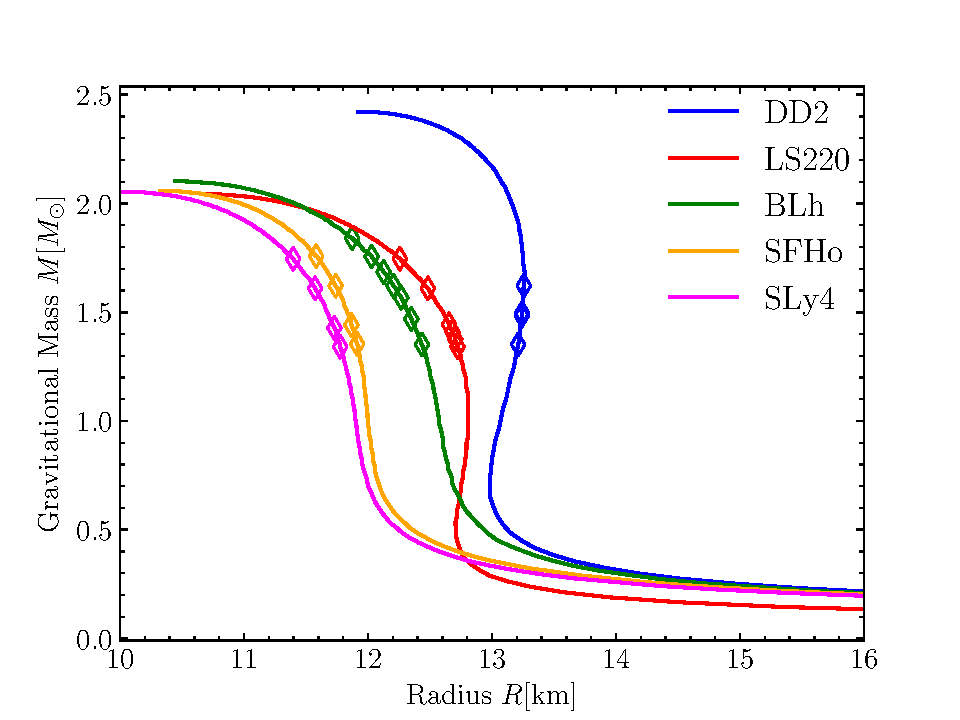
\includegraphics[width=0.49\textwidth]{tov_mr.pdf}
    \caption{Mass-radius relations for the EOSs used in this work. 
        Markers along the sequences indicate the NSs smulated in this work.}  
    \label{fig:method:tov_mr}
\end{figure}

For our models we employ $5$ finite-temperature, composition-dependent equations of state, namely the 
HS(DD2) (hereafter DD2) \cite{Typel:2009sy,Hempel:2009mc}, 
BLh, \cite{Bombaci:2018ksa}, 
LS220, \cite{Lattimer:1991nc}, 
HS(SFHo), (hereafter SFHo) \cite{Steiner:2012rk} and 
SLy4-SOR EOS (hereafter SLy4) \cite{daSilvaSchneider:2017jpg}.

All EOS include neutrinos $(n)$, protons $(p)$, nuclei, electrons, positrons, and photons
as important thermodynamic degrees of freedom.

The radii and maximum masses of neutron stars composed of the cold, neutrino-less $\beta$-equilibrium matter,
from these EOS, fall in line with the current astrophysical constraints, 
\textit{e.g.,} LIGO/Virgo constrain on tidal deformability 
\citep{TheLIGOScientific:2017qsa,Abbott:2018wiz,De:2018uhw,Abbott:2018exr}

All EOS models have symmetry energy at saturation density that are in argeement with experimental limits.
Notably, the LS220 has a especially steep dependency of its symmetry energy on density (\textit{e.g.,} \cite{Lattimer:2012xj,Danielewicz:2013upa}. Thus, this EOS might predict too low symmetry energy below the saturation density. 

%% LS220
The LS220 EOS is based on a non-relativistic (liquid droplet) Skyrme model.
The absolute value of the nuclear bulk incompressibility is set to $220$~MeV, hence, the name.
The EOS includes surface effects and it models $\alpha$-particles as an ideal, classical
non-relativistic gas. For heavy nuclei, the single nucleus approximation is sued. 
%Thus, the the compressible, liquid-drop model with surface effects and composed of ideal gas of 
%particles and heavy nuclei is used to represent the non-homogeneous nuclear matter.
%Heavy nuclei are considered with single nucleus approximation. 
The Gibbs construction is used to model the transition between homogeneous and non-homogeneous matter.
LS220 does not satisfy the constraints from Chiral effective field theory \cite{Hempel:2017ikt}

%% DD2
DD2 (and SFHo) employs the statistical equilibrium to treat the ensemble of several thousands nuclei.
The high-density nuclear matter is treated via RMF approach for unbound nucleons \cite{Hempel:2009mc}.
The excluded volume mechanism is utilized for the phase transition from nuclei to homogeneous
nuclear matter (when densities approch the nuclear saturation density).
DD2 employs the linear, but density dependent coupling for modeling the mean-field nuclear interactions \cite{Typel:2009sy}.
It was however noted that DD2 is not in very good agreement with the so-called flow-constraint \cite{Danielewicz:2002pu}.

%% SFHo [more rephrasing needed!]
Similar to DD2, SFHo combines a statistical ensemble of numerous nuclei, under the assumption of nuclear
statistical equilibrium (NSE) to treat the homogeneous matter, 
with the relativistic mean field approach for the unbound nucleons to treat high-density homogeneous nuclear matter.
It however employs a different parameterizations and values for modeling the mean-field nuclear interactions, 
which is motivated by neutron star radius measurements from low-mass X-ray
binaries (\cite{Steiner:2012rk} and references therein).

The DD2 and SFHo are based on nuclear statistical equilibrium, but 
different parameterizations of the covariant Lagrangian which models the mean-field nuclear interactions.
In these EOSs a finite volume correction coupled to a relativistic mean field theory for treating high-density nuclear matte. However, between these EOSs mean-field nuclear interactions have different parameterizations and values.

%% SLy4
The SLy4 EOS eomplyed in this work is the finite temperature extension \cite{daSilvaSchneider:2017jpg}
of the basic SLY4 Skryme parametrisation for cold nuclear NS matter \cite{Douchin:2001sv}.
The extension includes the non-local isospin asymmetric terms as well as more sophisticated 
treatment of nuclear surface properties and consistent treatment of heavy nuclei size. 
Which is a more advanced version of LS220 treatment (model).
When the phase transition, between the uniform and non-uniform phases, occurs, the phase with lowest 
free energy is chosen, (first order transition).

%% BLh
BLh is a new finite temperature EOS \cite{Logoteta:2020yxf}
This EOS is a finite temperature extension of the cold, $\beta$-equilibrium EOS, \cite{Bombaci:2018ksa},
which was applied to model the BNS merger in \cite{Endrizzi:2018uwl}.
The equation of state is derived in the framework of non-relativistic Brueckner-Hartree-Fock approach.
where microphysical approach based on a specific nuclear interaction is employed for the homogeneous nuclear phase.
The interactions between nucleos are described through a potential derived perturbatively 
in Chiral-Effective-Field theory \cite{Machleidt:2011zz}
The two body interactions are modeled up to second (from the leading term) order, that are used to calculate the local potential. This potential includes $\Delta$-resonances possible excitation. 
Further, the potential is augmented with the three-nucleon force, with the addition of $\Delta$-excitations.
The three-nucleon force was calibrated to reproduce the symmetric nuclear matter at saturatuin density \cite{Logoteta:2016nzc}.
The non-homogeneous phase of the EOS is treated by smoothly connecting the high density BLh EOS to the low-density oart of the SFHo EOS.


\subsubsection{Finite temperature treatment}


Thermal effects are included a different way in these EOS. 
In particular particle correlations beyond the mean field approximation are included only in the BLh EOS.
In other EOS thermal effects enter in the nucleon effective mass, that depend on temperature and density.
These effects, however, are important for the thermal evolution of the NS matter.

%% LS220 and SLy4
In the EOSs that are based on the Skyrme effecrive nuclear interatcions, \textit{e.g.,} LS220 and SLy4
the thermal effects are added in the following form. 
Consider a zero temperature internal energy functional, which depends explicitly on the nuclear density.
The part of this functional that is resposible for interactions is divided into the 
subpart that represents the two-body nucleon-nucleon interactions, (it is quadratic in nuclear density) and a 
subpart that mimics the effect of many body nuclear forces (proportional to the nuclear density in certain power).
Then, both the single particle potentials as well as kinetic energy effective mass dependence play a role
in the temperature dependence of the nuclear effective interaction.
The single particle potential are computed via the variation of the internal energy with respect to the 
neutron and proton densities.
Thus, the smaller the effective masss the larger are kinetic energies and hence, hgiher matter temperature. 
If the entropy remains unchainched.
Thus, the finite temperature behavior of these EOSs is largely set by the nucleon effective mass.
%Then, the smaller the effective mass, the higher the temperature (assuming that entropy is unchanged).
For LS220, the nucleon mass is its bare nucleon mass (for any densities) \gray{so... $m_{N}^*=m_{N}$??}.
For SFHo, $m_N ^* / m_N = 0.76$ at saturation density. 
For DD2 $m_N^*/m_N = 0.56$ 
For BLh $\red{None}$ 
For SLy4 $m_N^*/m_N=0.70$ at saturation density. 
where $m_{N}^*$ is the effective nucleon mass and $m_N$ is the bare nucleon mass.

%% SFHo (and DD2??)
For the SFHo and DD2 EOS, the relativistic Lagrangian considers the $\sigma-$, $\omega-$ and $\rho-$
meson exchanges for descibing nuclear interactions, and the mean-field approximation is used
to solve the resulted Euler-Largrange equations. 
The thermal effects for various species are introduced via Fermi-Dirac distributions at finite temperatures.
Then, self consitent solution of the mean filed eqution introduces the temperature dependence into other 
thermodynamic quantities (through fiurst mesons and nucleon fields)

%% BLh
The BLh EOS employs a different approach to incorporate temperature effects.
The method is based on evaluating the free energy in the Brueckner-Hartree-Fock, which in turn requires,
the effective in-medium nuclear interactions to be defined (starting from the bare nuclear potential).
\gray{This effective interaction is obtained by solving
    the Bethe-Goldstone integral equation which describe the nucleon 
    scattering in the nuclear medium and properly takes into
    account the Pauli principle}.
Then, the nucleon single particle potentials are evaluated (via integration of the on-shell effective interaction matrix)
, which represent the mean field that a nucleon with a certain momenum experience surrounded by other nucleons.
The nucleon single particle potentials, then, allow to evaulate the free energy, and subsequently, 
other thermodynamic quantities.
Notable difference with other EOS discussed here is that the many-body correlations extend beyond the mean field approximation, and are not present in other EOS. 
This EOS was first employed for the BNS merger simulations in \cite{Bernuzzi:2020txg}.

\subsubsection{TOV}

To characterize these EOS, that employs very different microphyscis and finite temperature properties and their relation to the electron fraction, we consider the TOV solutions, presented on the figure \ref{fig:method:tov_mr}.
The maximum mass of a non-rotating NS that these EOSs support are $2.06$, $2.06$, $2.42$ $None$ $None$ 
for SFHo, LS220, DD2, BLh and SLy4 respectively. The NS radii, $R_{1.4}$, then $11.9$, $12.7$, $13.2$ $\red{None}$ $\red{None}$, which in turn is related to the pressure at half saturation density \cite{Lattimer:2012nd}. Thus we adopt the following naming convention for EOS. Those that lead to a NS with smaller radii are called "softer" and those that lead to a NS with larger radii are referred to as "stiffer" EOS.
Among considered, the DD2 is the stiffest EOS, while SLy4 is the softest.

%% =====================================================================================
%%
%%               C O D E -- W H I S K Y - T H C
%%
%% =====================================================================================


\section{Code}


\subsection{Initial Data}

For Each EOS considered, we compute the irrotational BNS configurations in quasi-circular orbit.
We employ the pseudo-spectral code \texttt{Lorene} \citep{Gourgoulhon:2000nn}, that 
solves the general relativistic initial data problem.
The initial separation (of the qusi-circular orbit) is chosen $\sim40$~km and that corresponds to $~2-3$ orbits before merger.

The EOS table used for the initial data computation is the minimum temperature slice
$(T\sim 0.5 - 0.1)$~MeV of the finite temperature EOS table used for the evolution.
The assumption of the neutrino-less beta-equilibrium is made.
At constant temperature, at lowest densities, the photon energy (radiation) is a dominant contribution to 
pressure. Thus, we substruct this contribution from the tables.
%Addiitionally, the assuming constant temperature, we also remove the photon (radiation) energy contribution to the pressure (which dominates at the lowest densities)

The EOS table for the minimum temperature slice of the EOS table used for the evolution assuming neutrino-less beta-equilibrium.
Assuming constant temperature, we also remove the photon energy contribution to the pressure.

%In the evolution code, passing the initial data, the mapping is done from the zero temerature
In the evolution code, the electron fraction is set by the beta equilibrium condition. 
The specific internal energy is reset in accordance with minimum temperature slice of the EOS table used for evolution.

Errors present in the initial data in introduced during the mapping result in a small oscillations of netron stars.
In terms of relative changes in central density these amounts to $\sim2-3\%$ \cite{Radice:2018pdn}


\subsection{Evolution with \texttt{WhiskyTHC}}


In this part we review the numerical relativity code that was used to model binary neutron star mergers analyzed in this thesis.
The part is based on the David Radice PhD thesis where most of the methods are discussed \cite{Radice:2013apa}, and on the published results and regarding code structure and \cite{Radice:2012cu,Radice:2013xpa,Radice:2013hxh,Radice:2015nva}.

In order to perform numerical simulations of fluid flow, accurate numerical codes are essencial. Codes that flux-conservative finite-difference HRSC schemes offer a ciertain degree of simplicity, while high-order finite volume schemes are more computationally expensive (as they require solution of multiple Riemann problems at the interface between regions) \cite{Reisswig:2009us,Shu:2001rep} as well as complex averaging and de-averaging procedures \cite{Tchekhovskoy:2007zn}.

The \texttt{THC} code is the Templated-Hydrodynamics Code developed using the \texttt{Cactus} framework \cite{Goodale:2003}. In \texttt{THC}, the state-of-the-art flux-vector splitting scheme are employed. The "templated" in the code name stands for a modern paradigm in C++ programming, the templated programming, where a part of the code can be generated from the prescribed templates at compiling time (\textit{e.g.,} \cite{Yang:2001})

The \texttt{THC} has several primitive cariable reconstruction schemes implemented, such as MP5, classical monotonicity preserving \cite{Suresh:1997,Mignone:2010} the weighted essentially non oscillatory (WENO) schemes WENO5 and WENO7 \cite{Liu:1994,Jiang:1996,Shu:1997} and two bandwidth-optimized WENO schemes WENO3B and WENO4B \cite{Martin:2006,Taylor:2007}, contracted for modeling the compressible turbulence. Note, that the number in scheme name stands for a formal order of accuracy.

\texttt{WhiskyTHC} is a result of combination of two \texttt{Whisky} \cite{Baiotti:2004wn} and \texttt{THC} \cite{Radice:2012cu}. High-order flux-vector splitting finite-differencing techniques came from the former, while the module for the recovery of the primitive quantities as well as the equation of state framework from the latter \cite{Galeazzi:2013mia}. Tabulated temperature and composition dependent equation of states can be used.

Overall, \texttt{WhiskyTHC} solves the equations of general-relativistic hydrodynamics in conservation form \ref{eq:theory:grhdeq_thc} using a finite difference scheme. \red{tripple check the FD is used for space time evol and central FV method is for hydro}
The flux reconstruction is done in local-characteristic variables using the MP5 scheme, see \textit{e.g.,} \cite{Rezzolla:2013} \red{CHECK}.
The space-time is evolved using the CCZ4 formulation \ref{eq:theory:ccz4equations}, solved via finite difference code publicly available through \texttt{Einstein Toolkit}, \cite{McLachlan,Loffler:2011ay}.\red{CHECK}.
There, the central stencil is used throughout, and only terms associated with the advection along the shift vector are treated using the upwinded by one grid point stencil. The accuracy of the scheme is available at 6th and 8th order, while 4th is commonly employed. In addition, the fifth order Kreiss-Oliger style artificial dissipation \cite{Kreiss:1973} is added to aid with non-linear stability.

The code is build on the \texttt{Carpet} AMR driver \cite{Schnetter:2003rb} from the \texttt{Cactus} computational toolkit \cite{Goodale:2003}, incorporating a provided by \texttt{Carpet} Berger-Oliger-style mesh refinement \cite{Berger:1989,Berger:1984} with subcycling in time and refluxing. \textcolor{red}{in Thesis it is said, -- no refluxing was done yet}

To treat the vacuum region, the code utilizes common, 'atmosphere' approach. The atmosphere is referred to an artificial density floor in the simulation domain. It is introduced in order to tackle the challenges arising when considering boundary between the fluid and vacuum in Eulerian (relativistic) hydrodynamics codes \cite{Galeazzi:mThesis:2008,Kastaun:2006,Millmore:2009dk}. 
The defining property of the atmosphere is that the rest mass density and coordinate velocity are reset to a floor values once the former falls below a certain threshold value during the evolution \cite{Font:2001ew,Baiotti:2004wn}. While showing a reasonable results in second order codes, in higher order ones the numerical oscillations lead to the creation of vacuum nonetheless, that in light of the aforemention atmosphere effect result in the mass and energy violation \cite{Radice:2011qr}. For codes that rely on characteristic variables, the degeneracy in low-density, low-temperature limits also plagues the computation. This problem is the main reason behind the popularity of robust shock capturing codes, even though they are of first order in the general-relativistic hydrodynamics codes. Vacuum treatment for higher order codes is of main challenges to overcome.

There are several approaches in how to treat atmosphere. 

\textit{Standard atmosphere Treatment} or \textit{"ordinary MP5 approach"} is based on setting density that falls below $(1+\epsilon)\rho_{\text{atmo}}$ to the atmosphere density, velocity to zero and internal energy to the one prescubed by the polytropic EoS. The $\rho_{\text{atmo}}$ is usually related to a certain characteristic density, \textit{e.g.,} maximum density at the beginning of the simulation as $\rho_{\text{atmo}} = 10^{-7,-9}\rho_{\text{max}}$. The tolerance parameter $\epsilon$ is usually set to $10^{-2}$ and accounts for excessive oscillations of the fluid–vacuum interface. 

\textit{An Improved Atmosphere Treatment} or \textit{"MP5+LF"} In this approach the component-wise Lax-Friedrichs flux split is turned on when a certain density is reached. This increases the dissipation of the scheme and allows to avoid problems arising in characteristic reconstruction, associated with the degeneracy of the characteristic variables close to vacuum. Unfortunately, if the ejection of low velocity and density matter is concerned, this approach may yield oscillatory solutions and thus creates artifacts. 

\textit{Positivity Preserving Limiter} is an approach discussed in \cite{Radice:2013apa} based on the use of PPL proposed in \cite{Hu:2013}. \gray{Here we provide a brief overview}. \red{No, we not}.
\gray{While for a simplified case of classical gas dynamics it might require a lower timestep, in the general relativistic case and general tabulated EOS, the positivist of pressure is difficult to assure due to complexity of the energy source terms. It can be mitigated by enforcing a floor value on the pressure}. 
Note, that adopting a positivity preserving limiter to treat the transition between matter and vacuum, still implies replacing the vacuum with low density fluid at rest, is not a physically accurate approach. That would rely on treating the transition as a free boundary (see \textit{e.g.,} \cite{Kastaun:2006}) The advantage of positivity preserving limiter with respect to a classical atmosphere treatment, is that it allows to have a value of $\rho_{\text{atmo}}$ that does not require further tuning and can be arbitrary small, and assure that the solution is locally conserved. 
\textcolor{red}{In our models} we employ this approach as follows, at the beginning of the simulations we set the floor density, relying in the subsequent evolution on a positivity preserving limiters to ensure the atmosphere well behavior. Due to negligible density of the atmosphere its accretion has a negligible effect on the evolved object. 

For the extensive tests of different reconstruction methods and atmosphere treatment we refer to the \cite{Radice:2013apa}.


\subsection{Hydrodynamics}



\red{THE IDEA IS THAT YOU PUT MAIN EQ AND THEORY INTO THEORY AND HERE JUST USE THE 'PAPER' STUFF}

The code evolves the proton and neutron number densities, $n_n$ and $n_p$
respectively, as 

\begin{equation}
\label{eq:wthc:pndens}
\nabla_\nu (n_p u^\mu) = R_p^\mu \ \ , \ \ 
\nabla_\nu (n_n u^\mu) = R_n^\mu \ .
\end{equation}

\gray{in Radice2016dwd it is $\nabla_{\alpha}(n_e u^{\alpha}) = R$}

\gray{in Galezzi2013, for Whisky, the equations are separate for baryon and leptons: $\nabla_{\alpha}(n_bu^{\alpha})=0$ and $\nabla_{\alpha}(n_eu^{\alpha})=N$, where the $n_b$ and $n_e$ are the baryon and electron number densities respectively.}

Here $u^{\mu}$ is the fluid four-velocity, $R_p = -R_n$ is the net
lepton number deposition rate due to the absorption and emission of neutrinos 
and antineutrinos (\red{see Section XXX})

The $R_{p,n}$ is computed according to the neutrino M0 scheme \cite{Radice:2016dwd,Radice:2018pdn}

The number densities are related as $n_p=Y_e n$ where $n = n_p + n_e$ is the baryon 
number density and $Y_e$ is electron fraction.

The matter of a neutron star is approximated with ideal fluid with stress-energy tensor

\begin{equation}
T_{\mu\nu} = \rho h u_{\mu} u_{\nu} + Pg_{\mu\nu}
\end{equation}

where $\rho=m_{\text{b}} n$ is the baryon rest-mass density, 
$n$ the baryon number density, $m_{\text{b}} \simeq 10^{-24}\,$g 
the neutron mass, 
\gray{if Galezzi13 it is nucleon mass which is actrually related to the EOS.}
$h=1+\epsilon + P/\rho$ the specific enthalpy, 
$\epsilon$ the specific internal energy (energy density),
and $P$ is \gray{total isotropic} pressure.

Written in a covariant form, the Euler equation for balance of energy and momentum reads

\begin{equation}
\label{eq:wthc:euler}
\nabla_\nu T^{\mu\nu} = Q u^{\mu} \ ,
\end{equation}

\gray{in Radice2016dwd it is $\nabla_{\beta}T^{\alpha\beta}=\Psi^{\alpha}$
    with $\Psi^{\alpha} = Q u^{\alpha}$.
}
\gray{In the Galezzi:2013 it is $\nabla_{\alpha}T^{\alpha\beta}=\Psi^{\beta}$.
    There the $T^{\alpha\beta}$ accounts for the ordinary matter and for trappend neutrinos and photons, but it does not include free-streaming neutrinos. Assumed to be similar to the 'test-fluid' they are neglected in constracting RHS of the Eistein equations.
}

where $Q$ is the net energy deposition rate doe to absorption
and emission of neutrinos also treated with the M0 scheme.
\red{JUST PUT REFS TO THE EQs THAT ARE IN THE 'nuetrino' AND 'viscosity' sections}


\subsection{Numerical methods}


High resolution shock capturing methods are used to discritize equations 
\eqref{eq:wthc:euler} and \eqref{eq:wthc:pndens}.
Specifically, central Kurganov-Tadmor type scheme \cite{Kurganov:2000} with 
HLLE flux formula \cite{Einfeldt:1988}
and non-oscillatory reconstruction of the primitive variables with the MP5 scheme of
\cite{Suresh:1997}.

Shock capturing schemes require the presence of a low density atmosphere around neutron stars.
The constant value of $\rho_0 = m_p n \approx 6\times 10^4$~\gcm.

The rest-mass consirvation in the presence of artificial atmosphere is assured via 
positivity-preserving limiter from \cite{Radice:2013xpa}

The local number densities of neutrons and protons separately, are assured via 
multi-fluid advection method of \cite{Plewa:1998nma}

The outflow properties are extracted when the density exceeds the atmosphere density
by several orders of magnitude.

%% Spacetime evolution
The spacetime is evolved using the Z4c formulation of Einstein's equations
\cite{Bernuzzi:2009ex,Hilditch:2012fp} as implemented in the \texttt{CTGamma} code
\cite{Pollney:2009yz,Reisswig:2013sqa} which is part of the \texttt{Einstein Toolkit} 
\cite{Loffler:2011ay}.

The non-linear stability of evolution is assured via Kreiss-Oliger dissipation. 
The spacial discritisation is done via fourth-order finite-differencing implemented in \texttt{CTGamma}.

The method of lines, MOL, couples the space-time evolution and hydrodynamics. 

Time integrator of choice is strongly-stability preserving third-order Runge-Kutta scheme \cite{Gottlieb:2009}.
The timestep is regulated by the Courant-Friedrichs-Lewy (CFL) condition, that required CFL factor 
to be $<0.25$ for numerical stability. To assure taht the positivity-preserving limiter implemented in \texttt{WhiskyTHC} maintains the density positive, the CFL factor is set to $0.15$.


\subsection{AMR}


The code uses the Berger-Oliger conservative adaptive mesh renement (AMR) \cite{Berger:1984} with 
sub-cycling in time and \red{refluxing (Davids thesis does not have refluxing)} \cite{Berger:1989,Reisswig:2012nc} as provided by the \texttt{Carpet module} of the \texttt{Einstein Toolkit} 
\cite{Schnetter:2003rb}. 


\subsection{Neutrino scheme}


\begin{table}
    \caption{
        Weak reactions employed in our simulations and references for their implementation.
        In the left column, $\nu \in \{\nu_e, \bar{\nu}_e, \nu_{x}\}$ denotes any neutrino species, 
        $\nu_{x}$ any heavy-lepton neutrinos, $N \in\{n, p\}$ a nucleon, and $A$ any nucleus.
        In the central column the role of each reaction is highlighted, with "P" standing for 
        production, "A" for absorption opacity and "S" for scattering opacity. When two roles are
        indicated, the second refers to the inverse ($\leftarrow$) reaction.
        Table is taken from \cite{Radice:2018pdn}.
    }
    \label{tab:leakage}
    \begin{center}
        \begin{tabular}{lll}
            \hline\hline
            Reaction & Role &  Ref. \\ 
            \hline
            $p + e^- \leftrightarrow \nu_e + n $          & P,A & \cite{Bruenn:1985}  \\
            $n + e^+ \leftrightarrow \bar{\nu}_{e} + p $  & P,A & \cite{Bruenn:1985}  \\
            $e^+ + e^- \rightarrow \nu + \bar{\nu}$       & P & \cite{Ruffert:1995fs} \\
            $\gamma + \gamma \rightarrow \nu + \bar{\nu}$ & P & \cite{Ruffert:1995fs} \\
            $N + N \rightarrow \nu + \bar{\nu} + N  + N$  & P & \cite{Burrows:2004vq} \\
            $\nu + N \rightarrow \nu + N$                 & S & \cite{Ruffert:1995fs} \\
            $\nu + A \rightarrow \nu + A$                 & S & \cite{Shapiro:1983du} \\
            \hline\hline
        \end{tabular}
    \end{center}
\end{table}

\red{JUST Name the chemes and reference the equations}
\red{JUST PUT REFS TO THE EQs THAT ARE IN THE 'nuetrino' AND 'viscosity' sections}

\subsection{Code General Setup}



The simulation domain is a cube of $3.024$~km each side, whose center is at the center of mass pf the binary.
The AMR structure has $7$ refinemnt levels, with the finest convering both compact objects during the inspiral and the remnant postmerger.

We consider several resolution setups. Low resolution (LR) simulations have $h=246$~m, standard resolution (SR) 
have $h=185$~m and high resolution (HR) $h=123$~m for the final refinemnt level.

In the simulations where the neutirno M0 scheme is included, it is switched on shortly before the merger. 
The equations \eqref{eq:method:whisky:eq7} and \eqref{eq:method:whisky:eq9} are solved on the uniform spherical grid
with radius $\approx 756$~km, and resolution $n_r\times n_{\theta}\times n_{\phi} = 3096 \times 32 \times 64$
grid points.

A subset of models discussed in this thesis include the effective treatment of viscosity. 

We consider \red{$33$} distinct binary with total masses $\red{[None,None]}$ and mass-ratio $q\in[1.00,1.82]$.
In all models the neutrino leackage plus M0 scheme. Most models were computed at at least two resolutions. 
Most our models also include the effect of subgrid turbulence, viscosity.

\gray{Summary of all results in given in the table...}

\gray{Each run is nameed as}

\gray{We simulate each model for at least $\red{None}$~ms after the merger or a few milliseconds after BH formation}


%% =====================================================================================
%%
%%               P O S T - P R O C E S S I N G
%%
%% =====================================================================================


\section{Postprocessing tools and methods}


In order to investigate the neutron star merger dynamics and outflowing material we imploy the following methods and tools.

In order to study and compara on a quantiative level properties of outflow, disk and remnant we employ the mass-averaged quantities and for a quantity $f$ they are computed as 
\begin{equation}
\langle f \rangle = \frac{\sum_i f(m_i)m_i}{\sum_i m_i}
\end{equation}
where $m_i$ is the mass contained in the $i$-th bin.


\subsection{Disk \& Remnant}

It is common to discuss the post-merger state of the binary neutron star systems in terms of the remnant, a neutron star or a black hole, and a disk or torus. However there is not unified convention in how to define the latter and separate it from the former. 

In the case where the remnant is a BH, the disk common disk definition is the matter outside the apparent horizon, (\eg, \cite{Dietrich:2015iva,Dietrich:2016hky}). 
However, owing to the disk accretion onto a black hole, the extraction time is a crutual paramter, and unfortunately is not consistent in the literature, (\eg $\sim1$~ms in \cite{Dietrich:2015iva,Dietrich:2016hky} and $\sim30$~ms in \cite{Sekiguchi:2016bjd}).

In the case where the remnant is a neutron star, the disk definition usually includes the density cut. For instance, in \cite{Radice:2018pdn,Kiuchi:2019lls,Vincent:2019kor} the disk is assumed to encompass the matter with $\rho < 10^{13}$~\gcm. 
The threshold $\rho\sim 10^{13}$~\gcm corresponds to the point in the remnant where
the angular velocity profiles becomes approximately Keplerian, \citep[\eg][]{Shibata:2005ss,Shibata:2006nm,Hanauske:2016gia,Kastaun:2016elu}.
The extraction time here is also important, but less so, as we find that the accretion on the NS is considerably slower.

Overall, we estimate that these differences can amount to a systematic factor of a few,
which we employ for the statistical analysis in section \ref{sec:stat:anal}

% In this thesis we define the disk as a matter that satisfies two criteria $\alpha > 0.15$ and $\tho < 10^{13}\gcm$, where $\alpha$ is the lapse function (see section \ref{sec:theory:gr3p1}).

We compute the baryonic mass of the disks is computed as the volume integral of the conserved rest-mass density $D=\sqrt{\gamma}~W\rho$,

\begin{equation}
\label{eq:method:mdisk}
M_{\text{disk}} = \int D \dd^3 x
\end{equation}

from 3D snapshots of the simulations in postprocessing.



%% In \cite{Sekiguchi:2016bjd}, the disk mass is extracted at
%% ${\approx} 30$~ms outside the AH. In \cite{Radice:2018pdn}, the disk mass is computed
%% as the baryonic mass outside the AH at BH formation, while for NS
%% remnants the criterion $\rho < 10^{13}$ g cm$^{-3}$ is used. 
%% In \cite{Kiuchi:2019lls} for both BH and NS outcome the $\rho < 10^{13}$ g cm$^{-3}$ 
%% criterion is used and time of the extraction is not specified. 
%% In \cite{Vincent:2019kor} the density criterion is the same, however the simulations 
%% are significantly shorter (${~\sim 7.5}$~ms) than in other
%% works. Overall, we estimate that these differences can amount to a
%% systematic factor of a few.



\subsection{Density modes}

%% FROM THE LETTER 

The hydrodynamic instability is monitored by a decomposition in Fourier modes
$e^{-\i m\phi}$ of the Eulerian rest-mass density on the equatorial plane 
[see Eq.~(1) of \citep{Radice:2016gym}] and characterized by the
development of a $m=2$ followed by a $m=1$ mode 
\citep{East:2015vix,Paschalidis:2015mla,Radice:2016gym,Lehner:2016wjg,Bernuzzi:2013rza,Kastaun:2014fna}.
In the short-lived remnant (LS220) the $m=1$ mode
is subdominant with respect to the $m=2$, and it reaches a maximum close to the collapse
\citep{Bernuzzi:2013rza}. Instead, in the long-lived remnant (DD2) the $m=1$
becomes the dominant mode at $\sim$20~ms and persists throughout the
remnant's lifetime, while the $m=2$ efficiently dissipates via
gravitational-wave emission \citep{Bernuzzi:2015opx,Radice:2016gym}.

%% FROM THE PAPER 

During the post-merger evolution the neutron star oscillates. The most prominant modes are quasiradial mode $F$ ($m=0$), the $m=2$ $f$-model and non-linear combinations of them \citep[\eg][]{Shibata:2000jt,Stergioulas:2011gd}.

It has also been shown that the $m=1$, one-armed spiral instability, is present in the remnant of neutron star mergers \citep{Paschalidis:2015mla,Radice:2016gym,East:2016zvv}.

In order to investigate the dynamical instabilities in our simulations we 
project the rest-mass density onto spherical harmonics,
or, in other words, we perform the complex azimuthal mode decomposition of,
the conserved rest-mass density.
For simplicity we consider only $\rho(x,y,z=0,t)$, 
\ie restrict our analysis to the orbital plane $z=0$

\red{DOUBLE check the presence of Gamma and W}
%% \begin{equation}
%% \label{eq:modes}
%% C_m = \int \rho(x,y,z=0,t) W e^{-i m \phi} \sqrt{\gamma} %% \text{d}x \text{d} y \, ,
%% \end{equation}
\begin{equation}
\label{eq:modes}
C_m(t) = \int \rho(x,y,z=0,t) e^{-i m \phi(x,y)} \text{d}x \text{d} y \, ,
\end{equation}
(see \eg~\citet{Baiotti:2009gk}).

% where %% $\rho$ is the rest mass density, 
% $\gamma$ is the determinant of the three-metric and $W$ is the
% Lorentz factor between the fluid and the Eulerian observers. 

Note that the above quantities are gauge dependent.

\red{Dietrich in his thesis thinks that the growing m=1 mode is "We can not
    exclude the possibility that the growing m = 1 mode is triggered by numerical effects,
    but we think that it is a physical hydrodynamical effect due to mode couplings."
    Page 53 of the thesis
}

In addition, friequencies of the modes can be computed with the Fourier analysis of the $\rho_{\text{max}}$ and projections $C_{m}$. We resort it for the future work, as in this work we are interested inly in their magnitude. 





\subsection{Angular momentum}

\red{First, white that in GR the angular momentum is not clearly defined}

%% FROM LETTER 

From the fluid's stress energy tensor,
we compute the angular momentum density flux $J_r = T_{ra}(\partial_\phi)^a$,
where $\phi$ is the cylindrical angular coordinate;
angular momentum is conserved if $(\partial_\phi)^a$ is a Killing vector.

%% FROM PAPER 

The fluid's angular momentum analysis in the remnant and disk is performed
assuming axisymmetry (see Appendix~\ref{app:ang} for derivation).
That is, we assume $\phi^{\mu} = (\partial_{\phi})^{\mu}$ to be a Killing
vector. Accordingly, the conservation law
\begin{equation}
\partial_t(T^{\mu\nu}\phi_{\nu}n_{\nu}\sqrt{\gamma}) -
\partial_i(\alpha T^{i \nu}\phi_{\nu}\sqrt{\gamma}) = 0 \ ,
\end{equation}
where $n^\mu$ is the normal vector to the spacelike hypersurfaces of
the spacetime's $3+1$ decomposition, 
implies the conservation of the angular momentum
\begin{equation}
J = % \int j dV = 
%- \int \, T_{\mu\nu}n^{\mu}\phi^{\nu}\,\dd ^3x = 
-\int \,
T_{\mu\nu}n^{\mu}\phi^{\nu}\,\sqrt{\gamma}\, \dd^3 x\ .
\end{equation}
In the cylindrical coordinates $x^i=(r,\phi,z)$ adapted to the symmetry
the angular momentum density is  
\begin{equation}
j = %-
\rho h W^2 v_{\phi} \ ,
\label{eq:method:ang_mom}
\end{equation}
and the angular momentum flux is 
\begin{equation}
\alpha\sqrt{\gamma}T^r _{\nu}\phi^{\nu} =
\alpha\sqrt{\gamma}\rho h W^2 (v^{r}v_{\phi}) .
\end{equation}


\subsection{Ejecta}


To model and study the electromagnetic counterparts to mergers, the amount and properties of the material
leaving the system are needed.
The matter expelled at high velocity may ultimately become unbound from the central gravitational
potential. There are two indicators commonly adopted to mark the unbound matter.

\subsubsection{The Geodesic criterion}

Assuming that the spacetime is stationary, the $\partial_t$ is the killing vectory \red{confirm}, 
the four-velocity, $u_t$, (along the time-like killing vector), is a constant of motion for geodesics. 
Additionally, if the space is asymptotically flat, at infinity the $u_t = -W$, where $W$ is the fluid element Lorentz factor. Then, if a fluid element has $u_t < -1$, it may be considered unbound \red{as it will retain the non-zero positive velocity at infinity}. 
The fluid reaches an asymptotic velocity 
\begin{equation}
\upsilon_{\infty} \simeq \sqrt{2E_{\infty}} = \sqrt{(1-u_t ^2)}.
\end{equation}
The criterion can be through of as considering the fluid to be made of isolated particles that follow the geodesics. Indeed, the effects of equation of state, fluids pressure gradient, internal energy and heating (\eg, due to an $r$-process (\red{see section XXX})) are neglected. The space time is also assumed to be static.
Strictly speaking, none of these assumptions is fulfilled in the BNS post-merger environment. However, this criterion is widely used in the literature \citep[\eg][]{Radice:2018pdn,Vincent:2019kor}.
Note that the geodesic criterion above neglects the fluid's pressure and might underestimate the ejecta mass.

\subsubsection{The Bernoulli criterion}

From the relativistic Bernoulli equation \citep{Rezzolla:2013}, it follows
that for a stationary relativisitc flow, the $hu_t$ is constnat along the 
fluid worldliens. Here $h$ is the (relativistic) enthalpy, which is
defined up to a constant factor. 
If at the spatial infinity the enthalpy is set so $h\rightarrow-1$, 
\red{in Vincent it is $h\leftarrow 1$}
the condition $hu_t < -1$ would mark the unbound matter 
(as in the assymptotically flat space-time the $u_t = -W$ for the flow particles following geodesics).

The associated asymptotic velocity is calculated as 
\begin{equation}
\upsilon_{\infty} \simeq \sqrt{2 (h (E_{\infty}+1)-1)}. 
\end{equation}

The criterion can be regarded as assuming all the internal energy of the fluid 
gets added to the fluid kinetic energy, as the fluid decompresses \red{(pressure drops?)}.

The $r$-process nucleosynthesis that occurs in the outflow deposits the energy.
\red{In Vincent it is assumed that the difference in binding energy between the 
    particles in NSE at a given $\rho$, $T$ and $Y_e$, and their binding energy at
    the same $Y_e$ but low $\rho$ and $T$ is added/substracted from the fluid's kinetic energy.
    Out-of-NSE evolution and effects this neglected \citep[][see]{Foucart:2016vxd}
    [BUT I AM NOT SURE IF THIS IS THE CASE FOR OUR SIMULATIONS! MAYBE NOT!]}

This criterion has been found to estimate more accurately the amount of unbound material \citep{Foucart:2015gaa}
However, as was also found that the Bernoulli criterion leads to up to twice the amount of ejecta detected in comparion with the geodensic criterion, if the estimation is done within a given volume \citep{Kastaun:2014fna}.

We adopt the geodesic criterion to study the "burst-like", short outflows,
such as dynamical ejecta, where the pressure gradient is not expected to make a significant contribution.
For the steady-state outflows, like postmerger winds we adopt the Bernoulli criterion.

The term ejecta would refer to the material gravitationaly unbound according to eather of the criteria.




All considered mass ejecta are calculated on a coordinate sphere at $R \simeq 294$km. 
\red{untill afterglow}




%% =====================================================================================
%%
%%               R E S U L T S
%%
%% =====================================================================================


\section{Results}


\red{
    To be defined: \\
    Chirp pass \\
    Gravitational and Baryonic masses
}

In this chapter we review the findings of \citet{Nedora:2019jhl} and \citet{Nedora:2020pak}
and investigate the long-term \pmerg{} evolution of the binary neutron star. 

Such studies are of high astrophysical importance as the ejecta of matter that occur 
on various timescales \pmerg{} undergoes \rproc{} and produces observable EM emission. 
The discussion of the \rproc{} and EM transits themselves, we resort for the chapter \red{chap:coutnerparts}.


\subsection{Simulations}




%% --------------------------------
%% TAB SIM SUMMARY
%\begin{table*}
\begin{sidewaystable}
\begin{center}
\captionsetup{width=1.0\linewidth}
    \caption{
      Summary table of all the simulations and dynamical ejecta properties. The columns contain
      the following information, starting from the left. Equation of
      state, mass-ratio, available resolutions,
      inclusion of subgrid turbulence, time of the
      simulation end, time of the BH formation for LR, SR, HR
      resolutions separately, time of last output, time the disk mass
      is extracted, disk mass, mass of the
      dynamical ejecta, mass-averaged electron fracton, terminal
      velocity and RMS angle (from the binary plane) for dynamical ejecta. For all
      data except $t_{BH}$, $t_{\text{end}}$ and $t_{\text{disk}}$, the value that is given is a mean value across resolutions, with an error estimated as one
      standard diviaion from the mean. In case where only one
      resolution is present, the error is assumed to be $20\%$ of the
      value. Adopted from \citet{Nedora:2020pak}.
    }
      %% \newtxt{For discussions on errors and convergence see \citep{Radice:2018pdn,Bernuzzi:2020txg}.
      %% The model data are available online at \citep{vsevolod_nedora_2020_4159619}.
%%       }
\scalebox{0.70}{
\begin{tabular}{c c c c c c c c c c c c c}
    \hline\hline
    EOS & $q$ & $\tilde{\Lambda}$ & Resolution & GRLES & $t_{\text{end}}$ & $t_{\text{BH}}$ & $t_{\text{disk}}$ & $M_{\text{disk}} ^{\text{last}}$ & $\md$ & $\langle \yd \rangle$ & $\langle \vd  \rangle$ & $\langle \theta_{\text{ej}} ^{\text{d}} \rangle$ \\
    &   &   &  &  & [ms] & [ms] & [ms] &   & $[10^{-2} M_{\odot}]$ &   & $[c]$ &   \\ 
    \hline
    \hline
    BLh & 1.00 & 541 & \texttt{LR SR HR} & \cmark & $43.3$ $91.8$ $23.1$ & $>43.3$ $>91.8$ $>23.1$ & 23.1 & $0.166^{+0.052} _{-0.052} $ & $0.14^{+0.02} _{-0.02} $ & $0.27^{+0.01} _{-0.01} $ & $0.17^{+0.01} _{-0.01} $ & $39.65^{+0.35} _{-0.35} $ \\
    BLh & 1.00 & 541 & \texttt{LR SR} & \xmark & $15.9$ $103.2$ $ $ & $>15.9$ $>103.2$ $ $ & 15.6 & $0.261^{+0.008} _{-0.008} $ & $0.12^{+0.01} _{-0.01} $ & $0.27^{+0.01} _{-0.01} $ & $0.16^{+0.01} _{-0.01} $ & $38.80^{+0.44} _{-0.44} $ \\
%%  BLh & 1.00 & 541 & \texttt{LR SR} & \xmark & $36.9$ $15.5$ $ $ & $>36.9$ $>15.5$ $ $ & 36.6 & $0.182^{+0.091} _{-0.091} $ & $0.21^{+0.04} _{-0.04} $ & $0.26^{+0.01} _{-0.01} $ & $0.18^{+0.01} _{-0.01} $ & $36.29^{+0.24} _{-0.24} $ \\
    \hline
    BLh & 1.18 & 539 & \texttt{LR} & \cmark & $69.4$ $ $ $ $ & $>69.4$ $ $ $ $ & 69.0 & $0.202^{+0.101} _{-0.101} $ & $0.30^{+0.06} _{-0.06} $ & $0.18^{+0.04} _{-0.04} $ & $0.19^{+0.04} _{-0.04} $ & $33.65^{+6.73} _{-6.73} $ \\
    BLh & 1.18 & 539 & \texttt{LR} & \xmark & $16.4$ $ $ $ $ & $>16.4$ $ $ $ $ & 15.9 & $0.229^{+0.115} _{-0.115} $ & $0.25^{+0.05} _{-0.05} $ & $0.16^{+0.03} _{-0.03} $ & $0.20^{+0.04} _{-0.04} $ & $30.86^{+6.17} _{-6.17} $ \\
    \hline
    BLh & 1.34 & 539 & \texttt{LR SR} & \cmark & $63.4$ $9.8$ $ $ & $>63.4$ $>9.8$ $ $ & 9.8 & $0.192^{+0.004} _{-0.004} $ & $0.25^{+0.05} _{-0.05} $ & $0.14^{+0.04} _{-0.04} $ & $0.17^{+0.00} _{-0.00} $ & $28.79^{+5.00} _{-5.00} $ \\
    BLh & 1.34 & 539 & \texttt{LR} & \xmark & $18.0$ $ $ $ $ & $>18.0$ $ $ $ $ & 18.0 & $0.211^{+0.106} _{-0.106} $ & $0.19^{+0.04} _{-0.04} $ & $0.17^{+0.03} _{-0.03} $ & $0.17^{+0.03} _{-0.03} $ & $33.39^{+6.68} _{-6.68} $ \\
    \hline
    BLh & 1.43 & 540 & \texttt{LR SR} & \cmark & $35.1$ $59.6$ $ $ & $>35.1$ $>59.6$ $ $ & 33.8 & $0.265^{+0.001} _{-0.001} $ & $0.27^{+0.08} _{-0.08} $ & $0.19^{+0.03} _{-0.03} $ & $0.16^{+0.00} _{-0.00} $ & $34.49^{+3.59} _{-3.59} $ \\
    \hline
    BLh & 1.54 & 543 & \texttt{LR} & \cmark & $45.8$ $ $ $ $ & $>45.8$ $ $ $ $ & 53.8 & $0.324^{+0.162} _{-0.162} $ & $0.20^{+0.04} _{-0.04} $ & $0.17^{+0.03} _{-0.03} $ & $0.13^{+0.03} _{-0.03} $ & $31.21^{+6.24} _{-6.24} $ \\
    BLh & 1.54 & 543 & \texttt{LR} & \xmark & $17.4$ $ $ $ $ & $>17.4$ $ $ $ $ & 30.1 & $0.287^{+0.144} _{-0.144} $ & $0.22^{+0.04} _{-0.04} $ & $0.21^{+0.04} _{-0.04} $ & $0.16^{+0.03} _{-0.03} $ & $35.05^{+7.01} _{-7.01} $ \\
    \hline
    BLh & 1.66 & 538 & \texttt{LR SR} & \cmark & $64.6$ $20.1$ $ $ & $>64.6$ $1.8$ $ $ & 19.2 & $0.289^{+0.005} _{-0.005} $ & $0.42^{+0.05} _{-0.05} $ & $0.11^{+0.01} _{-0.01} $ & $0.12^{+0.01} _{-0.01} $ & $24.08^{+0.29} _{-0.29} $ \\
    \hline
    BLh & 1.82 & 532 & \texttt{LR SR HR} & \cmark & $12.0$ $17.5$ $9.6$ & $1.4$ $1.4$ $1.5$ & 5.9 & $0.170^{+0.001} _{-0.001} $ & $0.81^{+0.04} _{-0.04} $ & $0.03^{+0.01} _{-0.01} $ & $0.11^{+0.00} _{-0.00} $ & $6.53^{+0.65} _{-0.65} $ \\
    BLh & 1.82 & 532 & \texttt{LR SR HR} & \xmark & $53.8$ $26.3$ $45.2$ & $1.7$ $1.3$ $1.0$ & 43.2 & $0.098^{+0.049} _{-0.049} $ & $1.07^{+0.07} _{-0.07} $ & $0.03^{+0.01} _{-0.01} $ & $0.12^{+0.00} _{-0.00} $ & $6.27^{+0.53} _{-0.53} $ \\
    \hline
    \hline
    DD2 & 1.00 & 853 & \texttt{LR SR}    & \xmark & $92.0$ $110.2$       & $>92.0$ $>110.2$        & 9.4 & $0.154^{+0.052} _{-0.052} $ & $0.11^{+0.01} _{-0.01} $ & $0.25^{+0.00} _{-0.00} $ & $0.18^{+0.01} _{-0.01} $ & $38.07^{+0.52} _{-0.52} $ \\
    DD2 & 1.00 & 853 & \texttt{LR SR HR} & \cmark & $123.0$ $113.0$ $74.4$ & $>123.0$ $>113.0$ $>74.4$ & 8.2 & $0.111^{+0.040} _{-0.040} $ & $0.12^{+0.03} _{-0.03} $ & $0.27^{+0.01} _{-0.01} $ & $0.16^{+0.00} _{-0.00} $ & $40.03^{+0.71} _{-0.71} $ \\
    \hline
    DD2 & 1.20 & 847 & \texttt{LR SR HR} & \xmark & $37.3$ $91.0$ $55.2$ & $>37.3$ $>91.0$ $>55.2$ & 36.6 & $0.261^{+0.028} _{-0.028} $ & $0.21^{+0.08} _{-0.08} $ & $0.18^{+0.03} _{-0.03} $ & $0.17^{+0.01} _{-0.01} $ & $29.07^{+3.75} _{-3.75} $ \\
    DD2 & 1.22 & 847 & \texttt{LR SR HR} & \cmark & $42.7$ $107.3$ $19.8$ & $>42.7$ $>107.3$ $>19.8$ & 8.7 & $0.209^{+0.033} _{-0.033} $ & $0.25^{+0.02} _{-0.02} $ & $0.19^{+0.01} _{-0.01} $ & $0.17^{+0.01} _{-0.01} $ & $30.74^{+0.89} _{-0.89} $ \\
    \hline
    DD2 & 1.43 & 820 & \texttt{LR SR} & \cmark & $37.7$ $62.0$ $ $ & $>37.7$ $>62.0$ $ $ & 36.7 & $0.304^{+0.051} _{-0.051} $ & $0.70^{+0.64} _{-0.64} $ & $0.14^{+0.05} _{-0.05} $ & $0.14^{+0.01} _{-0.01} $ & $25.51^{+9.58} _{-9.58} $ \\
    \hline
    \hline
    LS220 & 1.00 & 715 & \texttt{LR SR} & \cmark & $27.0$ $27.1$ $ $ & $13.7$ $13.7$ $ $ & 16.1 & $0.073^{+0.032} _{-0.032} $ & $0.16^{+0.02} _{-0.02} $ & $0.25^{+0.02} _{-0.02} $ & $0.16^{+0.01} _{-0.01} $ & $35.70^{+0.78} _{-0.78} $ \\
    LS220 & 1.00 & 715 & \texttt{LR SR HR} & \xmark & $35.9$ $37.2$ $27.1$ & $33.4$ $16.1$ $15.4$ & 34.6 & $0.072^{+0.006} _{-0.006} $ & $0.16^{+0.06} _{-0.06} $ & $0.22^{+0.00} _{-0.00} $ & $0.16^{+0.01} _{-0.01} $ & $34.99^{+1.68} _{-1.68} $ \\
    \hline
    LS220 & 1.05 & 715 & \texttt{SR HR} & \xmark & $ $ $23.3$ $24.1$ & $ $ $17.3$ $13.9$ & 22.3 & $0.107^{+0.054} _{-0.054} $ & $0.16^{+0.02} _{-0.02} $ & $0.21^{+0.01} _{-0.01} $ & $0.16^{+0.01} _{-0.01} $ & $33.28^{+2.37} _{-2.37} $ \\
    LS220 & 1.11 & 717 & \texttt{SR HR} & \xmark & $ $ $25.1$ $24.4$ & $ $ $17.0$ $>24.4$ & 24.2 & $0.140^{+0.071} _{-0.071} $ & $0.22^{+0.03} _{-0.03} $ & $0.19^{+0.02} _{-0.02} $ & $0.18^{+0.02} _{-0.02} $ & $30.25^{+4.43} _{-4.43} $ \\
    \hline
    LS220 & 1.16 & 714 & \texttt{SR HR} & \cmark & $ $ $95.8$ $11.3$ & $ $ $68.9$ $>11.3$ & 95.5 & $0.306^{+0.153} _{-0.153} $ & $0.34^{+0.00} _{-0.00} $ & $0.22^{+0.00} _{-0.00} $ & $0.16^{+0.00} _{-0.00} $ & $34.08^{+1.00} _{-1.00} $ \\
    LS220 & 1.16 & 714 & \texttt{LR SR HR} & \xmark & $29.5$ $36.1$ $28.8$ & $>29.5$ $>36.1$ $24.1$ & - & - & $0.33^{+0.05} _{-0.05} $ & $0.17^{+0.01} _{-0.01} $ & $0.17^{+0.01} _{-0.01} $ & $30.01^{+0.64} _{-0.64} $ \\
    \hline
    LS220 & 1.43 & 710 & \texttt{LR SR} & \cmark & $19.8$ $28.5$ $ $ & $15.7$ $12.3$ $ $ & 19.6 & $0.178^{+0.072} _{-0.072} $ & $0.73^{+0.03} _{-0.03} $ & $0.16^{+0.02} _{-0.02} $ & $0.17^{+0.01} _{-0.01} $ & $26.77^{+3.50} _{-3.50} $ \\
    \hline
    LS220 & 1.66 & 707 & \texttt{LR SR} & \cmark & $6.8$ $8.0$ $ $ & $1.4$ $2.1$ $ $ & 2.0 & $0.068^{+0.008} _{-0.008} $ & $1.11^{+0.38} _{-0.38} $ & $0.07^{+0.01} _{-0.01} $ & $0.14^{+0.01} _{-0.01} $ & $13.18^{+1.33} _{-1.33} $ \\
    \hline
    \hline
    SFHo & 1.00 & 413 & \texttt{SR HR} & \cmark & $ $ $25.3$ $11.6$ & $ $ $6.0$ $4.0$ & 50.0 & $0.023^{+0.012} _{-0.012} $ & $0.40^{+0.07} _{-0.07} $ & $0.21^{+0.00} _{-0.00} $ & $0.19^{+0.01} _{-0.01} $ & $32.48^{+1.79} _{-1.79} $ \\
    SFHo & 1.00 & 413 & \texttt{LR SR HR} & \xmark & $3.2$ $7.7$ $9.0$ & $>3.2$ $4.1$ $3.8$ & 7.2 & $0.019^{+0.007} _{-0.007} $ & $0.28^{+0.07} _{-0.07} $ & $0.23^{+0.01} _{-0.01} $ & $0.21^{+0.01} _{-0.01} $ & $31.66^{+1.80} _{-1.80} $ \\
    \hline
    SFHo & 1.13 & 412 & \texttt{SR HR} & \cmark & $ $ $14.2$ $14.3$ & $ $ $6.3$ $>14.3$ & - & - & $0.44^{+0.12} _{-0.12} $ & $0.18^{+0.01} _{-0.01} $ & $0.23^{+0.01} _{-0.01} $ & $33.20^{+0.78} _{-0.78} $ \\
    SFHo & 1.13 & 412 & \texttt{LR SR HR} & \xmark & $16.5$ $19.3$ $15.2$ & $5.5$ $11.6$ $3.9$ & 15.1 & $0.046^{+0.041} _{-0.041} $ & $0.42^{+0.03} _{-0.03} $ & $0.17^{+0.03} _{-0.03} $ & $0.22^{+0.01} _{-0.01} $ & $29.63^{+4.39} _{-4.39} $ \\
    \hline
    SFHo & 1.43 & 414 & \texttt{LR} & \cmark & $19.6$ $ $ $ $ & $4.8$ $ $ $ $ & 18.9 & $0.201^{+0.101} _{-0.101} $ & $0.38^{+0.08} _{-0.08} $ & $0.14^{+0.03} _{-0.03} $ & $0.20^{+0.04} _{-0.04} $ & $29.20^{+5.84} _{-5.84} $ \\
    SFHo & 1.43 & 414 & \texttt{SR} & \cmark & $ $ $46.5$ $ $ & $ $ $>46.5$ $ $ & 50.8 & $0.241^{+0.121} _{-0.121} $ & $0.24^{+0.05} _{-0.05} $ & $0.19^{+0.04} _{-0.04} $ & $0.14^{+0.03} _{-0.03} $ & $32.86^{+6.57} _{-6.57} $ \\
    \hline
    SFHo & 1.66 & 408 & \texttt{LR SR} & \cmark & $11.2$ $16.8$ $ $ & $1.3$ $1.3$ $ $ & 11.6 & $0.177^{+0.153} _{-0.153} $ & $0.15^{+0.00} _{-0.00} $ & $0.07^{+0.00} _{-0.00} $ & $0.12^{+0.01} _{-0.01} $ & $10.39^{+1.14} _{-1.14} $ \\
    \hline
    \hline
    SLy4 & 1.00 & 402 & \texttt{LR SR} & \cmark & $10.5$ $13.1$ $ $ & $2.8$ $2.8$ $ $ & - & - & $0.09^{+0.02} _{-0.02} $ & $0.23^{+0.02} _{-0.02} $ & $0.27^{+0.02} _{-0.02} $ & $30.81^{+2.81} _{-2.81} $ \\
    SLy4 & 1.00 & 402 & \texttt{LR SR} & \xmark & $12.7$ $22.0$ $ $ & $2.7$ $13.8$ $ $ & 12.5 & $0.071^{+0.175} _{-0.175} $ & $0.31^{+0.20} _{-0.20} $ & $0.23^{+0.03} _{-0.03} $ & $0.22^{+0.01} _{-0.01} $ & $32.23^{+4.84} _{-4.84} $ \\
    \hline
    SLy4 & 1.13 & 402 & \texttt{LR SR} & \xmark & $8.4$ $20.3$ $ $ & $>8.4$ $13.0$ $ $ & 8.0 & $0.164^{+0.023} _{-0.023} $ & $0.59^{+0.07} _{-0.07} $ & $0.16^{+0.00} _{-0.00} $ & $0.24^{+0.01} _{-0.01} $ & $29.67^{+1.97} _{-1.97} $ \\
    \hline
    SLy4 & 1.43 & 399 & \texttt{SR} & \cmark & $ $ $40.3$ $ $ & $ $ $>40.3$ $ $ & 45.2 & $0.200^{+0.100} _{-0.100} $ & $0.20^{+0.04} _{-0.04} $ & $0.21^{+0.04} _{-0.04} $ & $0.15^{+0.03} _{-0.03} $ & $34.03^{+6.81} _{-6.81} $ \\
    \hline
    SLy4 & 1.66 & 397 & \texttt{SR} & \cmark & $ $ $7.2$ $ $ & $ $ $1.2$ $ $ & 3.9 & $0.138^{+0.069} _{-0.069} $ & $0.28^{+0.06} _{-0.06} $ & $0.05^{+0.01} _{-0.01} $ & $0.12^{+0.02} _{-0.02} $ & $8.43^{+1.69} _{-1.69} $ \\
    \hline\hline
\end{tabular}
\label{tab:sim}
}%scalebox
\end{center}
%\end{table*}
\end{sidewaystable}



%\usepackage{lipsum}% dummy text
%\begin{document}
    %\lipsum % Text before
%    \afterpage{%
%        \clearpage% Flush earlier floats (otherwise order might not be correct)
%        \thispagestyle{empty}% empty page style (?)
%        \begin{landscape}% Landscape page
%            \centering % Center table
%            \begin{tabular}{c c c c c c c c c c c c c}
%                \hline\hline
%                EOS & $q$ & $\tilde{\Lambda}$ & Resolution & GRLES & $t_{\text{end}}$ & $t_{\text{BH}}$ & $t_{\text{disk}}$ & $M_{\text{disk}} ^{\text{last}}$ & $\md$ & $\langle \yd \rangle$ & $\langle \vd  \rangle$ & $\langle \theta_{\text{ej}} ^{\text{d}} \rangle$ \\
%                &   &   &  &  & [ms] & [ms] & [ms] &   & $[10^{-2} M_{\odot}]$ &   & $[c]$ &   \\ 
%                \hline
%                \hline
%                BLh & 1.00 & 541 & \texttt{LR SR HR} & \cmark & $43.3$ $91.8$ $23.1$ & $>43.3$ $>91.8$ $>23.1$ & 23.1 & $0.166^{+0.052} _{-0.052} $ & $0.14^{+0.02} _{-0.02} $ & $0.27^{+0.01} _{-0.01} $ & $0.17^{+0.01} _{-0.01} $ & $39.65^{+0.35} _{-0.35} $ \\
%                BLh & 1.00 & 541 & \texttt{LR SR} & \xmark & $15.9$ $103.2$ $ $ & $>15.9$ $>103.2$ $ $ & 15.6 & $0.261^{+0.008} _{-0.008} $ & $0.12^{+0.01} _{-0.01} $ & $0.27^{+0.01} _{-0.01} $ & $0.16^{+0.01} _{-0.01} $ & $38.80^{+0.44} _{-0.44} $ \\
%                %%  BLh & 1.00 & 541 & \texttt{LR SR} & \xmark & $36.9$ $15.5$ $ $ & $>36.9$ $>15.5$ $ $ & 36.6 & $0.182^{+0.091} _{-0.091} $ & $0.21^{+0.04} _{-0.04} $ & $0.26^{+0.01} _{-0.01} $ & $0.18^{+0.01} _{-0.01} $ & $36.29^{+0.24} _{-0.24} $ \\
%                \hline
%                BLh & 1.18 & 539 & \texttt{LR} & \cmark & $69.4$ $ $ $ $ & $>69.4$ $ $ $ $ & 69.0 & $0.202^{+0.101} _{-0.101} $ & $0.30^{+0.06} _{-0.06} $ & $0.18^{+0.04} _{-0.04} $ & $0.19^{+0.04} _{-0.04} $ & $33.65^{+6.73} _{-6.73} $ \\
%                BLh & 1.18 & 539 & \texttt{LR} & \xmark & $16.4$ $ $ $ $ & $>16.4$ $ $ $ $ & 15.9 & $0.229^{+0.115} _{-0.115} $ & $0.25^{+0.05} _{-0.05} $ & $0.16^{+0.03} _{-0.03} $ & $0.20^{+0.04} _{-0.04} $ & $30.86^{+6.17} _{-6.17} $ \\
%                \hline
%                BLh & 1.34 & 539 & \texttt{LR SR} & \cmark & $63.4$ $9.8$ $ $ & $>63.4$ $>9.8$ $ $ & 9.8 & $0.192^{+0.004} _{-0.004} $ & $0.25^{+0.05} _{-0.05} $ & $0.14^{+0.04} _{-0.04} $ & $0.17^{+0.00} _{-0.00} $ & $28.79^{+5.00} _{-5.00} $ \\
%                BLh & 1.34 & 539 & \texttt{LR} & \xmark & $18.0$ $ $ $ $ & $>18.0$ $ $ $ $ & 18.0 & $0.211^{+0.106} _{-0.106} $ & $0.19^{+0.04} _{-0.04} $ & $0.17^{+0.03} _{-0.03} $ & $0.17^{+0.03} _{-0.03} $ & $33.39^{+6.68} _{-6.68} $ \\
%                \hline
%                BLh & 1.43 & 540 & \texttt{LR SR} & \cmark & $35.1$ $59.6$ $ $ & $>35.1$ $>59.6$ $ $ & 33.8 & $0.265^{+0.001} _{-0.001} $ & $0.27^{+0.08} _{-0.08} $ & $0.19^{+0.03} _{-0.03} $ & $0.16^{+0.00} _{-0.00} $ & $34.49^{+3.59} _{-3.59} $ \\
%                \hline
%                BLh & 1.54 & 543 & \texttt{LR} & \cmark & $45.8$ $ $ $ $ & $>45.8$ $ $ $ $ & 53.8 & $0.324^{+0.162} _{-0.162} $ & $0.20^{+0.04} _{-0.04} $ & $0.17^{+0.03} _{-0.03} $ & $0.13^{+0.03} _{-0.03} $ & $31.21^{+6.24} _{-6.24} $ \\
%                BLh & 1.54 & 543 & \texttt{LR} & \xmark & $17.4$ $ $ $ $ & $>17.4$ $ $ $ $ & 30.1 & $0.287^{+0.144} _{-0.144} $ & $0.22^{+0.04} _{-0.04} $ & $0.21^{+0.04} _{-0.04} $ & $0.16^{+0.03} _{-0.03} $ & $35.05^{+7.01} _{-7.01} $ \\
%                \hline
%                BLh & 1.66 & 538 & \texttt{LR SR} & \cmark & $64.6$ $20.1$ $ $ & $>64.6$ $1.8$ $ $ & 19.2 & $0.289^{+0.005} _{-0.005} $ & $0.42^{+0.05} _{-0.05} $ & $0.11^{+0.01} _{-0.01} $ & $0.12^{+0.01} _{-0.01} $ & $24.08^{+0.29} _{-0.29} $ \\
%                \hline
%                BLh & 1.82 & 532 & \texttt{LR SR HR} & \cmark & $12.0$ $17.5$ $9.6$ & $1.4$ $1.4$ $1.5$ & 5.9 & $0.170^{+0.001} _{-0.001} $ & $0.81^{+0.04} _{-0.04} $ & $0.03^{+0.01} _{-0.01} $ & $0.11^{+0.00} _{-0.00} $ & $6.53^{+0.65} _{-0.65} $ \\
%                BLh & 1.82 & 532 & \texttt{LR SR HR} & \xmark & $53.8$ $26.3$ $45.2$ & $1.7$ $1.3$ $1.0$ & 43.2 & $0.098^{+0.049} _{-0.049} $ & $1.07^{+0.07} _{-0.07} $ & $0.03^{+0.01} _{-0.01} $ & $0.12^{+0.00} _{-0.00} $ & $6.27^{+0.53} _{-0.53} $ \\
%                \hline
%                \hline
%                DD2 & 1.00 & 853 & \texttt{LR SR}    & \xmark & $92.0$ $110.2$       & $>92.0$ $>110.2$        & 9.4 & $0.154^{+0.052} _{-0.052} $ & $0.11^{+0.01} _{-0.01} $ & $0.25^{+0.00} _{-0.00} $ & $0.18^{+0.01} _{-0.01} $ & $38.07^{+0.52} _{-0.52} $ \\
%                DD2 & 1.00 & 853 & \texttt{LR SR HR} & \cmark & $123.0$ $113.0$ $74.4$ & $>123.0$ $>113.0$ $>74.4$ & 8.2 & $0.111^{+0.040} _{-0.040} $ & $0.12^{+0.03} _{-0.03} $ & $0.27^{+0.01} _{-0.01} $ & $0.16^{+0.00} _{-0.00} $ & $40.03^{+0.71} _{-0.71} $ \\
%                \hline
%                DD2 & 1.20 & 847 & \texttt{LR SR HR} & \xmark & $37.3$ $91.0$ $55.2$ & $>37.3$ $>91.0$ $>55.2$ & 36.6 & $0.261^{+0.028} _{-0.028} $ & $0.21^{+0.08} _{-0.08} $ & $0.18^{+0.03} _{-0.03} $ & $0.17^{+0.01} _{-0.01} $ & $29.07^{+3.75} _{-3.75} $ \\
%                DD2 & 1.22 & 847 & \texttt{LR SR HR} & \cmark & $42.7$ $107.3$ $19.8$ & $>42.7$ $>107.3$ $>19.8$ & 8.7 & $0.209^{+0.033} _{-0.033} $ & $0.25^{+0.02} _{-0.02} $ & $0.19^{+0.01} _{-0.01} $ & $0.17^{+0.01} _{-0.01} $ & $30.74^{+0.89} _{-0.89} $ \\
%                \hline
%                DD2 & 1.43 & 820 & \texttt{LR SR} & \cmark & $37.7$ $62.0$ $ $ & $>37.7$ $>62.0$ $ $ & 36.7 & $0.304^{+0.051} _{-0.051} $ & $0.70^{+0.64} _{-0.64} $ & $0.14^{+0.05} _{-0.05} $ & $0.14^{+0.01} _{-0.01} $ & $25.51^{+9.58} _{-9.58} $ \\
%                \hline
%                \hline
%                LS220 & 1.00 & 715 & \texttt{LR SR} & \cmark & $27.0$ $27.1$ $ $ & $13.7$ $13.7$ $ $ & 16.1 & $0.073^{+0.032} _{-0.032} $ & $0.16^{+0.02} _{-0.02} $ & $0.25^{+0.02} _{-0.02} $ & $0.16^{+0.01} _{-0.01} $ & $35.70^{+0.78} _{-0.78} $ \\
%                LS220 & 1.00 & 715 & \texttt{LR SR HR} & \xmark & $35.9$ $37.2$ $27.1$ & $33.4$ $16.1$ $15.4$ & 34.6 & $0.072^{+0.006} _{-0.006} $ & $0.16^{+0.06} _{-0.06} $ & $0.22^{+0.00} _{-0.00} $ & $0.16^{+0.01} _{-0.01} $ & $34.99^{+1.68} _{-1.68} $ \\
%                \hline
%                LS220 & 1.05 & 715 & \texttt{SR HR} & \xmark & $ $ $23.3$ $24.1$ & $ $ $17.3$ $13.9$ & 22.3 & $0.107^{+0.054} _{-0.054} $ & $0.16^{+0.02} _{-0.02} $ & $0.21^{+0.01} _{-0.01} $ & $0.16^{+0.01} _{-0.01} $ & $33.28^{+2.37} _{-2.37} $ \\
%                LS220 & 1.11 & 717 & \texttt{SR HR} & \xmark & $ $ $25.1$ $24.4$ & $ $ $17.0$ $>24.4$ & 24.2 & $0.140^{+0.071} _{-0.071} $ & $0.22^{+0.03} _{-0.03} $ & $0.19^{+0.02} _{-0.02} $ & $0.18^{+0.02} _{-0.02} $ & $30.25^{+4.43} _{-4.43} $ \\
%                \hline
%                LS220 & 1.16 & 714 & \texttt{SR HR} & \cmark & $ $ $95.8$ $11.3$ & $ $ $68.9$ $>11.3$ & 95.5 & $0.306^{+0.153} _{-0.153} $ & $0.34^{+0.00} _{-0.00} $ & $0.22^{+0.00} _{-0.00} $ & $0.16^{+0.00} _{-0.00} $ & $34.08^{+1.00} _{-1.00} $ \\
%                LS220 & 1.16 & 714 & \texttt{LR SR HR} & \xmark & $29.5$ $36.1$ $28.8$ & $>29.5$ $>36.1$ $24.1$ & - & - & $0.33^{+0.05} _{-0.05} $ & $0.17^{+0.01} _{-0.01} $ & $0.17^{+0.01} _{-0.01} $ & $30.01^{+0.64} _{-0.64} $ \\
%                \hline
%                LS220 & 1.43 & 710 & \texttt{LR SR} & \cmark & $19.8$ $28.5$ $ $ & $15.7$ $12.3$ $ $ & 19.6 & $0.178^{+0.072} _{-0.072} $ & $0.73^{+0.03} _{-0.03} $ & $0.16^{+0.02} _{-0.02} $ & $0.17^{+0.01} _{-0.01} $ & $26.77^{+3.50} _{-3.50} $ \\
%                \hline
%                LS220 & 1.66 & 707 & \texttt{LR SR} & \cmark & $6.8$ $8.0$ $ $ & $1.4$ $2.1$ $ $ & 2.0 & $0.068^{+0.008} _{-0.008} $ & $1.11^{+0.38} _{-0.38} $ & $0.07^{+0.01} _{-0.01} $ & $0.14^{+0.01} _{-0.01} $ & $13.18^{+1.33} _{-1.33} $ \\
%                \hline
%                \hline
%                SFHo & 1.00 & 413 & \texttt{SR HR} & \cmark & $ $ $25.3$ $11.6$ & $ $ $6.0$ $4.0$ & 50.0 & $0.023^{+0.012} _{-0.012} $ & $0.40^{+0.07} _{-0.07} $ & $0.21^{+0.00} _{-0.00} $ & $0.19^{+0.01} _{-0.01} $ & $32.48^{+1.79} _{-1.79} $ \\
%                SFHo & 1.00 & 413 & \texttt{LR SR HR} & \xmark & $3.2$ $7.7$ $9.0$ & $>3.2$ $4.1$ $3.8$ & 7.2 & $0.019^{+0.007} _{-0.007} $ & $0.28^{+0.07} _{-0.07} $ & $0.23^{+0.01} _{-0.01} $ & $0.21^{+0.01} _{-0.01} $ & $31.66^{+1.80} _{-1.80} $ \\
%                \hline
%                SFHo & 1.13 & 412 & \texttt{SR HR} & \cmark & $ $ $14.2$ $14.3$ & $ $ $6.3$ $>14.3$ & - & - & $0.44^{+0.12} _{-0.12} $ & $0.18^{+0.01} _{-0.01} $ & $0.23^{+0.01} _{-0.01} $ & $33.20^{+0.78} _{-0.78} $ \\
%                SFHo & 1.13 & 412 & \texttt{LR SR HR} & \xmark & $16.5$ $19.3$ $15.2$ & $5.5$ $11.6$ $3.9$ & 15.1 & $0.046^{+0.041} _{-0.041} $ & $0.42^{+0.03} _{-0.03} $ & $0.17^{+0.03} _{-0.03} $ & $0.22^{+0.01} _{-0.01} $ & $29.63^{+4.39} _{-4.39} $ \\
%                \hline
%                SFHo & 1.43 & 414 & \texttt{LR} & \cmark & $19.6$ $ $ $ $ & $4.8$ $ $ $ $ & 18.9 & $0.201^{+0.101} _{-0.101} $ & $0.38^{+0.08} _{-0.08} $ & $0.14^{+0.03} _{-0.03} $ & $0.20^{+0.04} _{-0.04} $ & $29.20^{+5.84} _{-5.84} $ \\
%                SFHo & 1.43 & 414 & \texttt{SR} & \cmark & $ $ $46.5$ $ $ & $ $ $>46.5$ $ $ & 50.8 & $0.241^{+0.121} _{-0.121} $ & $0.24^{+0.05} _{-0.05} $ & $0.19^{+0.04} _{-0.04} $ & $0.14^{+0.03} _{-0.03} $ & $32.86^{+6.57} _{-6.57} $ \\
%                \hline
%                SFHo & 1.66 & 408 & \texttt{LR SR} & \cmark & $11.2$ $16.8$ $ $ & $1.3$ $1.3$ $ $ & 11.6 & $0.177^{+0.153} _{-0.153} $ & $0.15^{+0.00} _{-0.00} $ & $0.07^{+0.00} _{-0.00} $ & $0.12^{+0.01} _{-0.01} $ & $10.39^{+1.14} _{-1.14} $ \\
%                \hline
%                \hline
%                SLy4 & 1.00 & 402 & \texttt{LR SR} & \cmark & $10.5$ $13.1$ $ $ & $2.8$ $2.8$ $ $ & - & - & $0.09^{+0.02} _{-0.02} $ & $0.23^{+0.02} _{-0.02} $ & $0.27^{+0.02} _{-0.02} $ & $30.81^{+2.81} _{-2.81} $ \\
%                SLy4 & 1.00 & 402 & \texttt{LR SR} & \xmark & $12.7$ $22.0$ $ $ & $2.7$ $13.8$ $ $ & 12.5 & $0.071^{+0.175} _{-0.175} $ & $0.31^{+0.20} _{-0.20} $ & $0.23^{+0.03} _{-0.03} $ & $0.22^{+0.01} _{-0.01} $ & $32.23^{+4.84} _{-4.84} $ \\
%                \hline
%                SLy4 & 1.13 & 402 & \texttt{LR SR} & \xmark & $8.4$ $20.3$ $ $ & $>8.4$ $13.0$ $ $ & 8.0 & $0.164^{+0.023} _{-0.023} $ & $0.59^{+0.07} _{-0.07} $ & $0.16^{+0.00} _{-0.00} $ & $0.24^{+0.01} _{-0.01} $ & $29.67^{+1.97} _{-1.97} $ \\
%                \hline
%                SLy4 & 1.43 & 399 & \texttt{SR} & \cmark & $ $ $40.3$ $ $ & $ $ $>40.3$ $ $ & 45.2 & $0.200^{+0.100} _{-0.100} $ & $0.20^{+0.04} _{-0.04} $ & $0.21^{+0.04} _{-0.04} $ & $0.15^{+0.03} _{-0.03} $ & $34.03^{+6.81} _{-6.81} $ \\
%                \hline
%                SLy4 & 1.66 & 397 & \texttt{SR} & \cmark & $ $ $7.2$ $ $ & $ $ $1.2$ $ $ & 3.9 & $0.138^{+0.069} _{-0.069} $ & $0.28^{+0.06} _{-0.06} $ & $0.05^{+0.01} _{-0.01} $ & $0.12^{+0.02} _{-0.02} $ & $8.43^{+1.69} _{-1.69} $ \\
%                \hline\hline
%            \end{tabular}
%            \captionof{table}{
%            Summary table of all the simulations and dynamical ejecta properties. The columns contain
%            the following information, starting from the left. Equation of
%            state, mass-ratio, available resolutions,
%            inclusion of subgrid turbulence, time of the
%            simulation end, time of the BH formation for LR, SR, HR
%            resolutions separately, time of last output, time the disk mass
%            is extracted, disk mass, mass of the
%            dynamical ejecta, mass-averaged electron fracton, terminal
%            velocity and RMS angle (from the binary plane) for dynamical ejecta. For all
%            data except $t_{BH}$, $t_{\text{end}}$ and $t_{\text{disk}}$, the value that is given is a mean value across resolutions, with an error estimated as one
%            standard diviaion from the mean. In case where only one
%            resolution is present, the error is assumed to be $20\%$ of the
%            value. Adopted from \citet{Nedora:2020pak}.
%        }% Add 'table' caption
%        \end{landscape}
%        \clearpage% Flush page
%    }
%    %\lipsum % Text after
%%\end{document}




























%% --------------------------------


In total we consider a sample of $37$ simulations of unique binaries with the 
chirp mass $\mathcal{M}_c = 1.188\,\Msun$ that corresponds to the source of \GW{}.
%% ---
The total gravitational mass covers the range $M\in[2.73, 2.88]\Msun$, while the 
mas ration $q=M_A/M_B\in[1,1.8]$. 
%% ---
We show the masses and radii of computed models as markers on the 
figure~\ref{fig:method:tov_mr} and summarize their main properties, 
and the dynamical ejecta properties in the table~\ref{tab:sim}.
%% --- 
Most simulations are performed with at least two resolutions, 
\texttt{LR} and \texttt{SR}. 
Additionally, $16$ binaries are simulataed at high resolution \texttt{HR}.
In total $76$ simulations are analyzed.
% ---
Several binaries that resulted in a formation of a MNS are evolved up to 
$100$~ms \pmerg.
%% ---
Most simulations include the effects of subgrid turbulence. 
Those that are not are marked with ``*'' next to the equation of state name.
%% --- 
The naming convention for simulations is the following: 
the equation of state name, the mass ratio, and the resolution, \eg, 
the ``BLh* $q=1.00$ (\texttt{SR})" would refer to the simulation of the equal mass
binary performed with BLh EOS, without subgrid turbulence and at standard resolution. 
%% ---
%% mass ratio binaries has been already presented in \cite{Bernuzzi:2020txg}.
%% Together with our previous data these simulations form the largest
%% sample of merger simulations with microphysics available to date
%% \citep{Bernuzzi:2015opx,Radice:2016dwd,Radice:2016rys,Radice:2017lry,Radice:2018xqa,Radice:2018pdn,Perego:2019adq,Endrizzi:2019trv,Bernuzzi:2020txg}.  


\subsection{Overview of the remnant dynamics}
\label{sec:bns_dynsmics_overview}


This section is based on the \cite{Nedora:2020pak}


\begin{figure}[t]
    \centering
    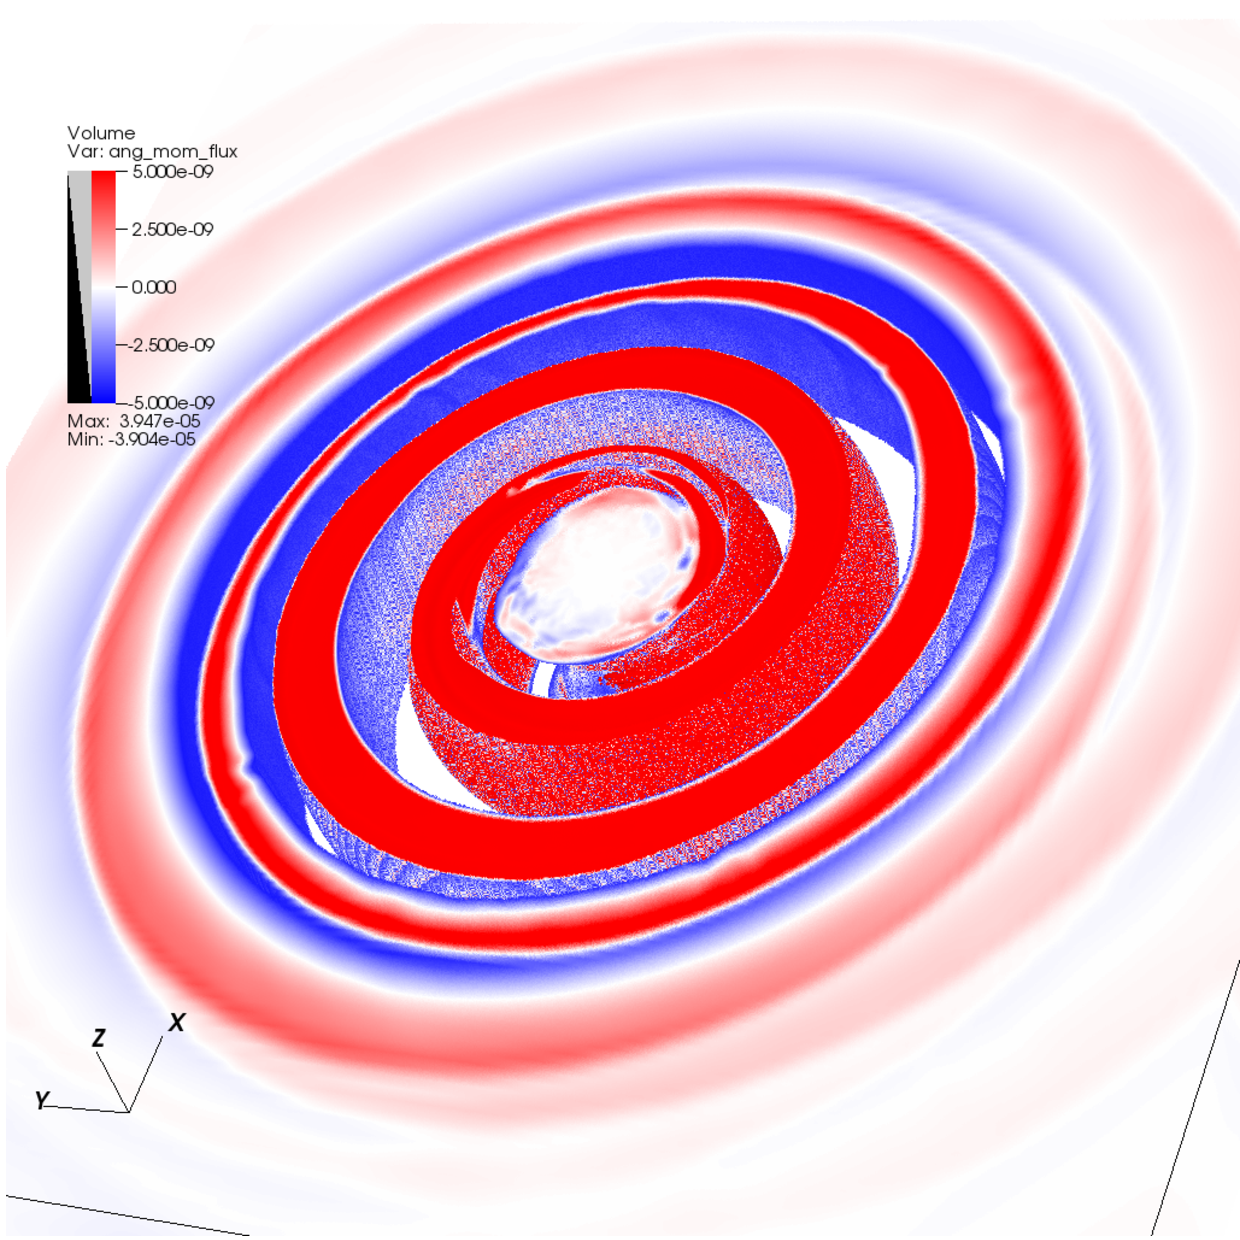
\includegraphics[width=0.49\textwidth]{raycasting_smooth_cropped.pdf}
    \caption{3D distribution of angular momentum density flux $J_r$
        from the DD2 simulation with turbulent viscosity at ${\sim}43.5$~ms after
        merger. $J_r$ is shown on a central region of
        $(89\times89\times60)$~km${}^3$ covering the remnant NS
        and disk, and it is given in units where $c=G=\Msun=1$.
        (Adapted from \citet{Nedora:2019jhl})
    }
    \label{fig:ang_mom_flux}
\end{figure}

\subsection{High mass ratio binaries}

Newly born \ac{MNS} is not axisymmetric. In addition to driving the angular 
momentum transport, it is a strong emittor of \acp{GW} at kiloHertz frequencies.
In ${\sim}10-20$~ms \pmerg{} the \acp{GW} remove about two time the 
amount of energy that was lost during the inspiral and merger \citep{Bernuzzi:2015opx}.
After that, the contribution of \acp{GW} to the system evolution, specifically to the angular momentum loss, drops \citep{Radice:2018xqa}. 
The long-term evolution, $\O(100)$~ms, of the remnant is driven primarely by the viscous processes and weak interactions.

After the emission of \acp{GW} subsides, the \acp{MNS} still have an excess in angular momentum and gravitational mass, with respect to the cold, rigidly rotating equilibrium with the same baryoinc mass \citep{Radice:2018xqa}.

The subsequent evolution of the \ac{MNS} is towards the axisymmetric configuration close to the mass-shedding limit. However, would a \ac{MNS} reach this state or collapse to a \ac{BH} depends on the details of \pmerg{} state and on the temperature and composition effects.


A subset of \ac{BNS} models with high mass-ratio forms a \ac{BH} 
during the merger \cite{Bernuzzi:2020txg}. The absence of the core bounce
is indicated by the monotonic increase of the central density.
Such a behavior is referred to as prompt collapse \citep{Radice:2020ddv,Bernuzzi:2020tgt,Bernuzzi:2020txg}.
Specifically, these are models with $q\gtrsim1.67$. 
\gray{During the merger, the companion star (less massive) undergoes a tidal disruption, as the tidal forces overcome the star's binding energy}. The star is then accreted onto the primary (most massive). 
The accretion raises its mass beyond the maximum supported limit by the \ac{EOS}, which leads to collapse. 
The newly formed \ac{BH} is surrounded by the accretion disk that was left from the tidally disrupted companion.

At formation, the disk has a large baryon mass, ${\sim}0.15\,\Msun$, in comparison with the disks formed in prompt collapse of equal mass binaries, \citep[\eg][]{Radice:2018pdn}. 
The disk is also neutron-rich $Y_e\sim 0.1$.

We show the evolution of the disk mass of several representative models in Fig.~\ref{fig:disk_mass_evo}.

\red{EJECTA to be moved to its own section}
The models that undergo the prompt collapse also eject matter on a dynamical timescale. The ejecta originates from tidal disruption of the compantion. It is neutron rich, confined largely to the orbital plane and exhibits a crescent-like azimuthal structure \citep{Bernuzzi:2020txg}.

\begin{figure}[t]
    \centering 
    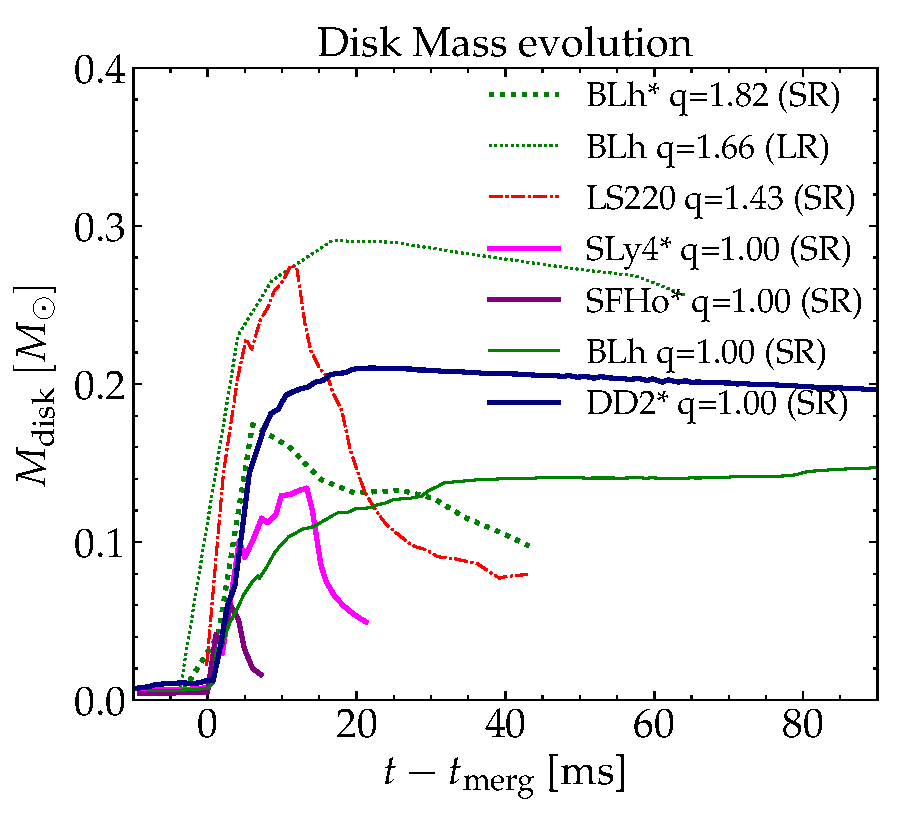
\includegraphics[width=0.49\textwidth]{disk/total_disk_mass_evo.pdf}
    \caption{Time evolution of the total disk mass for a few selected
        short-lived and long-lived cases. The former show a rapid 
        accretion right after disk formation. The plots show
        distinct difference in dynamical evolution after disk formation: accretion onto
        the newly formed BH (short-lived remnants) or accretion onto the NS
        remnant (DD2 $q=1$) with possible continuous mass shedding from the remnant
        into the disk (BLh* $q=1$). Adopted from \citet{Nedora:2020pak}
    } 
    \label{fig:disk_mass_evo}
\end{figure}


\subsubsection{Binaries with $q\lesssim1.4$}

Binaries with small mass ratio, ($q\lesssim1.4$) produce a \ac{MNS} remnant
that either survives on a dynamical timescale, set by the \ac{NS} rotation, before
collapsing to a \ac{BH}, or a \ac{MNS} that survives till the end of the simulations.
We refer to the former ones as \textit{short-lived} and the latter ones as 
\textit{long-lived} remnants.
Under the first category, fall the \ac{MNS} with relatively soft \ac{EOS}:
LS220 $q=1,1.1,1.2$, SFHo $q=1,1.1,1.4$ and SLy $q=1,1.1,1.4$. 
They collapse within $\sim20$~ms \pmerg. 
The exact time of the collapse however depends on the simulation resolution 
and on the inclusion of subgrid turbulence as was previosly noted by \citet{Radice:2017zta}.


\paragraph*{Disk of short-lived remnants}

During the merger, shocks generated at the collisional interface of the \acp{NS} cores,
as well as, tidal torques exerted by the non axisymmetric remnant result in a formation
of the disk. 
Matter, energy and angular momentum are injected into the disk as the spiral density waves 
propagate outwards from the mass-shedding \ac{MNS} remnant 
\citep{Bernuzzi:2015opx,Radice:2018xqa}.
\red{HERE the letter stuff could be added, actually}

%% --- Letter stuff
The spiral arms propagate from the remnant \ac{NS} into
the disk and transport angular momentum outwards as shown in
Fig.~\ref{fig:ang_mom_flux}. Such global density waves are a generic and
efficient mechanism to redistribute energy and eventually deplete  
accretion disks \citep{Goodman:2001a,Rafikov:2016a,Arzamasskiy:2018a}. 
%% Crucially, we find that both the $m=1$ and $m=2$ modes generate a \wind{} from the
%% disk's outer layers that is distinct from the dynamical ejecta, see Fig.~\ref{fig:ej_properties}.

Within these waves the fluid reaches highest temperatures, which decrease rapidly, as 
disk expansion and neutrino emission cools the matter. 
In such a high-temperature environment, the electron-positron pair creation is enhanced.
%% [added from Shibata Review paper]
As a result, neutrons can capture positrons $n+e^+p\rightarrow\bar{\nu}_e$.
The average particle energies are large, close to the mass difference between neutron 
and proton. 
In combination with the high $\nu_e$ and $\bar{\nu}_e$ luminosities,
the large number of available positrons leads to an increase 
in the fluid electron fraction, $Y_e$ from that of the initially neutron-rich material
\citep{Qian:1996xt}.
Additionally, a \ac{MNS} is a strong neutrino emitter. The neutrino irradiation of the 
surrounding area alters its composition, and neutrino absorption takes place
$n+\nu_e\rightarrow p + e^{-}$ and $p + \bar{\nu}_e\rightarrow n + e^+$.
This drives the neutron and proton fraction towards equilibrium, and raises the $Y_e$.
\red{paper says: 
    The electron fraction is reset by an initial excess of electron antineutrino emission
    and electron neutrino absorption,}
The entropy per baryon varies between $3$ and $\lesssim 10\,$$k_{B}$/baryon \citep{Perego:2019adq}.
%% ---
If \ac{MNS} remnant collapses to a BH, the main source of neutrinos shuts down and 
the inner part of the disk is rapidly accreted. 
The disk then approaches quasi-steady state, Fig.~\ref{fig:disk_mass_evo}, with 
axisymmetric, approximately Keplerian profile.
The inner part of the resulted disk, at densities $\rho\sim10^{13}$~\gcm, 
is relatively hot, $T\sim10\,$ MeV, but neutron-rich $Y_e\sim0.1$, as it was shielded 
from the neutrino irradiation. The disk gets progressively colder and proton-rich 
outwards with $Y_e$ reaching $0.4$ at the edges.
%% ---
The disk mass at formation appears to depend on the \ac{NS} \ac{EOS}. Binaries with 
stiffer EOS (larger \ac{NS} radii) produce more massive disk.
\red{[Fitting function]
    The disk mass can be described within the numerical uncertainties by a
    quadratic function of the mass ratio and the reduced tidal
    parameters (see Sec.~\ref{sec:remdisk}).}
Additionally, the disk mass show a dependency on mass ratio. For instance, the most massive disks are formed in LS220 $q=1.43$ and  BLh $q=1.82$ models, where the latter experiences prompt collapse.
%% -- 
The disk accretionon a \ac{BH} removes up to $50\%$ of the disk mass on a timescale tens of milliseconds.


\paragraph*{Disk of long-lived remnants}


If the \ac{MNS} is long-lived, the disk has time to complete its formation,
and thus it is more massive and extended \citep{Perego:2019adq}. 
As before, the disk is defined as matter, with $\rho\lesssim10^{13}$~\gcm. 
The disk mass increases with the mass ration and with stiffness of \ac{EOS}.
For instance, for BLh $q=1.00$ model, the disk mass reaches ${\lesssim}0.15\,\Msun$, 
while for DD2 $q=1.00$ model is exceeds ${\sim}0.2\,\Msun$.
For a models with BLh \ac{EOS}, the disk mass increases between $q=1.00$ and 
$q\sim1.4-1.5$ by a $100\%$.
%% ---
The long-term evolution of the disk is driven by its interaction with the \ac{MNS} 
remnant and cooling. 
And while in the case of a \ac{BH} remnant, the only possible interaction is the 
disk accretion onto a \ac{BH}, in case of a \ac{MNS} remnant the picture is more 
complex.
The disk neutrino cooling and gravitational pull from the remnant facilitates the 
accretion. However, generated at shocks, spiral density waves inject 
energy and angular momentum into the disk as well as centrifugally supported 
material (as \ac{MNS} undergoes mass-shedding). This heats up the disk and 
facilitates its expansion. 
In the figure  Fig.~\ref{fig:disk_mass_evo} the quasi-steady state disk accretion
is seen for the DD2 $q=1.00$ model. Meanwhile, in the BLh $q=1.00$ model, the 
mass-shedding by the remnant adds more material into the disk that it is being 
accretted. 
The analysis suggests, that this behaviour is due to two main factors: the 
very high average temperatures of the remnant and the disk achieved by this model, that 
are a consequence of the thermal effects included into the BLh EOS (\red{see sec.EOS}),
and the softness of the EOS, which lead to the strong oscillations of the 
remnant after merger (\red{see sec.DensyModes.}).

The inclusion of the subgrid turbulence smears the mass distribution of disk 
properties. The distributions of electron fraction, entropy per baryon and 
temperature appears broader. A more detailed quantitative analysis would require more 
simulations performed at several resolutions to disentangle the effects 
caused by the subgrid turbulence and by the finite grid \citep{Bernuzzi:2020txg,Radice:2020ids}.

\begin{figure}[t]
    \centering 
    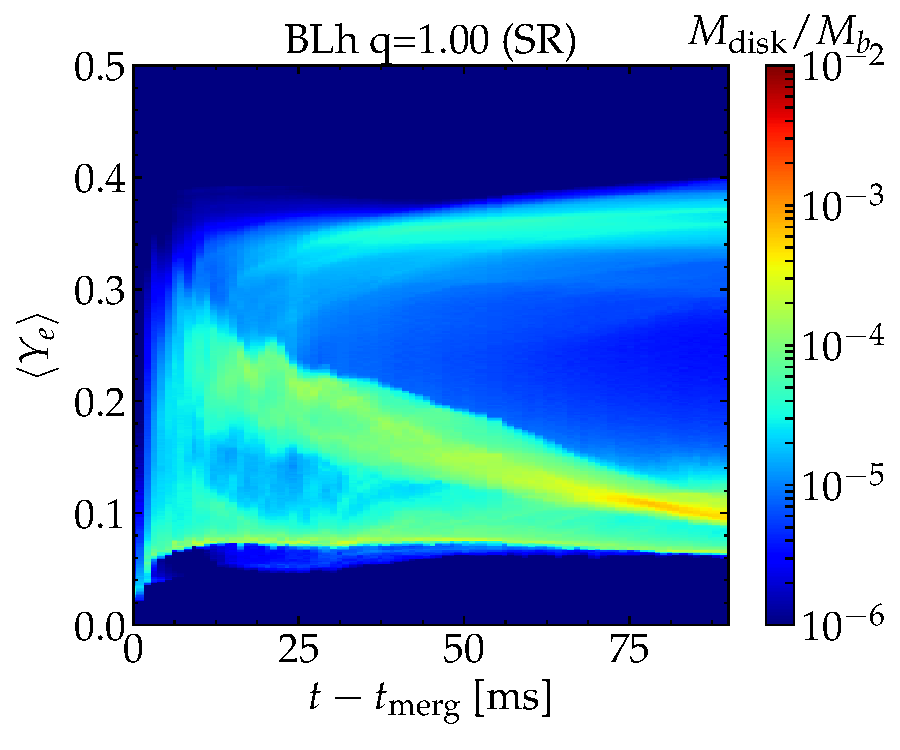
\includegraphics[width=0.49\textwidth]{disk/final_disk_timecorr_blh_q1_Lk.pdf}
    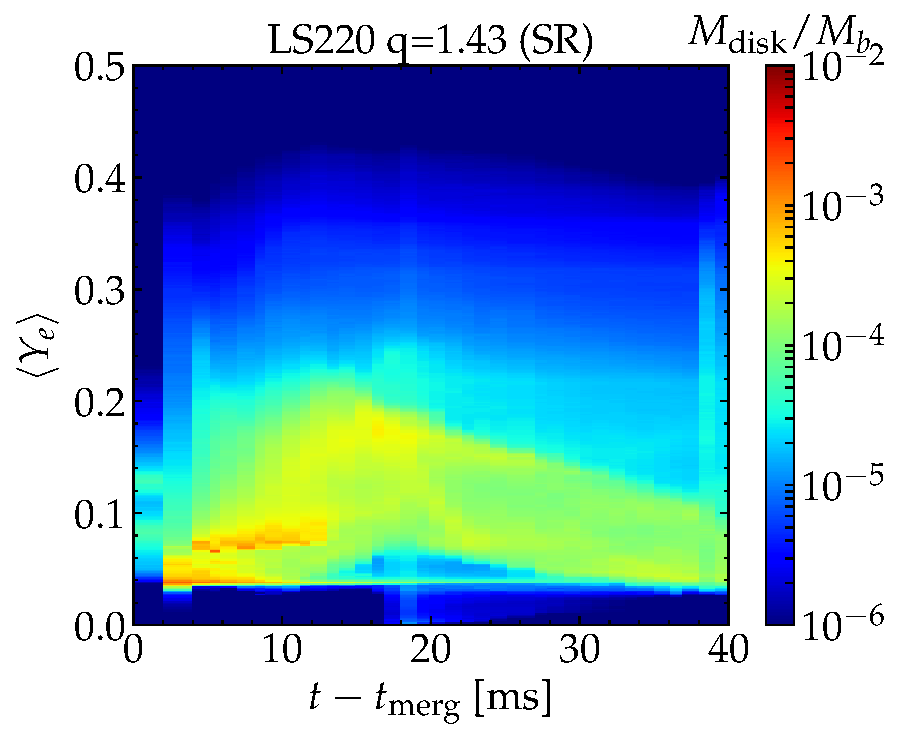
\includegraphics[width=0.49\textwidth]{disk/final_disk_timecorr_ls220_q14_LK.pdf}
    \caption{Evolution of the disk mass-averaged electron fraction with
        time for a long-lived (top) and a short-lived (bottom)
        remnant. The plot shows that with time the bulk of the disk lowers
        its $Y_e$ via cooling, while a small fraction in terms of mass
        gains a high $Y_e$, which relates to the highly 
        irradiated surface of the disk. Adopted from \citet{Nedora:2020pak}.
    }
    \label{fig:total_disk_time_corr_Ye_Blh_q1}
\end{figure}

\paragraph*{Evolution of disk properties}

%% Ye evolution
The evolution of the mass-weighted electron fraction for the model
BLh $q=1.00$, the model that is evolved till $\sim 90$~ms after merger, 
is shown on the top panel of Fig.~\ref{fig:total_disk_time_corr_Ye_Blh_q1}.
%% --- 
During the formation, shock and spiral waves raises the disk electron fraction to
$Y_e\sim0.25$. As the disk evolves, the bulk of its mass, shielded from neutrinos, 
(Fig. \ref{fig:slice:heating_hu}, density contours) 
returns to neutron-rich condition with $Y_e\lesssim0.1$. 
The outer part of the disk, however, is subjected to the 
strong neutrino irradiation and reaches $Y_e\sim0.4$ of a timescale of ${\sim}40$~ms.
%% Note that neutrinos in merger remnants decouple at $\rho\sim10^{11}$~$\gccm$ \citep{Endrizzi:2019trv}. 
Notably, the apparent gap in the $Y_e$ distribution if Fig.~\ref{fig:total_disk_time_corr_Ye_Blh_q1} at $\langle Y_e \rangle \simeq 0.15$ 
might not be of physical origin, but an artifact from the neutrino M0 scheme, 
that assumes neutrinos propagate along the radial directions
(see sec.NEUt.M0.SCHEME), that is not well suited for capturing the 
neutrino emission and reabsorption from the disk midplane.
%% ---
In case of a short-lived model LS220 $q=1.43$ model 
(lower panel of the Fig.~\ref{fig:total_disk_time_corr_Ye_Blh_q1})
the average electron fraction is lower, as there is no strong neutrino 
emitter. Additionally, the outskirts of the more compact disk remain 
at low electron fraction as the neutrino emitted by the disk itself 
are the only source of neutrinos. 

\paragraph*{Mass ejection on a long timescale}

As the disk expands and cools, the recombination of nucleons into 
alpha particles starts to take place.
The energy, released in recombination, might be sufficient for the outermost 
layers to become unbound, generating an outflow 
\citep{Beloborodov:2008nx,Lee:2009uc,Fernandez:2013tya}.
This processes however are expected to take place on a longer timescales,
that those that are simulated here.
On the $\sim100$~ms timescale, the outflows are driven by the neutrino heating, 
above the remnant, the so-called neutrino-driven wind 
(\nwind; \citealt{Dessart:2008zd,Perego:2014fma,Just:2014fka}),
and by the dynamical interactions between the \ac{MNS} 
remnant and the disk, the \swind{} \citep{Nedora:2019jhl}.
%% ---
We discuss the properties of the \nwind{} found in our simulations
in the section \red{sec.Ejecta.NuWind} and the properties of the 
\swind{} in the \red{sec.Ejecta.SWIND}.
%The \swind{} can have a mass up to
%a few $10^{-2}\,\Mo$ and velocities ${\sim}0.2$~c. The ejecta
%have electron fraction typically larger than ${\sim} 0.25$ since they are 
%partially reprocessed by hydrodynamic shocks in the expanding arms. 
%The \nwind{} is driven by neutrino heating above the remnant. It generates outflows
%with smaller masses ${\sim} 10^{-4}M_{\odot}$ and larger $Y_e$
%than the \swind{}. 
%Differently from \swind{} the mass flux of the \nwind{} in our simulations subsides 
%before the end of out simulations, due to rapid baryon loading of the 
%polar region.
%The \swind{} will be discussed in detail in Sec.~\ref{sec:spiralw}.
The effects of these outflows on the dynamical evolution of the remnant 
lies in the amount of mass and energy they can remove from the system.
Specifically, the \nwind{} have a typical mass of ${\sim} 10^{-4}\Msun$, 
while the \swind{} could remove $10^{-2}\,\Msun$ on a timescale of a $\sim100$~ms.

\begin{figure}[t]
    \centering 
    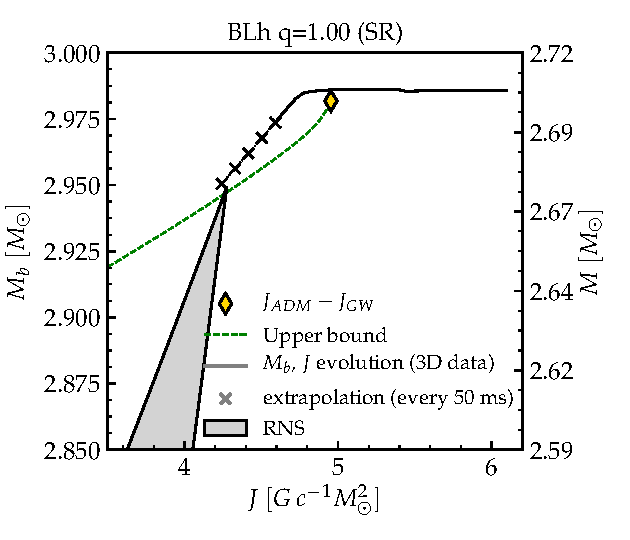
\includegraphics[width=0.49\textwidth]{ejecta_sec/secular_j_mb_RNS_blh.pdf}
    \caption{Baryon mass vs angular momentum diagram for the BLh $q=1$ remnant.
        The colored diamond marks the baryonic mass and angular momentum at the end
        of the dynamical gravitational-wave dominated phase.
        After the GW phase, the evolution is driven by the massive outflows.
        The solid black line is the $M_b$ and $J$ estimated from the 3D data
        integrals under the assumption of axisymmetry.
        The green dashed line is a conservative estimate
        of the mass ejection and a possible trajectory for the viscous
        evolution as estimated in \citet{Radice:2018xqa}. The crosses are
        a linear extrapolation in time of the solid black line. The gray
        shaded region is the region of stability of rigidly rotating NS equilibria.
        Adopted from \cite{Nedora:2020pak}
    }
    \label{fig:total_j_mb_rns_blh}
\end{figure}

To understand the remnant evolution on the timescales longer then the ones 
present here, requires ab-initio \ac{NR} simulations in $(3+1)D$ with compete physics.

Here we consider a BLh $q=1.00$ simulation, one of the longest runs we have performed.
After the merger, the \ac{MNS} remnant is born. With respect to the zero-temperature 
beta-equilibrium \ac{NS} configurations, the BLh $q=1.00$ 
remnant has an excess in baryon mass.
In the figure~\ref{fig:total_j_mb_rns_blh} we show the evolution of the 
total baryon mass, $M_b$, and total angular momentum, $J$, of the remnant.
As the total baryon mass is conserved (if there is no outflow), the early evolution 
of the remnant proceeds with $M_b=\text{const}$. The angular momentum is however 
lost by the remnant to emission of \acp{GW}. 
We evaluate the amount of angular momentum lost to \acp{GW} following the 
\citet{Damour:2011fu,Bernuzzi:2012ci,Bernuzzi:2015rla}.
\red{This has to be defined and noted that we use $\sim20$~ms postmerger mark
    and how exactly we compute all of it, the David's script
}
Substruct it from the initial data \ac{ADM} angular momentum we obtain the value 
that is left to the system after the \ac{GW} phase 
(the yellow marker on the Fig.~\ref{fig:total_j_mb_rns_blh}).
%% ---
Notably, after the \ac{GW} phase, the remnant still has an excess in angular momentum
in comparison with the rigidly rotating \ac{NS} configurations with the same baryon mass 
(gray triangular region in Fig.~\ref{fig:total_j_mb_rns_blh}).
We observe the same situation across all models \citep{Zappa:2017xba,Radice:2018xqa}.
\gray{
    On the angular momentum estimation:
    The radiated angular momentum (as well as energy) are computed from the 
    multipole loments $N_{lm}$ for the \ac{NR} complex "news function" at infinity. 
    The $J_{z;\text{rad}}(t)$ is computed as \citep{Damour:2011fu} 
    \begin{equation}
    \Delta J_{z\text{rad}}(t) \frac{1}{16}\sum_{l,m}^{l_{max}}\int_{t_0}^{t} dt' m \mathcal{L}[h_{lm}(t')(N_{lm}(t'))^*],
    \end{equation}
    where $h_{lm}$ is the multipolar metric waveform, 
    $N_{lm}(t) = dh_{lm}(t) / dt$, the news function, and $l_{max}=8$.
    The $J$ loss is metric dependent ($h$).
    The $h$ (strain???) is computed from $\Psi_4(t) = dN/dt = d^2h/dt^2$ by a 
    frequency-domain integration procedure with a low-frequency cut 
    $\omega_0 = 0.032/(m_1+m_2)$.
}
%% ---
The baryon mass of the remnant also exceeds maximum mass that a rigidly rotating 
equilibria could have.
Such remnant is generally referred to as a hypermassive neutron star (HMNS) following the 
nomenclature introduced for zero-temperature EOS equilibria \acp{NS} \citep{Baumgarte:1999cq}.
Such a remnant is expected to collapse to a BH. 
%% ---
However, a remnant can avoid the collapse by efficiently removing angular momentum
and mass and entering the rigidly rotating equilibria zone. 
%% ---
We compute the angular momentum and baryon mas evolution of the remnant, 
through volume integrals, assuming axisymmetry and evaluating the former using Eq.~\eqref{eq:method:ang_mom}, and the latter using the Eq.~\eqref{eq:method:mdisk}. 
The evolution of these two quantities is depicted with the black solid line if 
Fig.~\eqref{fig:total_j_mb_rns_blh}~\footnote{Note that the angular momentum estimated
    from the GW and from the integral of Eq.~\eqref{eq:method:ang_mom} assuming
    axisymmetry are compatible within the errors made in the latter estimate.
}.
We observed that after the \ac{GW} phase, the remnant continues to evolve, loosing the 
angular momentum together with the baryon mass. This is achieved through massive outflow,
the \swind{}. 
The extrapolation of the final trend of the mass and angular momentum loss shows, that 
if $\approx0.05\,\Msun$ ($\approx40$\% of the final disk at the end of simulation) is 
ejected, the \ac{MNS} remnant would approach the rigidly rotating equilibria region 
at the mass-shedding limit. Extrapolation indicates, that if the ejecta mass flux does 
not change, this would occur on a timescale of $\sim 300$~ms \pmerg{}.
Similar results are obtained with the conservative upper bound estimate on the 
evolution of the long-lived remnant (Eq.~$2$ in \citet{Radice:2018xqa}) (green dashed line in figure).
\red{WHAT the fuck is Keplerian limit, mass-shedding limit and rigidly rotating equilibria}
Additionally, while this simulation included the effects of turbulent viscosity on the
angular momentum transport, the ejecta could be further enhanced by the magnetic stresses 
\citep{Metzger:2006mw,Bucciantini:2011kx,Siegel:2017nub,Fernandez:2018kax,Ciolfi:2020hgg}.

Other simulations also produce a \ac{MNS} remnant with a similar evolutionary path. 
Models with DD2 \ac{EOS} however, are born with an excess in angular momentum, but not in 
baryon mass. They also evolve toward the rigidly rotating equilibria but slower.
Models with $q>1.00$ produce remnants that generally have larger excess in angular momentum 
and mass have how to shed a larger amount of mas to reach equilibrium configuration.
(\red{However we also show that these models tend to have stronger \swind{}, see sec.SPIRAL.WIND})
Overall, we estimate that for models with $q=1.00$ need to shed ${\sim}0.05\Msun$ while 
models with $q\eqsim 1.4$ need to remove $0.2\Msun$ to reach equilibrium configuration.



\section{Mass ejection in \ac{BNS} merger simulations}

%% \section{Results -- Mass Ejection}


Tidal interactions and shocks exerted on the \acp{NS} at merger trigger the ejection of material
on the dynamical timescale. This is the \ac{DE} \citep[\eg][]{Hotokezaka:2013b,Bauswein:2013yna,Radice:2016dwd,Radice:2018pdn}. 



\subsection{Dynamical Ejecta}


%% The mechanism behind the dynamical ejecta [radice:2018pnd]
Tidal interactions and shocks exerted on the \acp{NS} at merger trigger the ejection of material
on the dynamical timescale. This is the \ac{DE} \citep[\eg][]{Hotokezaka:2013b,Bauswein:2013yna,Radice:2016dwd,Radice:2018pdn}. 

\red{More on the genral mechanism tidal vs shocked}
The \ac{DE} is evaluated with the geodesic criterion introduced in Sec.~\ref{sec:method:analysis:ejecta}.

Describe shock vs tidal components 

\subsubsection{Overall properties of the \ac{DE}}


The novelty of the set of models discussed in this thesis with respect to the 
previous study by \citet{Radice:2018pdn} is that all models include the neutrino heating via M0 scheme 
(see Sec.\ref{sec:theory:neutrino}) in addition to the neutrino cooling and for most models the effects 
of subgrid turbulence (see Set.\ref{sec:theory:grles}) are included.
Meanwhile, models cover a significantly more narrow range in 
dimensionless tidal deformability, $\tilde{\Lambda}$, and mass ratio, motivated by the \GW{}.

We can qulitativly asses the effects of neutrino heating by comparing the overall properties 
of our model set and that of the \citet{Radice:2018pdn}.
Specifically, the neutrino absorption leads to not only an increase in average electron 
fraction but also to larger total ejected mass and velocity. The latter two would be 
crucial for the non-thermal, kilonova afterglow (see Sec.\red{sec:KilonovaAfterglow}).

The mass averaged over the simulations from Tab.~\ref{tab:sim} is 
$\overline{\amd} = (3.442 \pm 2.495)\times 10^{-3}\,M_{\odot}$ (where
hereafter we report also the standard deviation), while the same
quantity calculated for data of \cite{Radice:2018pdn} 
is $\overline{\md} = (1.352\pm 1.250)\times 10^{-3}\,\Msun$.
The mass-averaged terminal velocity of the dynamical ejecta 
ranges between $0.1$c and $0.3$c, and in a good agreement with 
\cite{Radice:2018pdn}.
The mass-averaged velocity, averaged over all the simulations, is 
$\overline{\avd} = (0.172\pm0.038)\,{\text{c}}$.

We find that in our set of models, there is a correlation of $\avd$ with the tidal parameter 
$\tilde{\Lambda}$: the higher the $\tilde{\Lambda}$ the lower the $\avd$.
This can be understood from the general mechanism of the \ac{DE},
that tells in mergers of binaries with $q=1.00$, the shocked component of the ejecta 
is the dominant. The strength of shocks increases as the \acp{NS} become more compact 
(with decreasing $\tilde{\Lambda}$) and hence collide at higher velocities~\footnote{Note that in the definition of prompt collapse we adopted, there is no shocked ejecta.}.
%% ---
For binaries with high mass ration, however, the tidal component of the \ac{DE} is dominant. 
The velocity of the latter also is smaller for larger $\tilde{\Lambda}$, as stars collide 
at slower velocities due to their larger radii. 
%% ---
The mass-averaged electron fraction, $\ayd$, of our models lies the range $(0.1, 0.3)$
with an averaged value among all models $\overline{\ayd} = 0.175 \pm 0.063$.
Notably, the \citet{Radice:2018pdn} reported a more narrow range, $(0.1, 0.2)$.
This is a clear effect of the neutrino absorption included in our models, that elevates 
the everal electron fraction of the \ac{DE} as it is being irradiated by neutrinos 
during the merger.
Notably, the $\ayd$ of our models is close to those obtained with M1 
scheme of \citet{Sekiguchi:2016bjd} and \citet{Vincent:2019kor}.
%% ---
The effect of subgrid turbulence on the dynamical ejecta properties however,
found rather week and comparible to the effects of finite grid distritization 
\citep{Bernuzzi:2020txg,Radice:2020ids}.

We find that the properties of the \ac{DE} depends on the \mr{} and on the 
\ac{EOS} softness that can be parameterized with $\tilde{\Lambda}$. 
We investigate in detail the statistical properties of our set of models as well as 
other \ac{NR} \ac{BNS} data sets available in the literature in 
section \ref{sec:ejecta_disk_statisitcs}.
\red{Link to the fitting data}



\subsection{Fast tail of the dynamical ejecta}
\red{To be filled when the Afterglow paper is on arxive}

%\begin{figure}[t]
%    \centering 
%    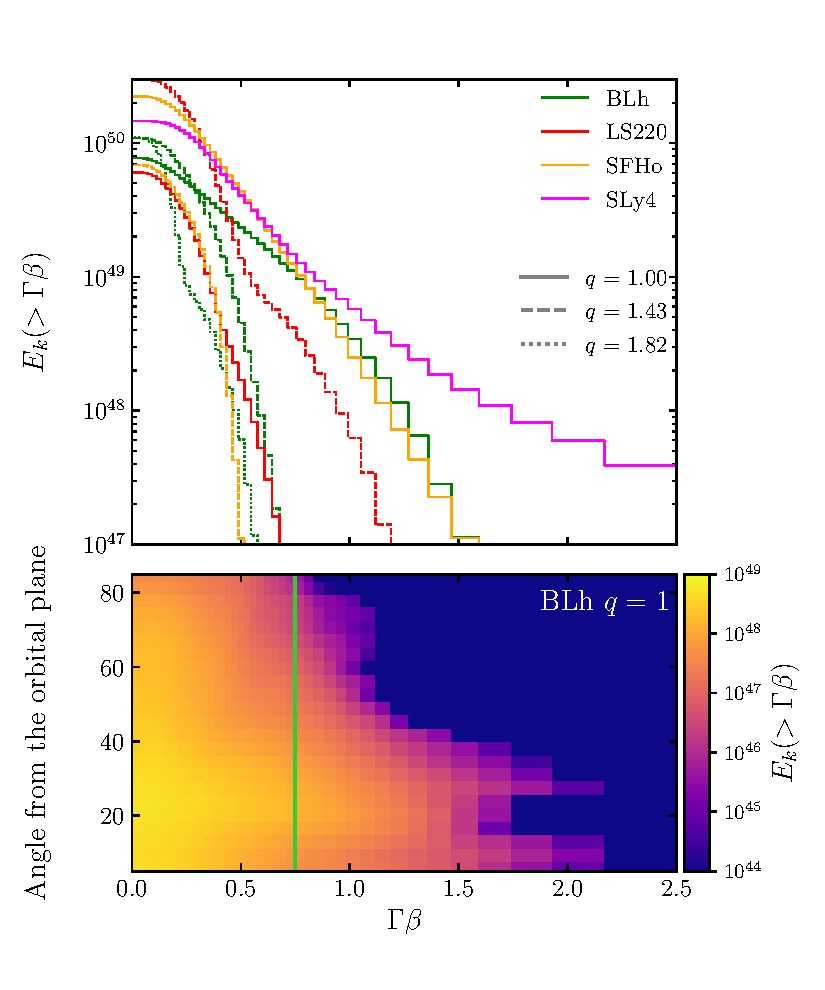
\includegraphics[width=0.49\textwidth]{./figs/kinetic_energy_struct_models.pdf}
%    \caption{
%        Total kinetic energy distribution for a selected set of models (\textit{top panel}) 
%        and angular distribution of kinetic energy for a BLh $q=1.00$ model (\textit{bottom panel}).
%        %% Also shown as a solid black line is the slow quasi-spherical model of \cite{Mooley:2017enz}.
%        The vertical light green line marks the $\upsilon_{\text{ej}}=0.6$.
%        The top panel shows that equal mass models have a more extend high energy tail,
%        while the bottom panel shows that the angular distribution of the ejecta is not 
%        uniform.
%        \red{Adopted from Nedora et al. (2021)}
%    } 
%    \label{fig:ejecta_vel_hist}
%\end{figure}
%
%The velocity distribution of \ac{DE} was found to include a very fast, 
%$\upsilon_{\text{ej}}\geq0.6$~c tail
%\cite{Piran:2012wd,Hotokezaka:2013b,Kyutoku:2012fv,Ishii:2018yjg,Hotokezaka:2018gmo,Radice:2018pdn}.
%%% ---
%The total mass of this tail was found to be dependent on the
%binary parameters and solution resolution,
%with an average $\sim 10^{-6}-10^{-5} M_{\odot}$.
%%% ---
%With respect to the fast tail origin, it can be divided into two main components 
%\citep{Radice:2018pdn}.
%The early component, that comprises the ejecta that is generated at the collisional interface 
%of two \acp{NS} of similar mass and directed primarily along the binary axes.
%And the late component that consist of matter that driven by the shock breakout from the ejecta 
%after the core bounce and confined mostly to the binary plane. 
%
%Among the simulations listed in \ref{tab:sim}, we select \red{XX} simulations 
%performed at standard resolution, and for which fast ejecta is found.
%%% ---
%Here we extract ejecta properties at the detector located at 
%$R=300G/c^2M_{\odot}\approxeq443$~km, from the merger, in agreement with \citet{Radice:2018pdn}.
%
%The mean value of the fast tail mass is
%
%\be\label{eq:ejecta:dyn:avg:M}
%\red{ \overline{\amd}(\upsilon>0.6) = (2.50 \pm 4.23)\times 10^{-5}M_{\odot}\ , }
%\ee
%
%where the standard deviation is also reported as an error.


%% ------------------ 
%% Note that the geodesic criterion above neglects the fluid's pressure and might
%% underestimate the ejecta mass. The Bernoulli criterion assumes that the (test
%% fluid) flow is stationary, so that there is a pressure gradient that can
%% further push the ejecta.  We find that both criteria predict dynamical
%% ejecta masses that are practically indistiguishable and well within the numerical uncertainties \citep{Bernuzzi:2020txg} if applied to extraction spheres at large coordinate radii; 
%% differences between the two criteria are instead present if they are applied to
%% matter volumes \citep[cf.][]{Kastaun:2014fna}.


\subsection{Spiral-wave wind}

\label{sec:spiralw}


\begin{figure*}[t]
    \centering 
    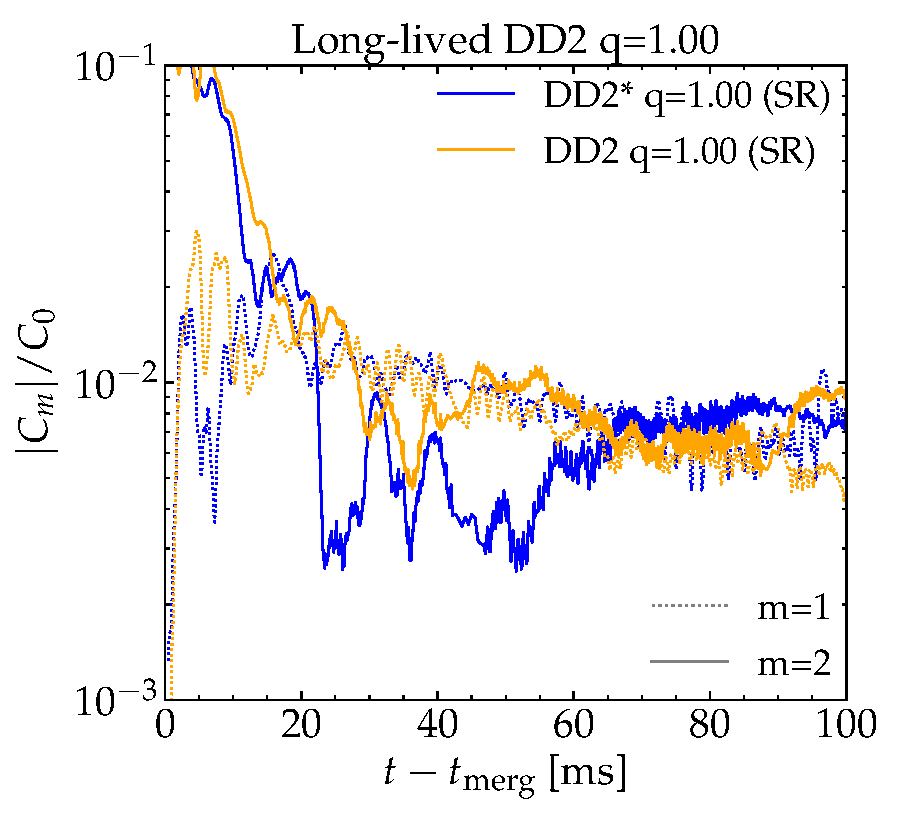
\includegraphics[width=0.49\textwidth]{remnant/dens_modes/modes_rho_dd2.pdf}
    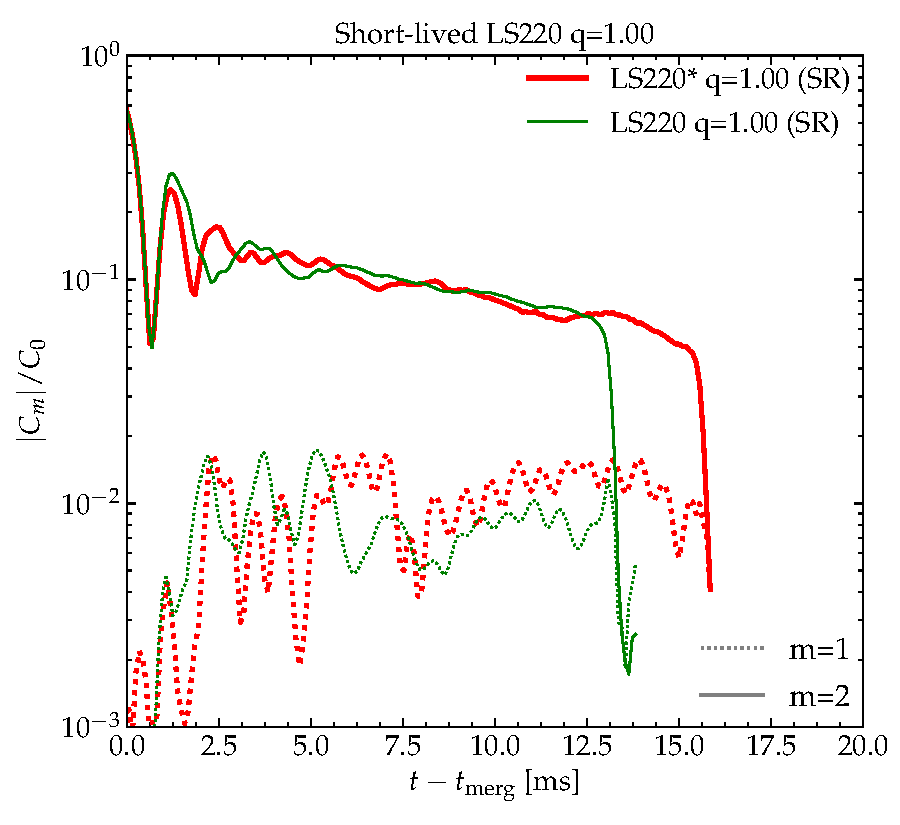
\includegraphics[width=0.49\textwidth]{remnant/dens_modes/modes_rho_ls220.pdf}
    \caption{Modes analysis for exemplary equal-mass long-live and short-lived
        remnants. The evolution of the $m=2$ and the $m=1$ monitored by
        Eq.~\eqref{eq:modes} is shown for the DD2 and LS220 remnant with and
        without turbulent viscosity. The $m=2$ mode in the long-lived
        remnant is strongly damped by the emission of gravitational
        radiation and becomes comparable to the $m=1$ mode on a timescale of
        ${\gtrsim}20\,$ms. Turbulent viscosity sustain the $m=2$ mode for
        a longer period. The $m=2$ mode is instead dominant to collapse in
        the short-lived remnant.
        (Adopted from \cite{Nedora:2020pak})
    }
    \label{fig:dens_modes}
\end{figure*}

Here we discuss the dynamics of spiral waves and the associated outflow, the \ac{SWW}.


\subsubsection{Remnant \& disk dynamics}


The hydrodynamical modes of the \ac{MNS} remnant are computed following the 
method described in Sec.\ref{sec:method:HDmodes}. 
The mode analysis is shown in the Fig.\ref{fig:dens_modes} for two representative 
simulations, the short-lived LS220 $q=1.00$ and the long-lived DD2 $q=1.00$.
The newly born \ac{MNS} remnant is not axisymmetric, displaying characteristic 
spiral arms, extending outwards from the shock interface of the collided cores 
\citep{Shibata:1999wm,Shibata:2006nm,Bernuzzi:2013rza,Kastaun:2014fna,East:2015vix,Paschalidis:2015mla,Radice:2016gym,Lehner:2016wjg}.
The bar-shaped, $m=2$ modes is the dominant one early in \pmerg{}, while the 
one-armed spiral $m=1$ modes stars to dominate in the late evolution 
\citep{East:2015vix,Paschalidis:2015mla,Radice:2016gym,Lehner:2016wjg,Bernuzzi:2013rza,Kastaun:2014fna}.
Indeed, the $m=2$ mode remains the dominant one until $\sim15-20$~ms \pmerg{}. 
After that, the LS220 $q=1.00$ model forms a \ac{BH}. 
In the DD2 $q=1.00$ model, however, the $m=1$ mode becomes comparable with $m=1$ 
throughout the remainder of the evolution, while the $m=2$ mode efficiently dissipates 
through \ac{GW} emission \citep{Bernuzzi:2015opx,Radice:2016gym}.
%% ---
We find that the magnitude of the $m=1$ mode increases with the binary \mr{}.
For instance the largest $C_{m=1}$ are found in BLh $q=1.43$ and LS220 $q=1.22$.
Stronger $m=1$ leads to more large \ac{SWW} mass flux.
The dependency of the $C_{m=2}$ on \mr{} however is not clear. 
This is in agreement with what reported by \citet{Lehner:2016wjg}.

Formation of the spiral arms is a generic hydrodynamic effect, that was identified 
in the \ac{NR} simulations with polytropic \ac{EOS} 
\citep{Bernuzzi:2013rza,Radice:2016gym}.
However, the evolution of these arms and quantitative behaviour of hydrodynamic
modes depends on the physics input. 
In the Fig.~\ref{fig:dens_modes} we show that the turbulent viscosity in the 
DD2 $q=1.00$ remnant stabilizes the $m=2$ mode, enhancing the angular momentum 
transport into the disk.
The $m=2$ mode, however, remains largely unaffected by the turbulent viscosity.
Similarly, the models' evolution in the LS220 $q=1.00$ is too short, for the 
subgrid turbulence to become important.

We compute the angular momentum of the \ac{MNS} remnant following the method,
discussed in Sec.\ref{sec:method:angmom}, where the remnant is distinguished 
from the disk on the basis of the rest mass density $\rho=10^{13}$~\gcm{} 
(see Sec.\ref{sec:method:diskdef}).
We find that for a long-lived rmnant 
on a timescale of $\sim20$~ms, about half of the total angular momentum 
of the \ac{MNS} remnant is transferred into the disk. 
%% [ from shibata review ]
This is a consequence of the fact that the remnant \ac{MNS} is strongly deformed 
after merger and gravitational torque on the surrounding matter, 
that allows for a rapid angular momentum transport.
%% ---
After, the remnant settles on quasi-stationary evolution path 
(see Sec.~\ref{sec:bns_dynsmics_overview}).

Following the disk and remnant mass evolution we observe, that the spiral 
density modes inject ${\sim}0.1-0.4\,\Msun$ of baryon mass into the disk during the 
first ${\sim}20$ms. 
The mass injection appears to be stronger for stiffer \acp{EOS}. 
With respect to the \mr{}, the higher $q$ binaries form a larger disc 
(see BLh* $q=1.82$ and LS220* $q=1.43$ on the Fig.~\ref{fig:disk_mass_evo}).

\begin{figure}[t]
    \centering 
    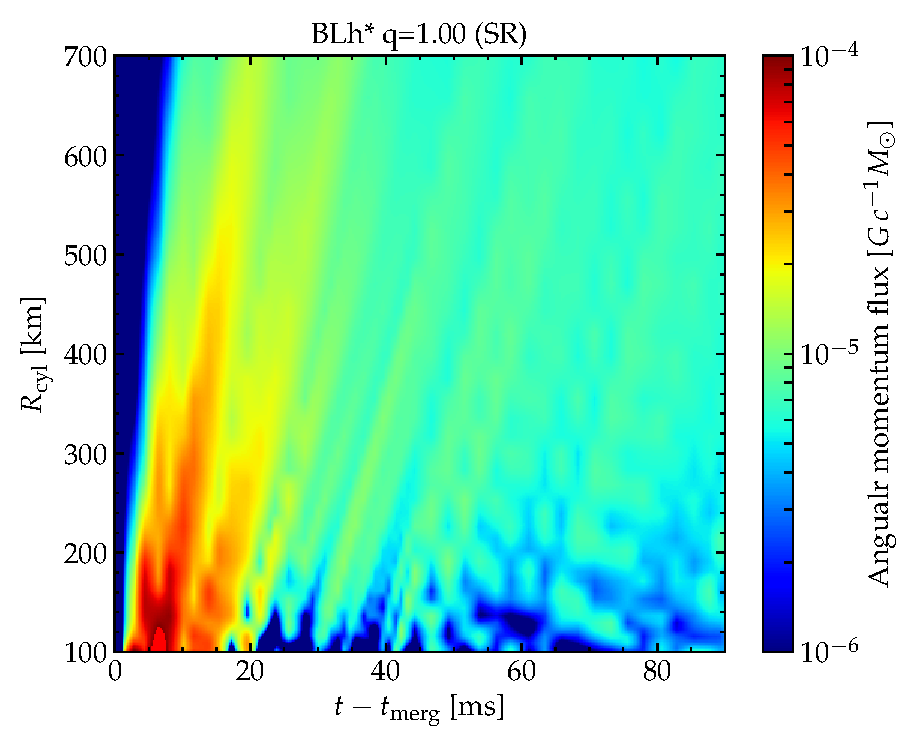
\includegraphics[width=0.49\textwidth]{remnant/evol_jflux_2d_BLh_M13651365_M0_SR_R1.pdf}
    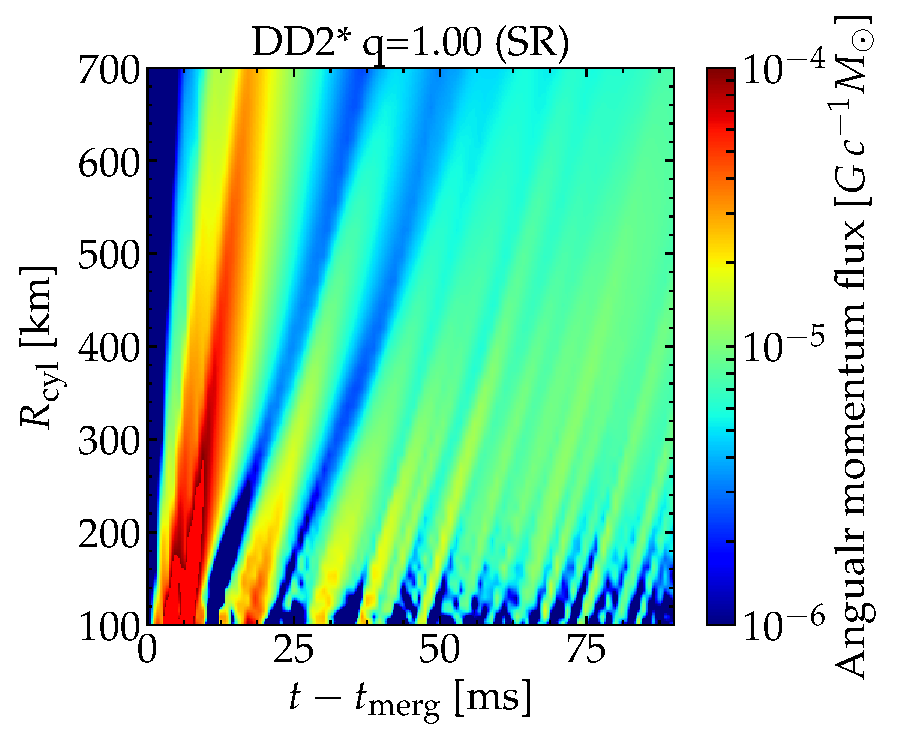
\includegraphics[width=0.49\textwidth]{remnant/evol_jflux_2d_DD2_M13641364_M0_SR_R1.pdf}
    \caption{Angular momentum flux through consecutive cylindrical
        surfaces identified by cylindrical radii from $R_{\text{cyl}}=100$ to $R_{\text{cyl}}=500$. The
        plot shows the angular momentum transport into the disk.
        Adapted from \citet{Nedora:2020pak}
    }
    \label{fig:disk_ang_mom_flux_map_blh_q1}
\end{figure}

In the Fig.~\ref{fig:disk_ang_mom_flux_map_blh_q1} we show how the 
angular momentum is being transported from the \ac{MNS} remnant into the disk
in two long-lived models with turbulent viscosity, DD2* $q=1.00$ and BLh $q=1.00$.
The angular momentum is transported via spiral waves that correspond do the 
hydrodynamic models, $m=1$ and $m=2$ discussed above.
We observer, that in the model with more stiff DD2 \ac{EOS},
the fist wave is stronger. Notably, the DD2* $q=1.00$ model 
also has a more massive disk.
%% --- 
Further, the evolution of the disk-remnant interactions 
after $\sim20$~ms \pmerg{} is different for two models. 
While the model with DD2 \ac{EOS} stops shedding mass into 
its disk and starts slowly accreting, the model with BLh \ac{EOS} continues to shed mass into the disk
(see Fig.~\ref{fig:disk_mass_evo} and discussion in
Sec.~\ref{sec:bns_dynsmics_overview})
The latter is caused by the strong angular momentum flux \red{actually the plot shows, that it is not}, emanating 
from the \ac{MNS} remnant and by the larger temperatures, 
that reached in the model with the BLh \ac{EOS}.
Larger temperatures leads to lower rotational frequency 
at which the mass shedding occurs \citep{Kaplan:2013wra}. 

The subgrid turbulence enhances the angular momentum transport. However more simulations of long-lived 
\ac{MNS} remnants are needed to asses the effects of the 
subgrid turbulence and \mr{} systematically. 

\begin{figure}[t]
    \centering 
    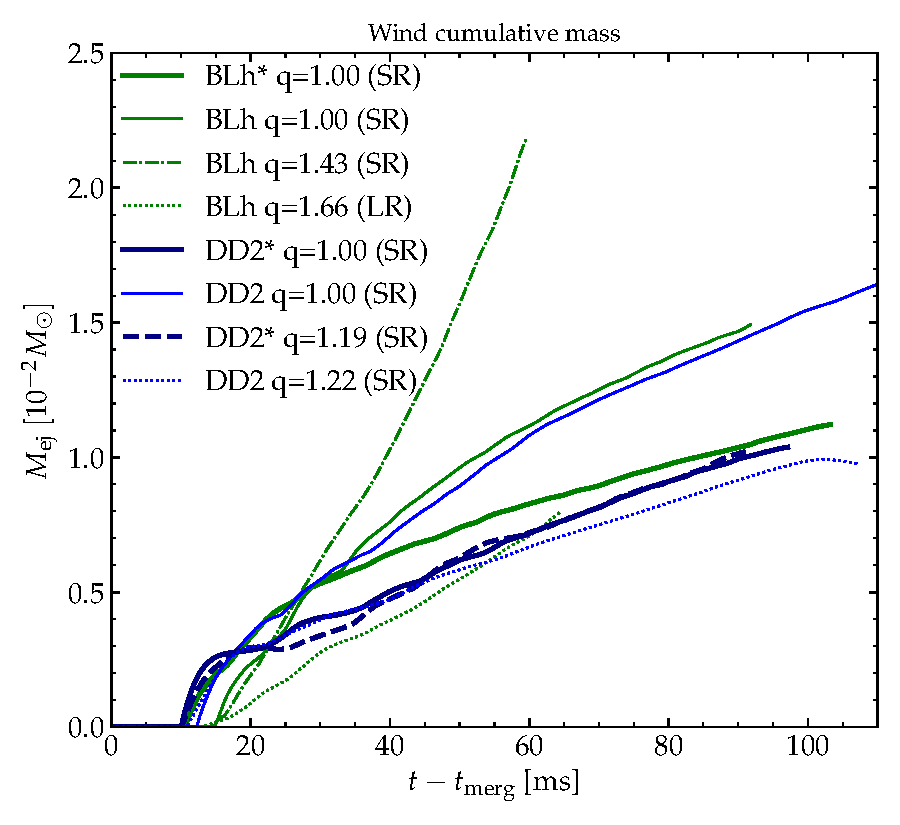
\includegraphics[width=0.50\textwidth]{ejecta_postdyn/wind_mass_flux.pdf}
    \caption{Cumulative mass of the \swind{} from long-lived
        remnants. The wind persists on timescales of $\O(100)\,$~ms with
        mass fluxes ${\sim}0.33-1.23\,\Msun/s$.
        Adapted from \citet{Nedora:2020pak}.
    }
    \label{fig:mej:bern}
\end{figure}

\begin{figure*}[t]
    \centering 
    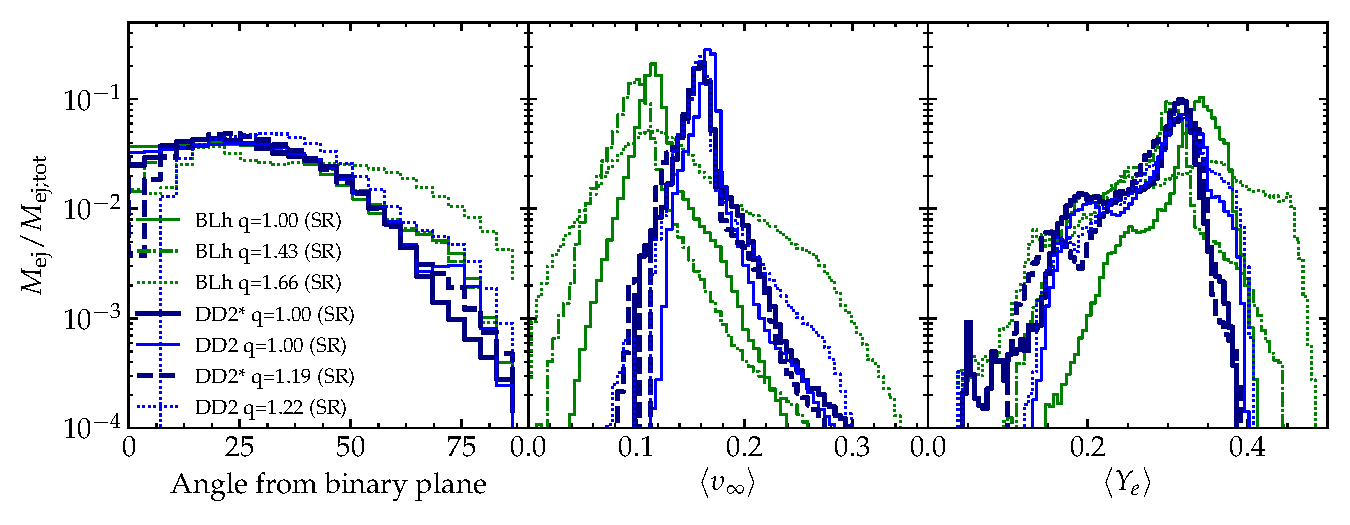
\includegraphics[width=0.99\textwidth]{ejecta_postdyn/wind_hists_shared.pdf}
    \caption{Mass-averaged histograms of the \swind{} for a selected
        subset of long-lived remnant. From left to right: ejecta angular
        distribution, ejecta terminal velocity and electron
        fraction. Remnants from more asymmetric binaries produce winds
        with broader angular distribution.
        The \swind{} from the DD2 EOS remnants has larger velocities
        then the winds from the softer BLh EOS. The electron fraction
        peaks at ${\sim}0.3$ and it is distributed from $0.1$ to $0.4$.
        Adapted from \citet{Nedora:2020pak}.
    }
    %
    \label{fig:ejecta:bern:hist}
\end{figure*}

\begin{figure}[t]
    \centering
    %% 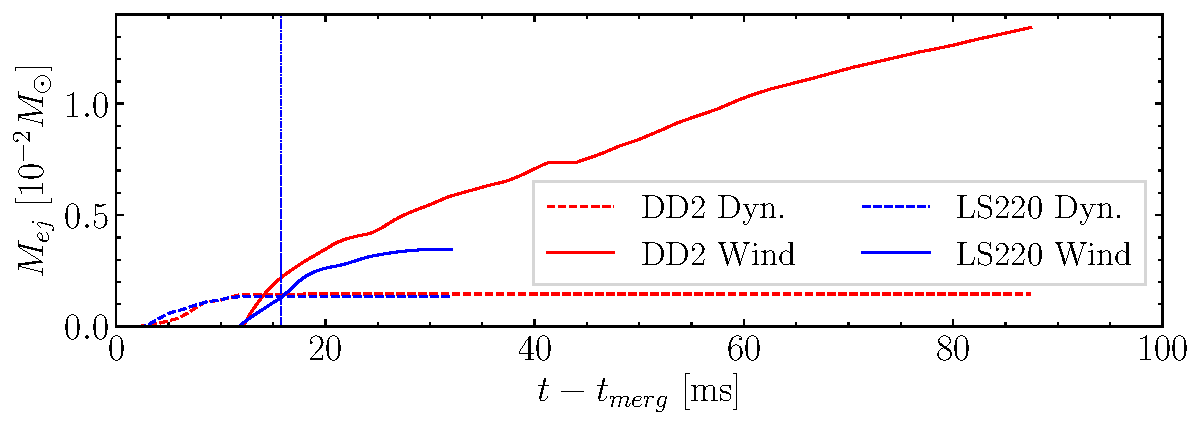
\includegraphics[width=0.49\textwidth]{ejecta_postdyn/ejecta_profiles_dd2_ls220_long.pdf}
    %% 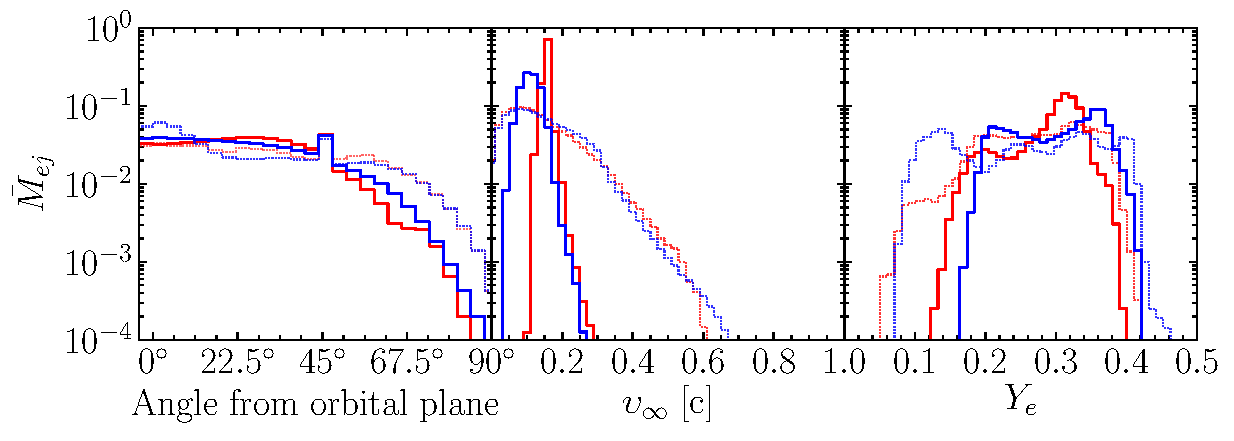
\includegraphics[width=0.49\textwidth]{ejecta_postdyn/hist_1D_dd2_ls220_long.pdf}
    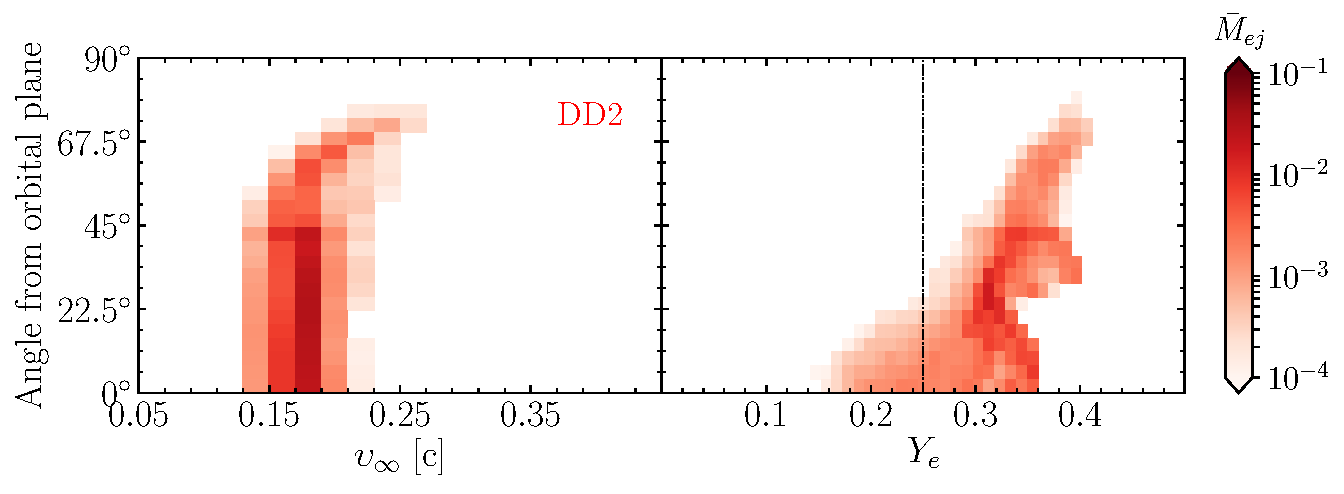
\includegraphics[width=0.99\textwidth]{ejecta_postdyn/corr_dd2.pdf}
    \caption{Properties of the \ac{SWW} and dynamical ejecta
        computed form the simulations with turbulent viscosity.
        %
        Top: evolution of unbound mass for dynamical ejecta
        (dashed lines)
        and \ac{SWW}
        (solid lines). $t=0$ marks the moment of merger, the vertical
        line marks the collapse time of the LS220 BNS.
        %
        Middle: mass histograms for the angular (left), velocity (center) and electron
        fraction (right) distributions.
        Bottom: angular distribution and composition of the \ac{SWW}
        for DD2.
        %
        Note the $\bar{M}_{ej}$ in the middle and bottom panels is normalized to one.
        (Adapted from \citet{Nedora:2019jhl})
    }
    \label{fig:ej_properties}
    
\end{figure}

%% --------------------------------
%% TAB WIND SUMMARY
\begin{sidewaystable}
%\begin{table*}[t]
  \centering
  \captionsetup{width=1.0\linewidth}
  \caption{%
    Summary table of the \swind{} properties of long-lived remnants. The columns contain
    the following information, starting from the left. Equation of
    state, mass-ratio, available resolutions,
    inclusion of subgrid turbulence, time of the
    simulation end, mass of the
    \swind{}, mass-loss rate via \swind, mass-averaged electron fracton, terminal
    velocity and, finally, RMS angle for \swind{}. For these four
    quantities we give the mean value among the resolutions and
    one-sigma deviations. For binaries for which only one
    resolution is present, the error is assumed to be $20\%$ of the value.
    (Adapted from \cite{Nedora:2020pak}).
    }
  \label{tab:spiralwavewind}
  \begin{tabular}{c c c c c c c c c c}
    \hline\hline
    EOS & $q$ & Resolution & GRLES & $t_{\text{end}}$ & $\amw$ & $\amw/\Delta t$ & $\ayw$ & $\avw$ & $\langle \theta_{\text{ej}}^{\text{w}} \rangle$ \\
    &   &   &   & [ms] & $[10^{-2} M_{\odot}]$ & $[M_{\odot}/s]$ &   & $[c]$ &   \\ 
    \hline
    \hline
    BLh & 1.00 & \texttt{SR HR LR} & \cmark & $43.3$ $91.8$ $23.1$ & $0.39^{+0.07} _{-0.07} $ & $0.70^{+0.32} _{-0.32} $ & $0.31^{+0.01} _{-0.01} $ & $0.12^{+0.01} _{-0.01} $ & $27.06^{+2.61} _{-2.61} $ \\
    BLh & 1.00 & \texttt{SR} & \xmark & $ $ $103.2$ $ $ & $1.12^{+0.57} _{-0.57} $ & $1.07^{+0.21} _{-0.21} $ & $0.34^{+0.01} _{-0.01} $ & $0.12^{+0.02} _{-0.02} $ & $15.72^{+2.00} _{-2.00} $ \\
    \hline
    BLh & 1.18 & \texttt{LR} & \cmark & $69.4$ $ $ $ $ & $1.28^{+0.64} _{-0.64} $ & $1.23^{+0.25} _{-0.25} $ & $0.33^{+0.01} _{-0.01} $ & $0.11^{+0.02} _{-0.02} $ & $14.98^{+2.00} _{-2.00} $ \\
    \hline
    BLh & 1.43 & \texttt{LR SR} & \cmark & $35.1$ $59.6$ $ $ & $0.75^{+0.18} _{-0.18} $ & $1.06^{+0.67} _{-0.67} $ & $0.27^{+0.01} _{-0.01} $ & $0.09^{+0.01} _{-0.01} $ & $19.43^{+2.22} _{-2.22} $ \\
    \hline
    BLh & 1.54 & \texttt{LR} & \cmark & $45.8$ $ $ $ $ & $0.63^{+0.32} _{-0.32} $ & $0.44^{+0.09} _{-0.09} $ & $0.32^{+0.01} _{-0.01} $ & $0.10^{+0.02} _{-0.02} $ & $21.46^{+2.00} _{-2.00} $ \\
    \hline
    BLh & 1.66 & \texttt{LR SR} & \cmark & $64.6$ $20.1$ $ $ & $0.12^{+0.09} _{-0.09} $ & $0.37^{+0.34} _{-0.34} $ & $0.33^{+0.05} _{-0.05} $ & $0.13^{+0.01} _{-0.01} $ & $52.08^{+20.89} _{-20.89} $ \\
    \hline
    \hline
    DD2 & 1.00 & \texttt{LR SR HR} & \cmark & $123.0$ $113.0$ $74.4$ & $1.25^{+0.14} _{-0.14} $ & $1.30^{+0.19} _{-0.19} $ & $0.30^{+0.01} _{-0.01} $ & $0.17^{+0.00} _{-0.00} $ & $14.88^{+0.87} _{-0.87} $ \\
    \hline
    DD2 & 1.20 & \texttt{LR SR HR} & \xmark & $37.3$ $91.0$ $55.2$ & $0.48^{+0.09} _{-0.09} $ & $0.74^{+0.24} _{-0.24} $ & $0.26^{+0.01} _{-0.01} $ & $0.15^{+0.00} _{-0.00} $ & $24.54^{+2.23} _{-2.23} $ \\
    \hline
    DD2 & 1.43 & \texttt{LR SR} & \cmark & $37.7$ $62.0$ $ $ & $0.60^{+0.02} _{-0.02} $ & $0.51^{+0.06} _{-0.06} $ & $0.23^{+0.12} _{-0.12} $ & $0.16^{+0.00} _{-0.00} $ & $21.74^{+0.03} _{-0.03} $ \\
    \hline
    \hline
    SFHo & 1.43 & \texttt{SR} & \cmark & $ $ $46.5$ $ $ & $0.58^{+0.30} _{-0.30} $ & $0.43^{+0.09} _{-0.09} $ & $0.31^{+0.01} _{-0.01} $ & $0.17^{+0.02} _{-0.02} $ & $22.67^{+2.00} _{-2.00} $ \\
    \hline
    \hline
    SLy4 & 1.43 & \texttt{SR} & \cmark & $ $ $40.3$ $ $ & $0.53^{+0.27} _{-0.27} $ & $0.38^{+0.08} _{-0.08} $ & $0.29^{+0.01} _{-0.01} $ & $0.18^{+0.02} _{-0.02} $ & $23.52^{+2.00} _{-2.00} $ \\
    \hline\hline
\end{tabular}
%\end{table*}
\end{sidewaystable}

%% --------------------------------


\subsubsection{Properties of the \swind{}}

\gray{
    %% From Letter
    The long lived NS remnant (DD2) develops a \ac{SWW} more massive than the dynamical ejecta,
    as shown also in Fig.~\ref{fig:ej_properties}.
    The \ac{SWW} mass is larger the longer the remnant survives and 
    the more massive the disks are. It continues as long as as the 
    remnant does not collapse and the spiral modes persist.
    Thus, binary mass asymetry can enhance the \ac{SWW}
    as we find in simulations discussed elsewhere [In Prep.].
    The inclusion of turbulent viscosity alters all the ejecta masses with an
    additional component and, for the viscosity parametrization we
    have considered, it enhances the DD2 \ac{SWW} mass by ${\sim}25$\%.
    %
    The viscosity effect is larger than resolution effects.
    Comparing data at different grid resolutions we find that the
    largest variation is in the wind mass. The relative variation
    of mass from data pairs at increasing resolutions is ${\sim}+15\%$
    (LR-SR) and ${\sim}+8\%$ (SR-HR). Hence, finite grid effects tend to
    increase mass. A similar analysis on the average electronfraction
    and velocity indicate variations below $4\%$.
    % 
    The \ac{SWW} has an angular distribution of mass similar to the
    dynamical ejecta with material mostly confined to the orbital plane,
    as shown by the histograms in Fig.~\ref{fig:ej_properties}.
    On the contrary, the velocity profiles show a drastic difference
    between the two ejecta components. While the dynamical ejecta has a
    broad velocity distribution \citep{Hotokezaka:2012ze,Bauswein:2013yna,Radice:2018pdn}, the 
    \ac{SWW} velocity is narrowly distributed around  
    $0.2$c in the case of a long-lived remnant (DD2).
    The \ac{SWW} from the short-lived
    remnant (LS220) has a broader velocity distribution extending down to
    $0.1$c.
    This is due to the spiral-wave shutting down and the disk
    transition to a more steady accretion. As a consequence, the \ac{SWW}
    ceases but ejecta continue as a slower disc wind driven
    by nuclear recombination solely.
    The electron fraction of the \ac{SWW} has a
    narrower distribution than the dynamical ejecta in both
    cases. But because disks around NS remnants are less compact, 
    colder, and optically thicker than those around black
    holes~\citep{Perego:2019adq}, the outer layers of the DD2 disk have a 
    lower $Y_e$ than the LS220 disk and so does the \ac{SWW} coming from
    those layers.
    While the \ac{SWW} is generic in its hydrodynamics origin, the
    quantification of its properties relies on the accurate microphysics and
    neutrino treatment in our simulations.
}


Density waves, propagating outwards through the disk induce the outflow, the \ac{SWW} 
\citep{Nedora:2019jhl}.

\red{HERE THE LETTER STUFF COULD GO}

The \ac{SWW} is estimated following the Bernoulli criterion as described in 
the Sec.~\ref{ec:method:analysis}. 
We start to follow the \ac{SWW} after the \ac{DE} has saturated. 

We report the overall properties of the \ac{SWW} for all the models with the 
long-lived \ac{MNS} remnant that were also evolved for a sufficiently long time 
in the Tab.~\ref{tab:spiralwavewind}. 
The time evolution of the total mass of the \ac{SWW} is shown in the Fig.~\ref{fig:mej:bern}.
We observe that in all simulations \acp{SWW} persists till end without saturation.
This is because the outflow is driven by the angular momentum and mass transport 
induced by the dynamical instabilities in the remnant, the $m=1,2$ modes, discussed 
above. And as the $m=1$ modes are not efficiently damped \citep{Paschalidis:2015mla,Radice:2016gym,Lehner:2016wjg,East:2016zvv},
the \ac{SWW} could theoretically continue until the system collapses to a \ac{BH} 
or reaches the equilibrium (Sec.~\ref{sec:bns_dynsmics_overview}).

The strongest \ac{SWW} is found in binaries with $q>1$, such as 
$q=1.67$ and LS220 $q=\red{1.4}$. 
With the mass-loss rate ${\sim}0.5\, \Msun/{\text{s}}$, these models can eject 
${\sim}0.02\,\Msun$ within ${\sim}50$~ms of \pmerg{} evolution.
We find that as the \ac{EOS} becomes softer, lower \mr{} is needed to achieve high 
mass flux. For instance, the \ac{SWW} mass flux for BLh* $q=1.66$ is achieved by the 
model LS220* with $q=1.22$. 
A possible explanation for this is that the models with softer \ac{EOS} have stronger 
$m=1$ modes in the remnant (see Sec. \ref{sec:remdisk}).
When \ac{MNS} remnant collapses to a \ac{BH} and the mechanism that injects angular 
momentum into the disk shuts down, the \ac{SWW} mass flux subsides. 
Thus, the total ejected mass via \ac{SWW} is directly related  o the lifetime of the 
\ac{MNS} remnant, an addition to the binary parameters, \ac{EOS} and \mr{}.

The \ac{SWW} mass flux depends on the disk configuration, as more extended disks 
have outer layers that are less gravitationally bound. In turn, the disk 
configuration is dependent on the thermal effects. Higher temperature leads to 
stronger thermal pressure that increases the disk size. 
However, the dependency of the \ac{SWW} mass flux on the stiffness of the \ac{EOS} 
appears to be stronger, as the stiffer \ac{EOS} leads to a more massive disk 
(Sec.~\ref{sec:overview}). More simulations with longer postmerger evolution are needed 
to make a quantitative assessment. 
Overall the \swind{} from the long-lived remnant has a mass flux $\geq 0.4\, \Msun/{\text{s}}$.

We find that the properties of the \ac{SWW} depend only weakly on the binary parameters,
\mr{} and \ac{EOS}.The mass-histograms of the wind angular distribution, velocity and 
electron fraction are displayed in Fig.~\ref{fig:ejecta:bern:hist}. 
The angular distribution of the \ac{SWW} is similar to that of the \ac{DE}. The ejecta 
has a broad distribution around the binary plane.
The \ac{SWW} has a high average electron fraction, with the overall 
broad distribution of $0.1\lesssim \ayw\lesssim0.4$ that peaks at ${\sim}0.35$.
The low electron fraction material originates primarily at early times, when the 
material did not have enough time to be processed by neutrinos and before the 
outflow reaches quasi-steady state.
The \ac{SWW} average velocity is higher for stiffer \ac{EOS}, with the peak 
of the distribution laying between ${\sim}0.1\,$c and ${\sim}0.2\,$c.
However, more simulations of the \ac{MNS} remnants long-term evolution are 
required to confirm and quantitatively investigate this trend.
However, if it is indeed a generic feature, then it might imply 
an EOS dependent distinct feature in the electromagnetic counterpart. 
In particular, the observation of a fast blue kN given by the \swind{}
should be associated to a stiff EOS.

%% It is however expected, that as the system becomes more stationary and larger part 
%% of the disk accrets on the \ac{MNS} the outflow should subside. 


\subsection{\nwind{}}

\begin{figure*}[t]
    \centering 
    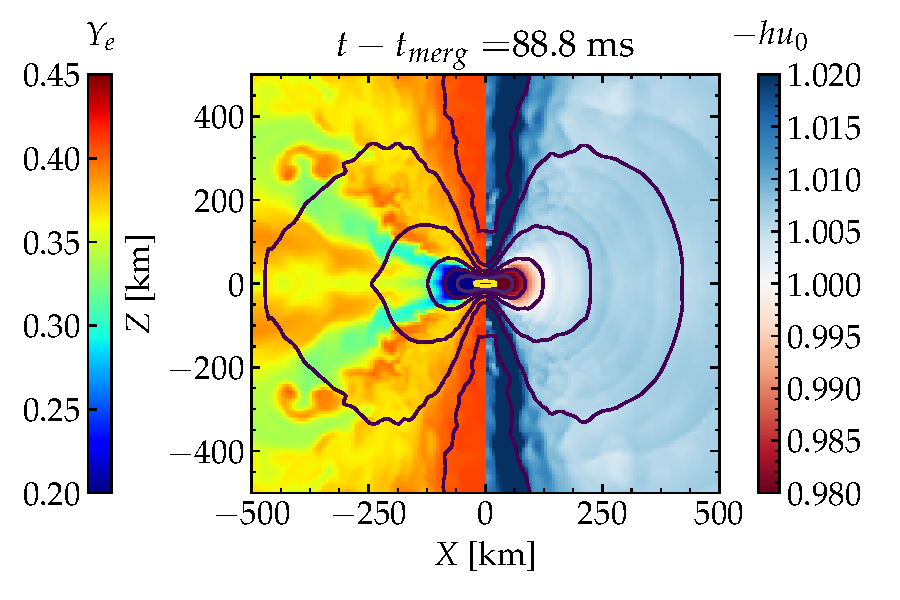
\includegraphics[width=0.49\textwidth]{slices/slice_xz_ye_hu_1.pdf}
    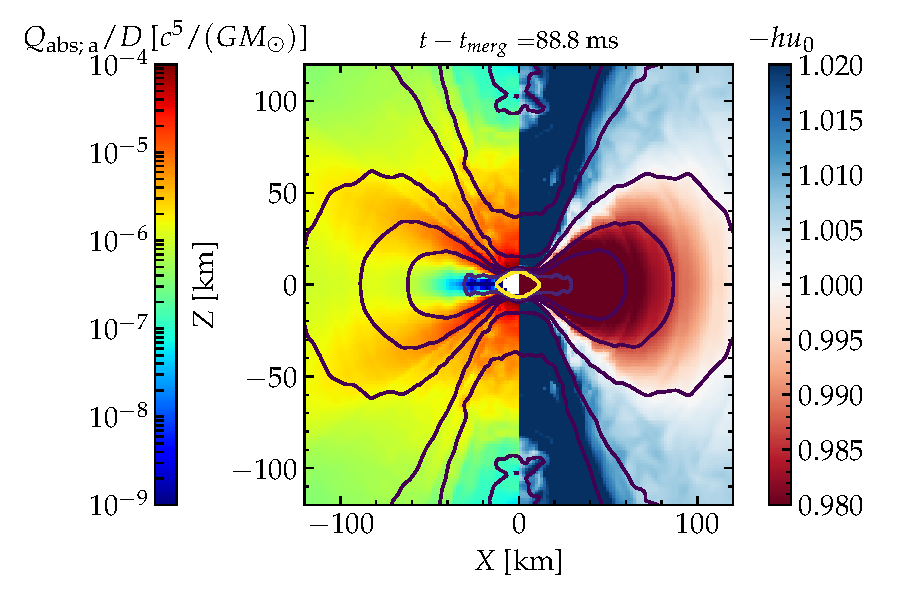
\includegraphics[width=0.49\textwidth]{slices/slice_xz_abs_energy_hu_3.pdf}
    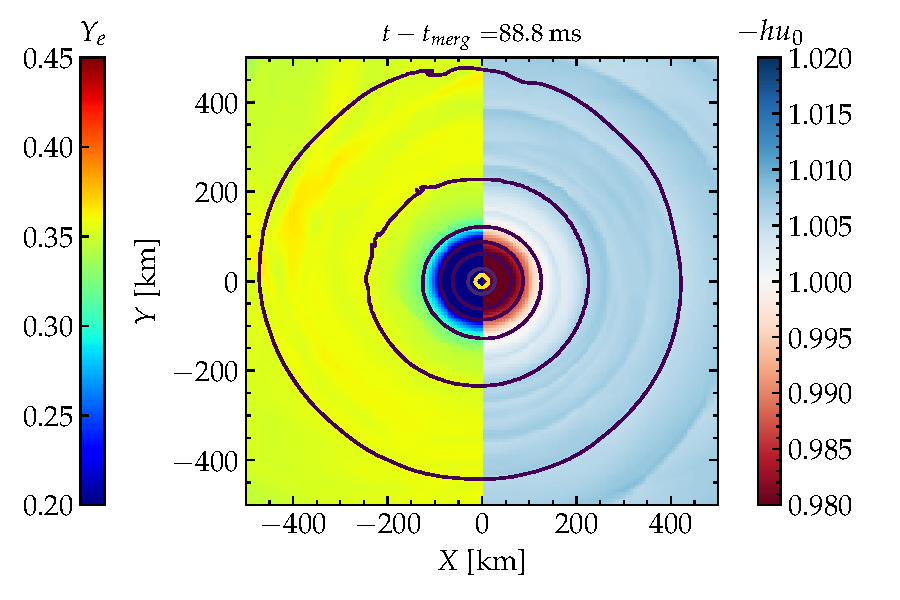
\includegraphics[width=0.49\textwidth]{slices/slice_xy_ye_hu_1.pdf}
    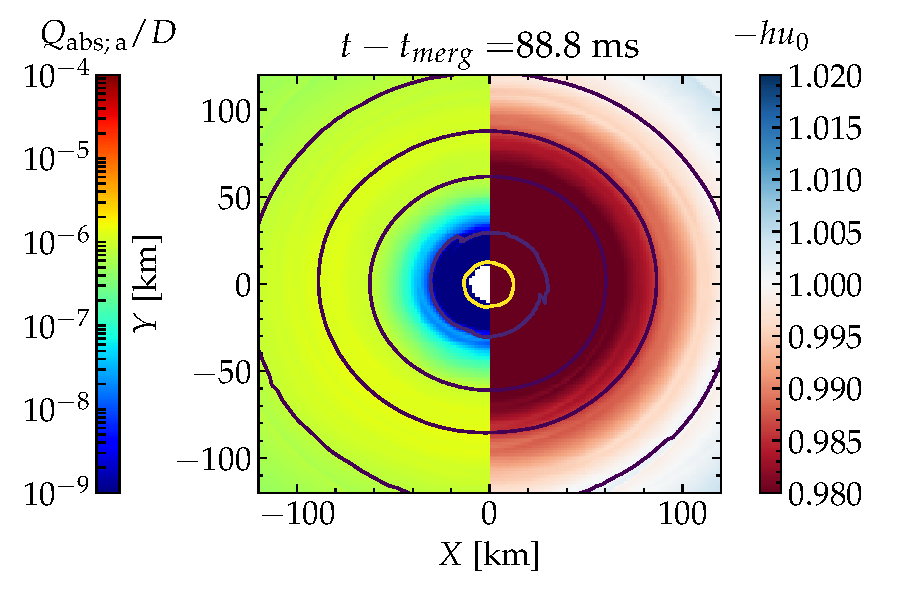
\includegraphics[width=0.49\textwidth]{slices/slice_xy_abs_energy_hu_3.pdf}
    \caption{Snapshot of the $(x,z)$ and $(x,y)$ slices of the BLh $q=1$ model at 
        ${\sim}89\,$ms after merger. Left panels: electron fraction and
        $-hu_0$. High $Y_e$ values indicate neutrino
        postprocessing and irradiation. The $-hu_0>1$ indicates the
        material that gains enough energy to become unbound at
        infinity. 
        %
        Right: $-hu_0$ and the absorption energy rate $Q_{\text{abs};\:\bar{\nu}_e}$ 
        of electron antineutrinos normalized to the fluid density $D$.
    }
    %
    \label{fig:slice:heating_hu}
\end{figure*}

In this section we investigate in detail the 
high electron fraction, polar component of the \acp{SWW}.
We propose that this outflow is mostly driven by the neutrino 
reabsorption, rather than by the dynamical mechanism responsible for the bulk of the 
\ac{SWW}.

The presence of the baryonic winds developing on the timescale of $\mathcal{O}(10)$~ms
and driven by the neutrino absorption above the remnant, where the neutrino flux is strong 
was reported before \citep[\eg][]{Perego:2014fma}. 

In this section we focus of the feducial model BLh $q=1.00$ (SR). 

In the left column of plots in Fig.~\ref{fig:slice:heating_hu} we compare 
the the Bernoulli parameter, 
$-hu_t$ (see Sec.\ref{sec:method:Bernoulli}), and the fluid electron 
fraction. 

In the right column of plots in Fig.~\ref{fig:slice:heating_hu} we compare 
the the Bernoulli parameter with the heating energy rate due to electron anti-neutrino absorption 
$Q_{\text{abs};\:\bar{\nu}_e}$ (see Sec.~\ref{method:M0:eq_for_Q}) divided by with 
$D=W\rho\sqrt{\gamma}$ (fluid's conserved rest-mass density)
We observe that the electron fraction in the polar region with angle 
from binary plane $\theta>60^{\circ}$ reaches $Y_e\sim0.35$ due to the absorption of 
electron-type neutrinos.
The strongest neutrino heating occurs in the vicinity of the remnant at densities 
$\rho\sim10^{11}$~\gcm, that roughly correspond to the region where neutrinos decouple,
the so-called neutrinosphere \citep{Endrizzi:2019trv}.

In Fig.~\ref{fig:slice:heating_hu} we compare the Bernoulli parameter, 
$-hu_t$ (see Sec.\ref{sec:method:Bernoulli}), that is always plotted 
on the right half of a panel, with the electron fraction (left 
column of plots and heating energy rate due to electron anti-neutrino absorption 
$Q_{\text{abs};\:\bar{\nu}_e}$ divided by with $D=W\rho\sqrt{\gamma}$ 
(fluid's conserved rest-mass density).
The observed correlation between the $E_\nu/D$ \red{???} and $-h u_t$ further suggests, 
that the outflow around the polar axis is driven by the neutrino absorption. 
Additionally, we found that if the neutrino absorption is not included into the 
simulation, \eg, using leakage only, the \nwind{} is absent. 
%% --- 
The collimated polar outflow can be further boosted and stabilized by the presence of the 
strong magnetic fields \citep{Bucciantini:2011kx,Ciolfi:2020hgg,Mosta:2020hlh}.
%% ---
Notably, there is not clear distinction between the \nwind{} and \ac{SWW}, especially 
at the intermediate latitudes ($\theta \sim 45^{\circ}$), where both mechanisms types of 
ejecta are present, and both, neutrino absorption and dyanmical effects driving the \ac{SWW} 
are contributing. 
%% --- 
In order to compute the mass flux of the \nwind{} an additional criterion is required. 
We consider two physically motivated criteria, the geometrical, flaggin the part of the \ac{SWW} 
and \nwind{} if it is polar, \ie, $\theta>60^{\circ}$, and the composition criterion, $Y_e > 0.35$.
%% --- 
We find that the \nwind{} is not a steady state outflow, contrary to the bulk of the \ac{SWW}.
After the initial strong rise, the mass flux rapidly decays in time, and for most models stops 
by the end of the simulations. This behaviour is independent of the criterion we use. 
We attribute it to the rise of the baryon loading above the remnant as the material gets lifted 
by thermal pressure from the disk.
The total mass of the \nwind{} is ${\sim}10^{-3}-10^{-4}M_{\odot}$. Its properties resemble those 
reported in e.g. \citet{Dessart:2008zd,Perego:2014fma,Fujibayashi:2020dvr}
Notably, in some of the works, the \nwind{} was found to require longer timescales to develop, 
achieving the quasi-steady state. 
This can be attributed to the strict criteria to isolate the \nwind{} and by the absence of the 
\ac{SWW} in other works. 
Additionally, our simulations might not be sufficiently long to achieve the donditions 
sufficient for the development of the quasi-steady state \nwind{}.
%% Additionally, as our models are at most $\sim100$~ms long, the conditions required for the steady 
%% state \nwind{} might not been achieved.



%% =======================================================
%%
%%                   Disc structure
%%
%% =======================================================


\section{Remnant disk structure}

\begin{figure}[t]
    \centering
    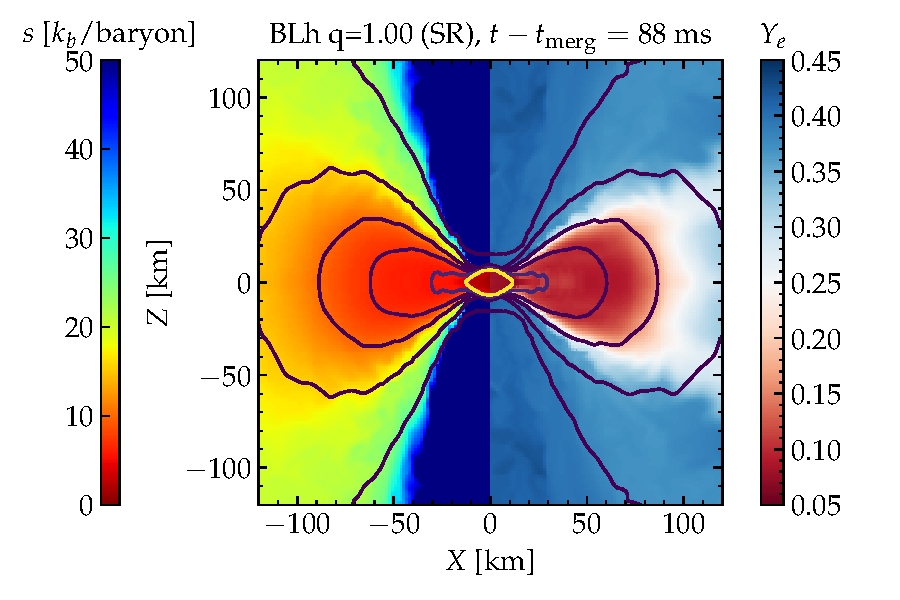
\includegraphics[width=0.49\textwidth]{disk/final_structure/slice_xz_entr_ye_blh_q1_rl3.pdf}
    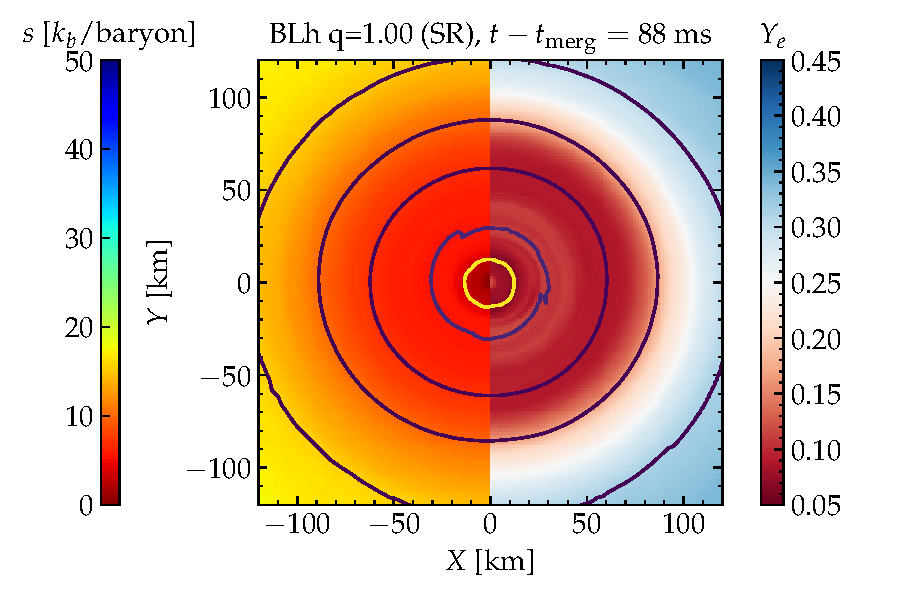
\includegraphics[width=0.49\textwidth]{disk/final_structure/slice_xy_entr_ye_blh_q1_rl3.pdf}
    \caption{Entropy and electron fraction on the $(x,z)$ (top) and
        $(x,y)$ planes (bottom) for the remnant of BL $q=1$ at the end
        of the simulation. Each plot is divided vertically, with entropy
        being color-coded on the left and electron fraction on the
        right. Solid contours stand for rest muss density. Counting from
        the center, the values are $[10^{13}, 10^{12}, 10^{11}, 10^{10},
        10^{9}]$ g cm$^{-3}$, with the inner most contour encompassing
        the remnant.
        (Adapted from \citet{Nedora:2020pak})
    }  
    \label{fig:snapshots_xy_ye_entr}
\end{figure}

\begin{figure*}[t]
    \centering 
    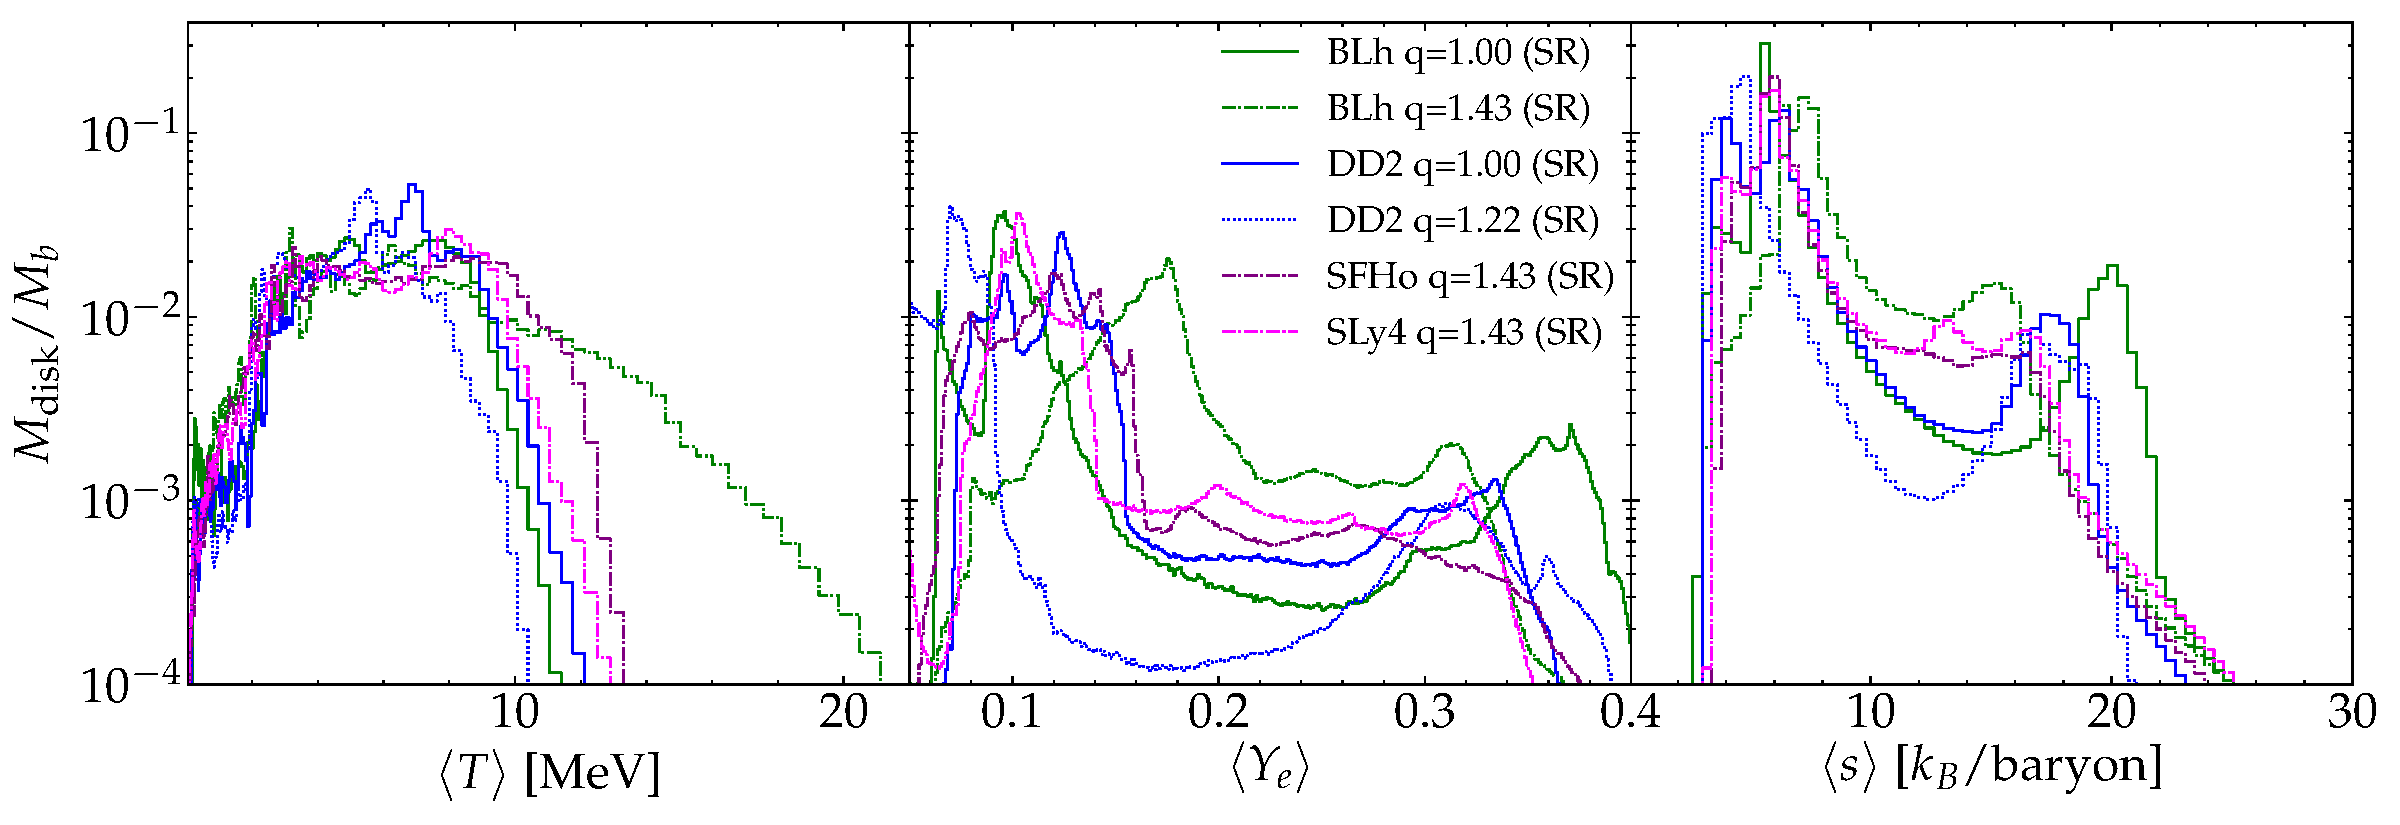
\includegraphics[width=0.95\textwidth]{disk/final_structure/disk_hist_shared.pdf}
    \caption{Composition of the disks at the end of the long-lived
        remnants simulations. The histograms refer to the temperature $T$
        (left),
        electron fraction $Y_e$
        (middle) and entropy $s$ (right).
        (Adapted from \citet{Nedora:2020pak})
    }
    \label{fig:final_disk_struct_hist_long}
\end{figure*}

In this section we discuss the final structure and properties of the disk, 
focusing on the models with long-lived \ac{MNS} remnants.
The properties are extracted at typical time $\sim60{-}100$~ms after merger.

We find that the generally the disk is optically thick.
The disk' RMS openning appears to be independent of the \ac{EOS} and \mr{} and
is $\langle\theta\rangle_{\text{rms}}\sim60^{\circ}$. 
The radial extend of the disk, however increases with the \ac{EOS} softness and 
binary \mr{}.
Similarly, the final disk mass is larger for the unequal mass binaries, 
ranging overall between ${\sim}0.1M_{\odot}$ and ${\sim}0.4M_{\odot}$
(see Tab.~\ref{tab:sim})..
Notably, for models with long-lived remnants the disk mass is larger,
that for the those with long-lived remnants. This can be attributed to the 
rapid accretion onto a \ac{BH} that removes $\sim50\%$ of the disk mass.
%% ---
We investigate the overall statistical properties of the disk mass for all our models
and those available in the literature in Sec.\ref{sec:results:Statistics:Mdisk}
\gray{
    The mean value of the disk mass in out models is 
    $\overline{M}_{\text{disk}}=(0.161 \pm 0.083)M_{\odot}$,
    where the standard deviation is also reported.
    %% ---
    Similarly to the dynamical ejecta we fit the disk masses with the 
    second order polynomial in $(q,\tilde{\Lambda})$.
    The coefficients of Eq.~\eqref{eq:fit:poly22}
    for this fit are given in Tab.~\ref{tab:fitpoly22coefs}.
    A more detailed study with various fitting formulas and extended
    datasets from the literature is reported in a companion paper.
}

Next, we consider the composition of the disk at the end of the simulation.
%% --- 
The mass-averaged temperature, electron fraction and entropy per baryon
are for several models are shown in Fig.~\ref{fig:final_disk_struct_hist_long}.
%% ---
We observe that the mass-weighted distribution of the entropy and electron 
fraction show a bimodal structure, which is more pronounced for the 
equal mass binaries. 
Regarding entropy, two peaks are present in the distribution:
a peak low entropy $s\sim5-10k_B/$baryon, that depends weakly of the 
\ac{EOS} and \mr{} and corresponds to the bulk, mildly shocked, material. 
The second peak is found at higher entropy, $s\sim15-22k_B/$baryon.
It corresponds fo the strongly shocked material and is more prominent 
in models with softer \ac{EOS}.
Notably, in the models with higher \mr{}, the second peak is located 
at lower $s$.
The mass-weighted distribution of the electron fraction 
displays a similar double-peak structure.
The low $Y_e$ peak that corresponds to the neutrino-shielded part of the 
disk is located around the $Y_e\sim0.1$.
The high $Y_e$ peak is located at $Y_e\sim0.3-0.4$ and corresponds to the outer parts of the disk, subjected to a strong neutrino irradiation.

In Fig.~\ref{fig:snapshots_xy_ye_entr} we show the electron fraction 
and entropy per baryon on the $xy$ and $xz$ slices of the equal 
mass model with BLh \ac{EOS}.
The plot shows, that the two peaks in the mass-weighted distribution 
of electron fraction and entropy correspond to different regions within the disk.

Overall, the most of the disk matter has temperature of $T\sim 1-10\,$MeV, with the innermost parts being hotter then the outer outermost. 
However, the disk temperature distribution appears to be largely independent of the \ac{EOS} and \mr{}

\red{Paragraph on the secular ejecta has been moved to 
    GW170817 application}

%% =======================================================
%%
%%                   Conclusion
%%
%% =======================================================




%% ========================================================================================

\section{Statistics of the \ac{DE} parameters and disk mass}

\red{CONTENT OF THE FIT PAPER}


\section{Application to \GW{}}


\begin{figure*}[t]
    \centering 
    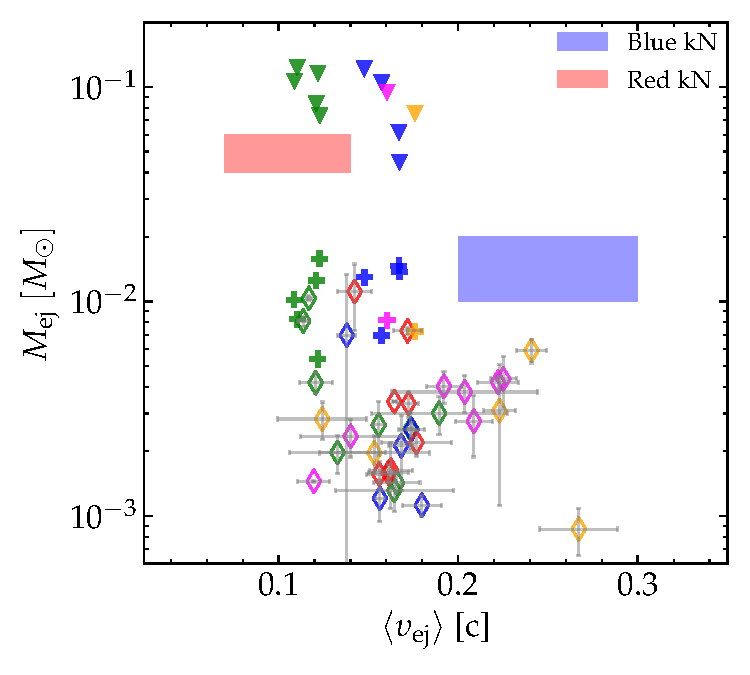
\includegraphics[width=0.48\textwidth]{ejecta_dyn/summary/ej_mej_vej_our2.pdf}
    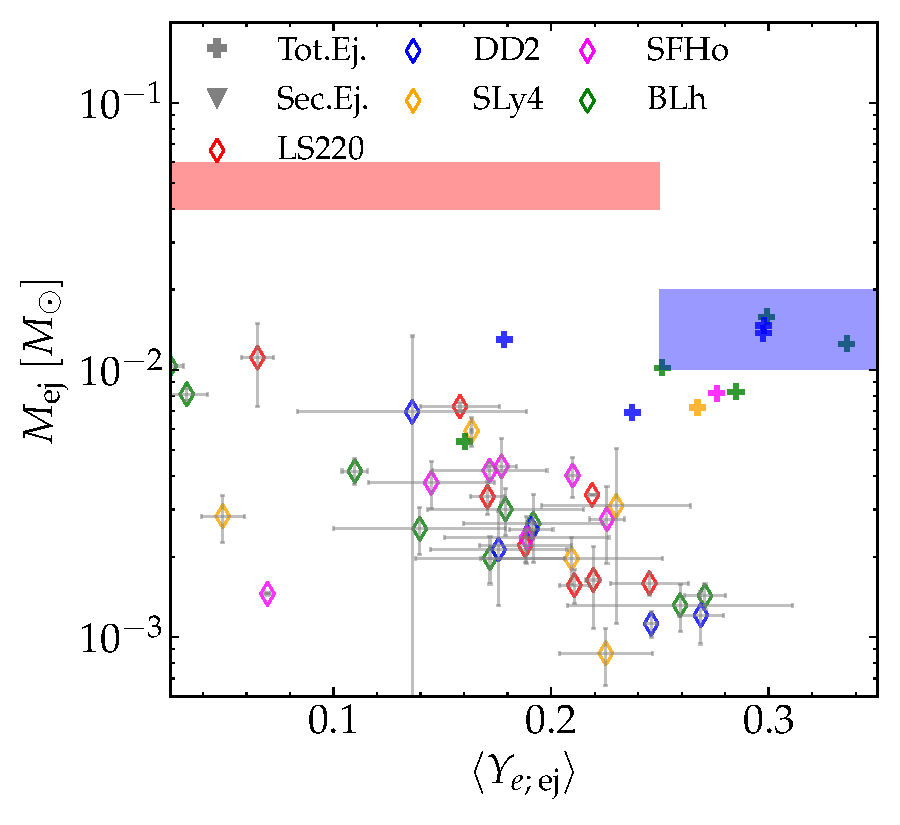
\includegraphics[width=0.48\textwidth]{ejecta_dyn/summary/ej_mej_yeej_our2.pdf}
    \caption{
        Summary of the ejecta properties of our models.
        %
        Diamonds mark the dynamical ejecta, crosses include the
        contribution of the \swind{} for the long-lived models, 
        triangles are an estimate of the total ejecta mass on a secular
        timescale, assuming $40\%$ of the disk mass is unbounded on
        secular timescales.         
        The ejecta mass is shown is terms of the mass-averaged velocity
        (left) and of the averaged electron fraction (right).
        %
        The filled blue and red patches are the expected values of
        ejecta mass and velocity for blue and red components of
        AT2017gfo compiled by \cite{Siegel:2019mlp}, based on
        \cite{Villar:2017wcc}. 
        Adopted from \citet{Nedora:2020pak}.
    }
    %
    \label{fig:ejecta:dyn:ds_sww}
\end{figure*}


%% from main paper, referencing the fitpaper Poly22 fits and SWW + DE
\red{THis can be augmented with Radio afterglow}

%% === FROM DYNAMICAL EJECTA SECTION of MAIN PAPER
Here we discuss the application of our results to \GW{}.


\subsection{Dynamical Ejecta}


%% ---
First, we asses the ejecta parameters that our fitting models, 
obtained in section \ref{sec:ejecta_disk_statisitcs} would provide for the \GW{}.
%% --- 
Considering the $90\%$ credible intervals estimated for $q$ and $\tilde{\Lambda}$ 
from LIGO-Virgo GW analysis
\citep{TheLIGOScientific:2017qsa,Abbott:2018wiz,De:2018uhw,Abbott:2018exr},
i.e.~$\tilde{\Lambda}=300_{-190}^{+500}$ and $q\in[1., 1.37]$. 
and using the errorbars formulas developed in \cite{Radice:2018pdn}, we find that
$\amd \in [0.72, 7.52] \times 10^{-3}\: M_{\odot}$
and
$\avd \in [0.16, 0.39]$c 
and 
$\ayd \in [0.11, 0.23]$.
Notably, these values do not agree with those inferred for \AT{} by the spherical, 
two-component kilonova models \citep{Villar:2017wcc}.
Analysis of a compiled set of kilonova fitting models provides a broad range of ejecta 
parameters \citep{Siegel:2019mlp}:
$M_{\text{ej}}^{\text{red}}\in(4, 6)\times10^{-2}M_{\odot}$ and
$\upsilon_{\text{ej}}^{\text{red}}\in(0.07, 0.14)$ for the red component, while
$M_{\text{ej}}^{\text{blue}}\in[1, 2]\times10^{-2}M_{\odot}$ and 
$\upsilon_{\text{ej}}^{\text{blue}}\in[0.2, 0.3]$ for the blue component.
%% ---
With respect to our results for \ac{DE}, however, 
none of the kilonova components can be well explained.
%% ---
In Fig.~\ref{fig:ejecta:dyn:ds_sww} we show the ejecta properties from
all our models (diamonds) and the parameters inferred from the
observations as red and blue boxes. 
%% --- 
With respect to the red component, we observe that \ac{DE} from our models 
have too high average velocities and not nearly enough mass.
This result suggests that an additional, low $Y_e$ ejecta component is required
in order to explain the \AT{} red component 
\citep{Perego:2017wtu,Kawaguchi:2018ptg,Nedora:2019jhl}.
%% --- 
A more thorough analysis of the \AT{} with better ejecta models and advanced
radiation transport kilonova simulations are not part of the present work 
and will be addressed in the future.


\subsection{Spiral-wave wind}


The \ac{SWW} could be a significant contributor to the \AT{}, assuming the remnant of 
\GW{} \ac{MNS} merger survived for $\mathcal{O}(100)$~ms.
%% ---- 
In Fig.~\ref{fig:ejecta:dyn:ds_sww} we report the total
(dynamical+\swind{}) ejecta mass and mass-averaged velocity for the
simulated long-lived BNS (crosses).
%% ---
Notably, the total ejecta mass of three of our models, 
BLh $q=1.18$, BLh $q=1.42$ and  DD2 is $q=1$ are in agreemnt with the epected values 
for the blue compoent of the \AT{} 
(obtained using the two-component fit \citep{Villar:2017wcc})

\red{
    [ LETTER STUFF COULD GO HERE ]
    a multi-component fitting model that explicitly accounts
    for the \swind{} can fit the early blue
    emission from AT2017gfo \citep{Nedora:2019jhl}
}

The high electron fraction of the \ac{SWW} however would result in a lanthanides-poor
composition of the outflow. Thus, the \ac{SWW} cannot explain the observed emission 
for the high opacity, lanthanides-rich material.
%% ---
Simulations with advanced physics of a \ac{MNS} mergers on a timescales $>100$~ms are 
required to asses the contribution from other outflow mechanisms, \red{that we will discuss below} 
\citep{Lee:2009uc,Fernandez:2015use,Siegel:2017nub,Fujibayashi:2017puw,Fernandez:2018kax,Radice:2018xqa}.


\subsection{Secular Ejecta}


On the timescale of seconds, much longer than the evolution of 
presented here simulations, the nuclear recombination can unbind 
a fraction of the disk mass. 
Analytical estimates and simulations with various approximations show that up tp ${\sim}40\%$ of the disk can be ejected via viscous processes with an typical velocity ${\lesssim}0.1\,$c
\citep{Lee:2009uc,Fernandez:2015use,Wu:2016pnw,Siegel:2017nub,Fujibayashi:2017puw,Fernandez:2018kax,Radice:2018xqa,Fujibayashi:2020dvr}.

Adapting the fix fraction of the $40\%$ of the disk mass, we estimate 
that about  ${\sim}0.05\, M_{\odot}$ would be ejected in a form of 
secular winds. We include this estimate for every simulation
with the long-lived \ac{MNS} remnant in Fig.~\ref{fig:ejecta:dyn:ds_sww} (lower triangles).
The estimated mass is sufficient to explain
the red component of AT2017gfo, as inferred from the two-components kN
models of \cite{Villar:2017wcc}. 







%% ---------------------
Sources with time delay are preferred by studies of very metal poor stars that indluded the time delay for r-process elements
to diffuse through ISM, \citep{Tarumi:2021xvw}. 
A winds from proto-nuetron are also contributors to the $r$-process budget \cite{Vincenzo:2021rvw}

\red{The remnant is losing anular momentum while disk gains on shortly after merger is due to gravitational torque \cite{Shibata:2019wef}}
